\documentclass[12pt]{report}
\usepackage{graphicx}     %Note graphics<graphicx<epsfig
\usepackage[table,xcdraw, dvipsnames]{xcolor}
\usepackage{hyperref} %written by Sebastian Rahtz
%\usepackage{subeqn}    %allows equations 1a, 1b
%\usepackage{subfig}    %allows figures 1a, 1b
\usepackage{amsmath}
\usepackage{amssymb}
\usepackage{xurl}
\usepackage{bbm}%for indicator function
%\bibliographystyle{alpha}
\usepackage{floatrow}
\usepackage[normalem]{ulem}
\usepackage{tikz}
\usepackage{xparse, expl3, istgame, makecell}



\usepackage{tocloft}

%\usepackage{emoji}

% Adjust number widths
\setlength{\cftchapnumwidth}{2em}
\setlength{\cftsecnumwidth}{3.2em}
\setlength{\cftsubsecnumwidth}{3.5em}

\usepackage[toc,page]{appendix}
\usepackage[nottoc]{tocbibind}

\usepackage[color,matrix,frame,arrow,curve]{xy}
\usepackage[shortlabels]{enumitem}
\usepackage{array}
\usepackage{pdflscape}
\usepackage{multicol, multirow}
\usepackage{ctable}
\usepackage{dirtree}
\usepackage{subfig}
\usepackage{longtable}
\usepackage{pdfpages}
\usepackage{esvect}

\usepackage{bm}

%\usepackage{fdsymbol}
%\usepackage{animate}% play animation

\usepackage[vlined,ruled]{algorithm2e}
\newcommand{\mycommfont}[1]{\small\ttfamily\textcolor{blue}{#1}}
\SetCommentSty{mycommfont}

%highlighting
\usepackage{mdframed}

\usepackage[makeroom]{cancel}

\usepackage{pdfpages}
\usepackage{hyperxmp}
\usepackage{tensor}

% this escapes the underscore in text
%\usepackage[T1]{fontenc}
%\usepackage{underscore}

\paperheight=11in
\topmargin=0in
\headheight=0in
\headsep=0in
\topskip=0in
\textheight=8.5in
\footskip=.5in


\paperwidth=8.5in
\oddsidemargin=.25in
\evensidemargin=.25in
\textwidth=6.0in
\parindent=.5in

\newcommand{\bcen}[0]{\begin{array}{c}}
\newcommand{\ecen}[0]{\end{array}}
\newcommand{\twoarrows}[0]{\uparrow\downarrow}
\newcommand{\circone}{\tiny (1)}


\newcommand{\chapquote}[3]{\begin{quotation} \textit{#1} \end{quotation} \begin{flushright} - #2, \textit{#3}\end{flushright} }

\newtheorem{claim}{Claim}
\newcommand{\proof}[0]{{\bf proof:} }
\newcommand{\qed}[0]{\quad\newline \noindent{\bf QED }}

\newcommand{\upto}[0]{-}
\newcommand{\XT}[2]{{\substack{#1\\#2}}}

\newcommand{\bra}[1]{\langle#1|}
\newcommand{\ket}[1]{|#1\rangle}
\newcommand{\av}[1]{\left\langle#1\right\rangle}
\newcommand{\pder}[2]{\frac{\partial#1}{\partial#2}}
\newcommand{\der}[2]{\frac{d#1}{d#2}}
\newcommand{\tr}[0]{{\rm tr }}
\newcommand{\beq}{\begin{equation}}
\newcommand{\eeq}{\end{equation}}
\newcommand{\bsub}{\begin{subequations}}
	\newcommand{\esub}{\end{subequations}}
\newcommand{\beqa}{\begin{eqnarray}}
\newcommand{\eeqa}{\end{eqnarray}}
\newcommand{\rarrow}[0]{\rightarrow}
\newcommand{\larrow}[0]{\leftarrow}
\newcommand{\uarrow}[0]{\uparrow}
\newcommand{\darrow}[0]{\downarrow}
\newcommand{\Rarrow}[0]{\Rightarrow}
\newcommand{\nRarrow}[0]{\nRightarrow}
\newcommand{\Larrow}[0]{\Leftarrow}
\newcommand{\nLarrow}[0]{\nLeftarrow}
\newcommand{\ul}[1]{\uline{#1}}
\newcommand{\ol}[1]{\overline{#1}}
\newcommand{\CC}[0]{{ \mathbb{C}} }
\newcommand{\EE}[0]{{ \mathbb{E}} }
\newcommand{\FF}[0]{{ \mathbb{F}} }
\newcommand{\GG}[0]{{ \mathbb{G}} }
\newcommand{\NNN}[0]{ {\mathbb{N}}} %\NN already defined
\newcommand{\PP}[0]{{ \mathbb{P}} }
\newcommand{\RR}[0]{{ \mathbb{R}} }
\newcommand{\TT}[0]{{ \mathbb{T}} }
\newcommand{\WW}[0]{ {\mathbb{W}}}
\newcommand{\XX}[0]{{ \mathbb{X}} }
\newcommand{\YY}[0]{{ \mathbb{Y}} }
\newcommand{\ZZ}[0]{ {\mathbb{Z}}}

\renewcommand{\Re}{{\rm Re}}
\renewcommand{\Im}{{\rm Im}}



\newcommand{\ground}{{}_{\stackrel{\stackrel{\displaystyle{\bot}}{-}}{.}}}
\newcommand{\norm}[1]{\parallel#1\parallel}
\newcommand{\eqdef}[0]{\;\;\stackrel{\text{def}}{=}\;\;}

\newcommand{\heavy}[0]{\mathbf{H}}

\newcommand{\rva}[0]{{\ul{a}}}
\newcommand{\rvb}[0]{{\ul{b}}}
\newcommand{\rvc}[0]{{\ul{c}}}
\newcommand{\rvd}[0]{{\ul{d}}}
\newcommand{\rve}[0]{{\ul{e}}}
\newcommand{\rvf}[0]{{\ul{f}}}
\newcommand{\rvg}[0]{{\ul{g}}}
\newcommand{\rvh}[0]{{\ul{h}}}
\newcommand{\rvi}[0]{{\ul{i}}}
\newcommand{\rvj}[0]{{\ul{j}}}
\newcommand{\rvk}[0]{{\ul{k}}}
\newcommand{\rvl}[0]{{\ul{l}}}
\newcommand{\rvll}[0]{{\ul{\ell}}}
\newcommand{\rvm}[0]{{\ul{m}}}
\newcommand{\rvn}[0]{{\ul{n}}}
\newcommand{\rvo}[0]{{\ul{o}}}
\newcommand{\rvp}[0]{{\ul{p}}}
\newcommand{\rvq}[0]{{\ul{q}}}
\newcommand{\rvr}[0]{{\ul{r}}}
\newcommand{\rvs}[0]{{\ul{s}}}
\newcommand{\rvt}[0]{{\ul{t}}}
\newcommand{\rvu}[0]{{\ul{u}}}
\newcommand{\rvv}[0]{{\ul{v}}}
\newcommand{\rvw}[0]{{\ul{w}}}
\newcommand{\rvx}[0]{{\ul{x}}}
\newcommand{\rvy}[0]{{\ul{y}}}
\newcommand{\rvz}[0]{{\ul{z}}}


\newcommand{\rvA}[0]{{\ul{A}}}
\newcommand{\rvB}[0]{{\ul{B}}}
\newcommand{\rvC}[0]{{\ul{C}}}
\newcommand{\rvD}[0]{{\ul{D}}}
\newcommand{\rvE}[0]{{\ul{E}}}
\newcommand{\rvF}[0]{{\ul{F}}}
\newcommand{\rvG}[0]{{\ul{G}}}
\newcommand{\rvH}[0]{{\ul{H}}}
\newcommand{\rvI}[0]{{\ul{I}}}
\newcommand{\rvJ}[0]{{\ul{J}}}
\newcommand{\rvK}[0]{{\ul{K}}}
\newcommand{\rvL}[0]{{\ul{L}}}
\newcommand{\rvM}[0]{{\ul{M}}}
\newcommand{\rvN}[0]{{\ul{N}}}
\newcommand{\rvO}[0]{{\ul{O}}}
\newcommand{\rvP}[0]{{\ul{P}}}
\newcommand{\rvQ}[0]{{\ul{Q}}}
\newcommand{\rvR}[0]{{\ul{R}}}
\newcommand{\rvS}[0]{{\ul{S}}}
\newcommand{\rvT}[0]{{\ul{T}}}
\newcommand{\rvU}[0]{{\ul{U}}}
\newcommand{\rvV}[0]{{\ul{V}}}
\newcommand{\rvW}[0]{{\ul{W}}}
\newcommand{\rvX}[0]{{\ul{X}}}
\newcommand{\rvY}[0]{{\ul{Y}}}
\newcommand{\rvZ}[0]{{\ul{Z}}}

\newcommand{\rvbeta}[0]{{\ul{\beta}}}
\newcommand{\rvxi}[0]{{\ul{\xi}}}
\newcommand{\rvzeta}[0]{{\ul{\zeta}}}
\newcommand{\rvtheta}[0]{{\ul{\theta}}}
\newcommand{\rvmu}[0]{{\ul{\mu}}}
\newcommand{\rvsig}[0]{{\ul{\sigma}}}
\newcommand{\rvDel}[0]{{\ul{\Delta}}}
\newcommand{\rvtau}[0]{{\ul{\tau}}}

\newcommand{\cala}[0]{{\cal A}}
\newcommand{\calb}[0]{{\cal B}}
\newcommand{\calc}[0]{{\cal C}}
\newcommand{\cald}[0]{{\cal D}}
\newcommand{\cale}[0]{{\cal E}}
\newcommand{\calf}[0]{{\cal F}}
\newcommand{\calg}[0]{{\cal G}}
\newcommand{\calh}[0]{{\cal H}}
\newcommand{\cali}[0]{{\cal I}}
\newcommand{\calk}[0]{{\cal K}}
\newcommand{\call}[0]{{\cal L}}
\newcommand{\calm}[0]{{\cal M}}
\newcommand{\caln}[0]{{\cal N}}
\newcommand{\calo}[0]{{\cal O}}
\newcommand{\calp}[0]{{\cal P}}
\newcommand{\calq}[0]{{\cal Q}}
\newcommand{\calr}[0]{{\cal R}}
\newcommand{\cals}[0]{{\cal S}}
\newcommand{\calt}[0]{{\cal T}}
\newcommand{\calu}[0]{{\cal U}}
\newcommand{\calv}[0]{{\cal V}}
\newcommand{\calw}[0]{{\cal W}}
\newcommand{\calx}[0]{{\cal X}}
\newcommand{\caly}[0]{{\cal Y}}
\newcommand{\calz}[0]{{\cal Z}}

%\newcommand{\diamante}[1]{\Big\langle#1\Big\rangle}
\newcommand{\diamante}[1]{*++[F=]{#1}}
%\newcommand{\corchete}[1]{\Big\{#1\Big\}}
\newcommand{\corchete}[1]{#1}
\newcommand{\cuadro}[1]{*++[F]{#1}}

\newcommand{\Pmat}[4]{\calp\left[
\begin{array}{cc}#1&#2\\#3&#4
\end{array}\right]}

%\newcommand{\PN}[0]{PN^{0,0}_{1,1}}
%\newcommand{\PS}[0]{PS^{1,1}_{0,0}}
\newcommand{\PN}[0]{PN}
\newcommand{\PS}[0]{PS}

\newcommand{\lam}[0]{\lambda}
\newcommand{\Lam}[0]{\Lambda}
\newcommand{\alp}[0]{\alpha}
\newcommand{\eps}[0]{\epsilon}
\newcommand{\s}[0]{\sigma}
\newcommand{\su}[0]{{\Sigma}}

\newcommand{\pp}[0]{\mathbb{P}}
\newcommand{\dbm}[0]{{
		[1,\partial_{b},\partial_{m}]
}}

\newcommand{\dg}[0]{{[1, \partial_{\theta_G}]}}
\newcommand{\dd}[0]{{[1, \partial_{\theta_D}]}}
\newcommand{\dgd}[0]{{[1, \partial_{\theta_G}, \partial_{\theta_D}]}}

\newcommand{\veca}[0]{{\vec{a}}}
\newcommand{\vecb}[0]{{\vec{b}}}
\newcommand{\vecc}[0]{{\vec{c}}}
\newcommand{\vecd}[0]{{\vec{d}}}
\newcommand{\vecf}[0]{{\vec{f}}}
\newcommand{\vech}[0]{{\vec{h}}}
\newcommand{\vecr}[0]{{\vec{r}}}
\newcommand{\vecs}[0]{{\vec{s}}}
\newcommand{\vecu}[0]{{\vec{u}}}
\newcommand{\vecx}[0]{{\vec{x}}}
\newcommand{\vecy}[0]{{\vec{y}}}
\newcommand{\vechy}[0]{{\vec{\haty}}}
\newcommand{\vtheta}[0]{{\vec{\theta}}}

\newcommand{\haty}[0]{{\widehat{y}}}
\newcommand{\hatx}[0]{{\widehat{x}}}
\newcommand{\hata}[0]{{\widehat{a}}}
\newcommand{\hatr}[0]{{\widehat{r}}}


\newcommand{\cond}[0]{{\:\mathbf{|}\:}}
\newcommand{\mymathbf}[1]{#1}

\newcommand{\ranvec}[1]{\ul{\vec{#1}}}
\newcommand{\indi}[0]{\mathbbm{1}}
\newcommand{\smoid}[0]{{\rm smoid}}
\newcommand{\lodds}[0]{{\rm lodds}}
\newcommand{\expit}[0]{{\rm expit}}
\newcommand{\logit}[0]{{\rm logit}}
\newcommand{\sign}[0]{{\rm sign}}

\renewcommand{\labelitemii}{$\bullet$}

\newcommand{\HAT}[1]{{\widehat{#1}}}
\newcommand{\TIL}[1]{{\widetilde{#1}}}
\newcommand{\tild}[0]{{\TIL{d}}}
\newcommand{\tile}[0]{{\TIL{e}}}
\newcommand{\tilg}[0]{{\TIL{g}}}
\newcommand{\tilu}[0]{{\TIL{u}}}
\newcommand{\tilx}[0]{{\TIL{x}}}
\newcommand{\tilP}[0]{{\TIL{P}}}
\newcommand{\tilPT}[0]{{\TIL{P}_\theta}}

\newcommand{\maparrow}[1]
{\xymatrix{\ar[r]_{#1}&}}


\newcommand{\ucalm}[0]{\ul{\calm}}

\newcommand{\bool}[0]{\{0,1\}}

\newcommand{\argmin}{\mathop{\mathrm{argmin}}\limits}
\newcommand{\argmax}{\mathop{\mathrm{argmax}}\limits}

\newcommand{\softmax}[0]{{\rm softmax}}

\newcommand{\A}[0]{\wedge}
\newcommand{\V}[0]{\vee}
\newcommand{\xor}{\oplus}
\newcommand{\bigA}[0]{\bigwedge}
\newcommand{\bigV}[0]{\bigvee}
\newcommand{\bigxor}{\bigoplus}


\newcommand{\rdart}[0]{\Rightarrow}
\newcommand{\ldart}[0]{\Leftarrow}
\newcommand{\rveps}[0]{\ul{\eps}}

\newcommand{\hatvar}[0]{\widehat{\sigma^2}}
\newcommand{\ptp}[0]{{(t)}}

\newcommand{\tseries}[1]{{\{#1\}_{\forall t}}}

\newcommand{\xbeta}[0]{X_\s^T\beta}
\newcommand{\xtau}[0]{X_\s^T\tau}

\newcommand{\LeafAr}[1]{
\ar@{->}@/_1pc/[#1]
\ar@{<-}@/^1pc/[#1]
}
\newcommand{\Rect}[1]{*++[F-]{#1}}
\newcommand{\Circle}[1]{*++[o][F-]{#1}}
\newcommand{\DCircle}[1]{*++[o][F=]{#1}}
\newcommand{\PinkCircle}[1]{*++[o][F-][F**:pink]{#1}}
\newcommand{\PinkDCircle}[1]{*++[o][F=][F**:pink]{#1}}

\newcommand{\OTO}[0]{\boxed{\bf \checkmark OTO}\;}
\newcommand{\COTO}[0]{\boxed{\bf \checkmark OTO}\;}

%\xymatrix{
%&a
%\\
%\DCircle{\rvx}\LeafAr{ru}&
%}

%https://tex.stackexchange.com/questions/208905/loops-of-different-sizes

\newcommand{\loopup}[2]{ % \ar@(ul,ur) size is like 3
\ar@`{[]+/ul+#1pc/,[]+/ur+#1pc/}#2[]}
\newcommand{\loopdown}[2]{ % \ar@(ul,ur) size is like 3
\ar@`{[]+/dl+#1pc/,[]+/dr+#1pc/}#2[]}
\newcommand{\loopright}[2]{ % \ar@(ul,ur) size is like 3
\ar@`{[]+/dr+#1pc/,[]+/ur+#1pc/}#2[]}
\newcommand{\loopleft}[2]{ % \ar@(ul,ur) size is like 3
\ar@`{[]+/dl+#1pc/,[]+/ul+#1pc/}#2[]}

% test code
%\xymatrix{
%\rva\loopup{3}{@[green]_r}
%&
%\rvb\loopdown{3}{@[red]_r}
%&
%\rvc\loopright{3}{@[blue]_r}
%\\
%\rvd\loopleft{3}{@[violet]_r}
%}


\newcommand{\redminus}[0]{{\color{red}\bm{\;-\;}}} 
\newcommand{\redplus}[0]{{\color{red}\bm +}}
\newcommand{\redzero}[0]{{\color{red}\bm 0}}
\newcommand{\redominus}[0]{{\color{red}\bm\ominus}} 
\newcommand{\redoplus}[0]{{\color{red}\bm\oplus}}

\newcommand{\pospart}[1]{\left(#1\right)^{\geq 0}}

\newcommand{\posvec}[1]{
\left(#1\right)^{\text{+vec}}
}

\newcommand{\petriar}[3]{{\ar@{.>}@/_1pc/[#1]|*++[o][F-]{#2}
\ar[#1]
\ar@{<.}@/^1pc/[#1]|*++[o][F-]{#3}
}}

\newcommand{\fbackar}[3]{{
\ar@{->}@/_1pc/[#1]|{\color{red}\bm\;#2\;}
\ar@{<-}@/^1pc/[#1]|{\color{red}\bm\;#3\;}
}}

%\newcommand{\timesar}[1]{
%\ar@<.8ex>@{>-<}[#1]|{\bigotimes}
%\ar@<-.2ex>@{<->}[#1]|.
%}

\newcommand{\widefbackar}[3]{{
\ar@{->}@/_2pc/[#1]|{\color{red}#2}
\ar@{<-}@/^2pc/[#1]|{\color{red}#3}
}}

% downstream red
\newcommand{\petriarDR}[3]{\ar@[red]@{->}@/_1pc/[#1]|*++[o][F-]{#2}
\ar[#1]
\ar@{<.}@/^1pc/[#1]|*++[o][F-]{#3}
}

% upstream red
\newcommand{\petriarUR}[3]{\ar@{.>}@/_1pc/[#1]|*++[o][F-]{#2}
\ar[#1]
\ar@[red]@{<-}@/^1pc/[#1]|*++[o][F-]{#3}
}

%arguments phi1, phi2, phi3, e
\newcommand{\rbd}[4]{
\xymatrix@-1.3pc{
&#1\ar[d]&&#2\ar[d]
\\
&\rvx_1\ar[rr]
&&
\rvx_2
\ar `r[rd][rd]
\\
0\ar`u[u][ru]
\ar`d[dr][rrd]
&&&&\rvA\ar[r]&#4
\\
&&
\rvx_3
\ar `r[rru][rru]
\\
&&#3\ar[u]
}
}

\newcommand{\rulezeroif}[0]{
If $(\rvb. \perp \rva.
|\rvr., \rvs.)$ \ruleieH
in $G_{amp}=G$, then}
\newcommand{\rulezerothen}[0]{
$\rva. \rightleftarrows 1$
}

\newcommand{\ruleieH}[0]{
(i.e., $H(\rvb. : \rva.
| \rvr., \rvs.)=0$) }

\newcommand{\rulezeroP}[0]{
P_{G_e}(b.|a.,r.,s.)=P_{G_{e}}(b.|r., s.)}

\newcommand{\rulezeroH}[0]{
H(\rvb.:\rva.|\rvr.,\rvs.)=0}

\newcommand{\rulezeropic}[0]{
\xymatrix@C=1pc@R=1pc{
&r.\ar[dr]
&s.\ar[d]
\\
a.\ar[rr]
&&b.
&=
}
\xymatrix@C=1pc@R=1pc{
&r.\ar[dr]&s.\ar[d]
\\
a.\ar[rr]|0
&&b.
}}

\newcommand{\ruleoneif}[0]{
If $(\rvb. \perp \rva.
|\rvr., \rvs.)$ \ruleieH
in $G_{amp}=\cald_{\rvr.} G$, then}
\newcommand{\ruleoneshort}[0]{
If $(\rvb. \perp \rva.
|\rvr., \rvs.)$, then
$\cald\rva. \rightleftarrows \rva.$
}

\newcommand{\ruleoneP}[0]{
P_{G_e}(b.|a., \cald\rvr.=r.,s.)=
P_{G_{e}}(b.|\cald\rvr.=r., s.) }

\newcommand{\ruleoneH}[0]{
H(\rvb.:\rva.|\cald\rvr.,\rvs.)=0}

\newcommand{\ruleonepic}[0]{
\xymatrix@C=1pc@R=1pc{
&\cald\rvr.=r.\ar[dr]
&s.\ar[d]
\\
a.\ar[rr]
&&b.
&=
}
\xymatrix@C=1pc@R=1pc{
&\cald\rvr.=r.\ar[dr]
&s.\ar[d]
\\
a.\ar[rr]|0
&&b.
}}

\newcommand{\ruletwoif}[0]{
If $(\rvb.\perp \rva. |
 \rvr., \rvs.)$ \ruleieH
in $G_{amp}=\call_{\rva.}\cald_{\rvr.} G$,
 then}
 
\newcommand{\ruletwoshort}[0]{
If $(\rvb.\perp \rva. |
 \rvr., \rvs.)$
in $G_{amp}=\call_{\rva.}\cald_{\rvr.} G$, then
$\cald\rva. \rightleftarrows \rva.$
}

\newcommand{\ruletwoP}[0]{
P_{G_e}(b.|\cald\rva.=a., \cald\rvr.=r., s.)=
P_{G_{e'}}(b.|a., \cald\rvr.=r.,  s.)}

\newcommand{\ruletwoH}[0]{
H(\rvb.:\cald\rva.|\cald\rvr.,  \rvs.)
=
H(\rvb.:\rva.|\cald\rvr.,  \rvs.)}

\newcommand{\ruletwopicA}[0]{
\xymatrix@C=1pc@R=1pc{
\;\ar[d]_0
&\cald\rvr.=r.\ar[dr]
&s.\ar[d]
\\
\cald\rva.=a.\ar[rr]\ar[d]
&&b.
&=\quad\quad
\\
&
}
\xymatrix@C=1pc@R=1pc{
\;\ar[d]_0
&&\cald\rvr.=r.\ar[dr]
&s.\ar[d]
\\
\cald\rva.=a.\ar[d]
&a.\ar[rr]
&&b.
\\
&
}}
\newcommand{\ruletwopicB}[0]{
\xymatrix@C=1pc@R=1pc{
\;\ar[d]
&\cald\rvr.=r.\ar[dr]
&s.\ar[d]
\\
a.\ar[rr]\ar[d]
&&b.
&=\quad\quad
\\
&
}
\xymatrix@C=1pc@R=1pc{
\;\ar[d]
&&\cald\rvr.=r.\ar[dr]
&s.\ar[d]
\\
a.\ar[d]
&\cald\rva.=a.\ar[rr]
&&b.
\\
&
}}

\newcommand{\rulethreeif}[0]{
If $
(\rvb. \perp \rva.
| \rvr., \rvs.)$ \ruleieH
in $G_{amp}=\cald_{\rva.-an(\rvs.)}
\cald_{\rvr.}G$,
 then}
 \newcommand{\rulethreeshort}[0]{
 If $
 (\rvb. \perp \rva.
 | \rvr., \rvs.)$
 in $G_{amp}=\cald_{\rva.-an(\rvs.)}
 \cald_{\rvr.}G$,
  then
 $\cald\rva. \rightleftarrows 1$
 }

\newcommand{\rulethreeP}[0]{
P_{G_e}(b.|\cald\rva.=a.,\cald\rvr.=r.,  s.)=
P_{G_{e}}(b.|\cald\rvr.=r., s.)}

\newcommand{\rulethreeH}[0]{
H(\rvb.:\cald\rva.|\cald\rvr., \rvs.)=0}

\newcommand{\rulethreepic}[0]{
\xymatrix@C=1pc@R=1pc{
&
&\cald\rvr.=r.\ar[dr]
&s.\ar[d]
\\
&\cald\rva.=a.\ar[rr]
&&b.
&=
}
\xymatrix@C=1pc@R=1pc{
&
&\cald\rvr.=r.\ar[dr]
&s.\ar[d]
\\
&\cald\rva.=a.\ar[rr]|0
&&b.
}}



%Symmetry
\newcommand{\symrule}[0]{
$\rva\perp_P\rvb\implies \rvb\perp_P\rva$}


\newcommand{\symruleH}[0]{
$H(\rva:\rvb)=0\implies H(\rvb:\rva)=0$}

%Decomposition
\newcommand{\decrule}[0]{
$\rva\perp_P\rvb, \rvc\implies
\rva\perp_P\rvb \text{ and } \rva\perp_P\rvc$}

\newcommand{\decruleH}[0]{
$H(\rva:\rvb, \rvc)=0\implies
H(\rva:\rvb)=0 \text{ and } H(\rva:\rvc)=0$}

%Weak Union
\newcommand{\wearule}[0]{
$\rva\perp_P \rvb, \rvc \implies
\rva\perp_P\rvb|\rvc\text{ and }\rva\perp_P\rvc|\rvb$}

\newcommand{\wearuleH}[0]{
$H(\rva:\rvb, \rvc)=0 \implies
H(\rva:\rvb|\rvc)=0\text{ and }H(\rva:\rvc|\rvb)=0$}

%Contraction
\newcommand{\conrule}[0]{
$\rva\perp_P\rvb|\rvc\text{ and }\rva\perp_P \rvc
\implies \rva\perp_P \rvb, \rvc$}

\newcommand{\conruleH}[0]{
$H(\rva:\rvb|\rvc)=0\text{ and }H(\rva:\rvc)=0
\implies H(\rva:\rvb, \rvc)=0$}

%Intersection
\newcommand{\intrule}[0]{
$\rva\perp_P\rvb|\rvc, \rvd\text{ and }
\rva\perp_P \rvd|\rvc, \rvb\implies
\rva\perp_P \rvb,\rvd|\rvc$}

\newcommand{\intruleH}[0]{
$H(\rva:\rvb|\rvc, \rvd)=0\text{ and }
H(\rva:\rvd|\rvc, \rvb)=0\implies
H(\rva:\rvb,\rvd|\rvc)=0$}

\newcommand{\dotbarmu}[0]{{\cdot|\mu}}
\newcommand{\dotmu}[0]{{\cdot, \mu}}
\newcommand{\kbarmu}[0]{{k|\mu}}
\newcommand{\kmu}[0]{{k,\mu}}
\newcommand{\plusbarmu}[0]{{+|\mu}}
\newcommand{\plusmu}[0]{{+,\mu}}

\newcommand{\bnlearn}[0]{{\tt bnlearn\;}}

\newcommand{\sqsig}[0]{{[\sigma]}}

\newcommand{\misscellone}[0]{
\begin{array}{c}
\frac{1}{nsam}
P(x_0=0, x_2=0\cond x_1=1, \theta)
\\
\frac{1}{nsam}
P(x_0=0, x_2=1\cond x_1=1, \theta)
\\
\frac{1}{nsam}
P(x_0=1, x_2=0\cond x_1=1, \theta)
\\
\frac{1}{nsam}
P(x_0=1, x_2=1\cond x_1=1, \theta)
\end{array}
}

\newcommand{\misscelltwo}[0]{
\begin{array}{c}
\frac{1}{nsam}
P(x_1=0\cond x_0=0,x_2=1, \theta)
\\
\frac{1}{nsam}
P(x_1=1\cond x_0=0,x_2=1,  \theta)
\end{array}
}


\newcommand{\td}[0]{{\TIL{d}}}
\newcommand{\rvtd}[0]{{\ul{\TIL{d}}}}
\newcommand{\tx}[0]{{\TIL{x}}}
\newcommand{\tmu}[0]{{\TIL{\mu}}}
\newcommand{\rvtx}[0]{{\ul{\TIL{x}}}}

\newcommand{\mlarr}[0]{\xrightarrow{\rm ML-fit}}
\newcommand{\lrarr}[0]{\xrightarrow{\rm LR-fit}}

\newcommand{\setprob}[3]
{{\begin{array}{c}S=\{#1\}
\\P(S)=#2\\ \haty(x^\s_S)=\$#3 K
\end{array}}}

\newcommand{\Gno}[0]{\xymatrix{\;\ar[r]|\parallel_G&}}
\newcommand{\Gyes}[0]{\xymatrix{\;\ar[r]_G&}}

\newcommand{\calypso}[0]{\ol{\caly}}




\usepackage[T1]{fontenc}
\usepackage[english]{babel}
\usepackage{lmodern}
\usepackage[utf8]{inputenc}
\usepackage{csquotes}
\usepackage{listings}
\usepackage{xcolor}

\definecolor{codegreen}{rgb}{0,0.6,0}
\definecolor{codegray}{rgb}{0.5,0.5,0.5}
\definecolor{codepurple}{rgb}{0.58,0,0.82}
\definecolor{backcolour}{rgb}{0.95,0.95,0.92}

\lstdefinestyle{mystyle}{
    backgroundcolor=\color{backcolour},
    commentstyle=\color{codegreen},
    keywordstyle=\color{magenta},
    numberstyle=\tiny\color{codegray},
    stringstyle=\color{codepurple},
    basicstyle=\footnotesize,
    breakatwhitespace=false,
    breaklines=true,
    captionpos=b,
    keepspaces=true,
    numbers=left,
    numbersep=5pt,
    showspaces=false,
    showstringspaces=false,
    showtabs=false,
    tabsize=2
}
\lstset{style=mystyle}

\newcommand{\qt}[1]{\enquote{#1}}

% special commands of Shannon Info paper
\newcommand{\rv}[1]{{\,\ul{#1}\,}}
\newcommand{\tcall}[0]{{ \cal\widetilde{L} } }

\newcommand{\ptype}[1]{{P_{[#1]} } }
\newcommand{\ptiltype}[1]{{\widetilde{P}_{[#1]} } }

\newcommand{\sts}[1]{{S_{#1}}}
\newcommand{\zn}[0]{{Z_{1,N}}}
\newcommand{\rvxdot}[0]{{\ul{x_.}}}

\newcommand{\what}[1]{{\widehat{#1}}}


\newcommand{\DLFourNode}[5]{
\xymatrix@C=.2pc{
\ar[dr]|{\color{red}#1}
&&\ar[dl]|{\color{red}#2}
\\
&{#3}
\ar[dl]|{\color{red}#4}
\ar[dr]|{\color{red}#5}
\\
&&
}
}

\newcommand{\DLFourNodeY}[5]{
\xymatrix@C=.2pc{
\ar[dr]|{\color{red}#1}
&&\ar[dl]|{\color{red}#2}
\\
&*++[o][F*:yellow]{#3}
\ar[dl]|{\color{red}#4}
\ar[dr]|{\color{red}#5}
\\
&&
}
}

\newcommand{\nosignal}[1]{
[\not\rarrow #1]
}

\newcommand{\OtoAd}[0]{
As a supplement to this book, I've written Ref.\cite{OTO}.
Ref.\cite{OTO} is a github repo that contains 
 software that plots {\bf traces (waveforms)} (i.e., $x(t)$ plots for
any state variable $x$) and Phase Portraits. The repo contains a 
jupyter notebook for each of many
famous dynamical systems.
}

\newcommand{\supercri}[0]{$\ol{C}$ }
\newcommand{\subcri}[0]{$\ul{C}$ }
%\includeonly{birdtracks/birdtracks, conventions/conventions}
%\includeonly{clebsch-gordan/clebsch-gordan}
%\includeonly{conventions/conventions}
%\includeonly{sym/sym}
%\includeonly{unitary/unitary}
%\includeonly{lie-alg/lie-alg} %\includeonly{conventions/conventions,clebsch-gordan/clebsch-gordan}
%\includeonly{conventions/conventions, invariants/invariants,reducibility/reducibility}
%\includeonly{reducibility/reducibility}
%\includeonly{recoupling/recoupling, wigner-ekart/wigner-ekart}

\title{\textbf{Bayesuvius Quantico},
 \\a visual dictionary of
Quantum Bayesian Networks}


\author{Robert R. Tucci\\
        www.ar-tiste.xyz}

\date{\today\\
This book is constantly being expanded and improved.
To download the latest version, go to
\url{https://github.com/rrtucci/bayes-quantico}}


\begin{document}
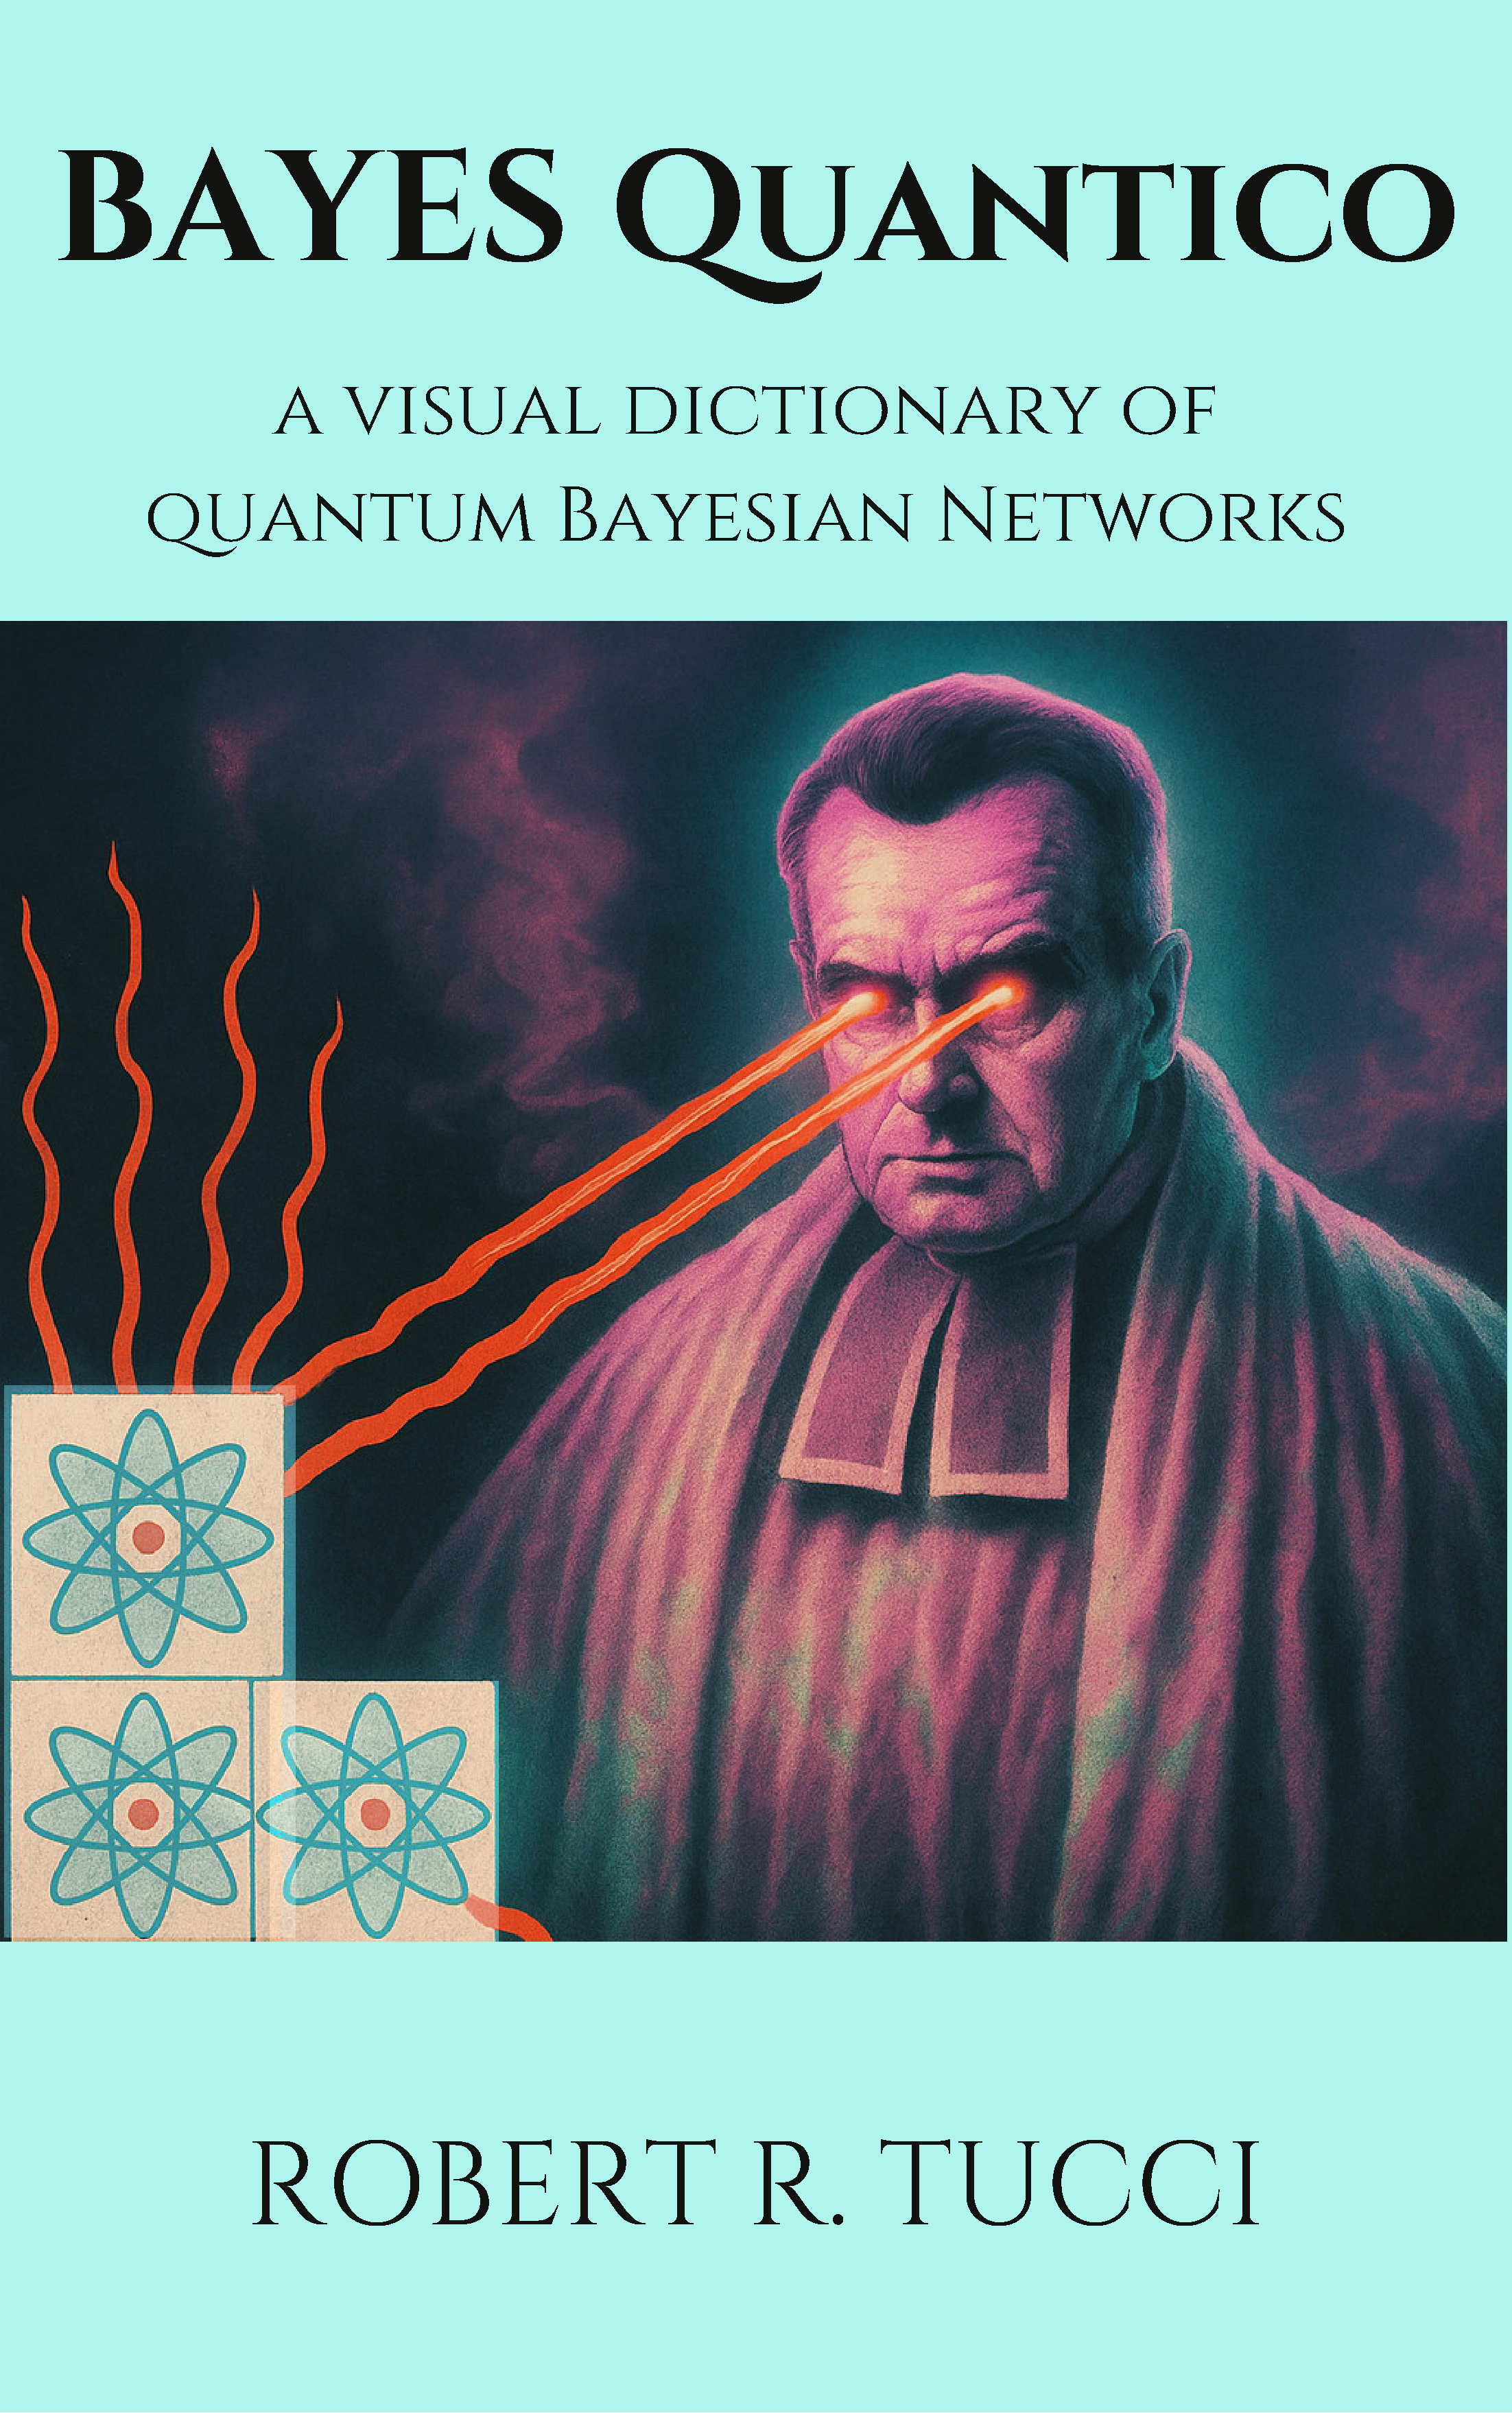
\includepdf[pages=-]{bayes-quantico-cover.pdf}
\maketitle
\newpage
\noindent
{\bf Bayesuvius Quantico}\\
by Robert R. Tucci\\
Copyright \copyright 2025, Robert R. Tucci.\\
\\
This work is licensed under the
Creative Commons Attribution-Noncommercial-No
Derivative Works 3.0 United States License.
 To view a copy of this license, visit the link
\url{https://creativecommons.org/licenses/by-nc-nd/3.0/}
or send a letter to Creative Commons,
 PO Box 1866, Mountain View, CA 94042.
\newpage



\newpage
\setcounter{tocdepth}{10}
\tableofcontents
\begin{appendices}
\chapter{Notational Conventions and Preliminaries}
\label{ch-conventions}
This book is a sequel to
my book entitled \qt{Bayesuvius}
(see Ref.\cite{bayesuvius}). 
For consistency, 
I have tried to follow in this book the 
same notational conventions
used in the prior book.
If any notation is not defined in this book,
check in the prior book. It might be
defined there.  

\section{Set notation}

The number of elements in any set $S$ is denoted by $|S|$.

$\ZZ$ = integers

$\ZZ_>0$ = positive integers

$\ZZ_{[a,b]} = a, a+1, \ldots, b$
for some integers $a, b$ such that $a\leq b$

$\RR$ = reals

$\CC$= complex numbers

$\CC^{n\times m}$ = $n\times m$ matrices of complex numbers

\section{Group}

A {\bf group}
$\calg$
is a set of elements
with a multiplication map $\calg\times \calg
\rarrow \calg$
such that


\begin{enumerate}
\item 
the multiplication is {\bf associative
}; i.e., 

\beq
(ab)c = a(bc)
\eeq
for $a,b,c\in\calg$.

\item
there exists an {\bf identity element}
$e\in \calg$
such that 

\beq
ea=ae=a
\eeq
for all $a\in \calg$

\item
for any $g\in\calg$,
there exists an {\bf inverse} $a^{-1}\in \calg$ such that

\beq
aa^{-1}=a^{-1}a=e
\eeq
\end{enumerate}

$|\calg|$ (i.e., number of
elements in $\calg$)
is called the {\bf order}
of the group.

If multiplication is
{\bf commutative}
(i.e., $ab=ba$ for all $a,b\in\calg$),
the group is said to be {\bf abelian}.

A {\bf subgroup} $\calh$ 
of $\calg$
is a subset of $\calg$
($\calh \subset \calg$)
which is also a group.
It's easy to show that any $\calh\subset \calg$ is a group if it
contains the identity
and is {\bf closed 
under multiplication} (i.e., $ab\in \calh$ for all $a,b\in \calh$) 



\section{Group  Representation}

A {\bf group representation} (rep)
of a group $\calg$
is a map $\phi: \calg\rarrow \CC^{n\times n}$\footnote{More generally, the $\CC^{n\times n}$ can be replaced by $\RR^{n\times n}$ or by $\FF^{n\times n}$ for any field $\FF$} such that

\beq
\phi(a)\phi(b)=
\phi(ab),
\quad \phi(e) = I
\eeq
where $e$ is the
identity of the group
and $I$ 
is the identity matrix.
Such a map is called a {\bf homomorphism}
(because it preserves an operation).
The map $\phi$ 
partitions $\calg$
into disjoints subsets (equivalence classes),
such that all elements of $\calg$ in each disjoint subset 
are represented by the same matrix.

One  way to specify a representation is
to give the effect of each group element $a\in \calg$ on a basis of vectors $\{\ket{1}, \ket{2}, \dots, \ket{n}\}$.


\beq
\phi (a)\ket{i}= \sum_j M_{ij}\ket{j}
\implies \av{i|\phi(a)|j} = M_{ij}
\eeq

If the map $\phi$
is 1-1, onto, we call it a {\bf faithful representation} 

The {\bf trivial representation} 
represents all $g\in \calg$
by  $diag(1,1, \dots, 1)$.
It's dimension is $d_\lam=0$.
It's not a faithful rep.

A {\bf singlet representation}
represents all
$g\in \calg$
by  $ z(g) diag(1,1, \dots, 1)$
for some $z(g)\in\CC$.
For the singlet rep, $\av{i|\phi(a)|j}=z(g)
\delta(i,j)$.
It's dimension is $d_\lam=1$.
The projection operator
$\delta_a^b \delta_c^d$
when acting on $G\indices{_c^d}$
gives a $ z(G) diag(1,1, \dots, 1)$
where $z(G)=\tr(G)$, so it
projects to a singlet rep.



When a group is 
defined using matrices, those
matrices are called the {\bf defining representation} (defrep). For example,
the group
of {\bf General Linear Transformations}
is defined by

\beq
GL(n, \CC)=
\{M\in \CC^{n\times n}: \det{M}\neq 0\}
\eeq

The {\bf adjoint representation} (adjrep)
is defined in terms of the structure constants
of the Lie Algebra. If the Lie Algebra satisfies
$[T^i, T^j]= if_{ijk}T^k$,
then the adjrep is given by the matrices 
with $i,j$ entries $M^k_{ij}=-if\indices{^k_i_j}$.
Write $\ket{T^i}$ instead of $T^i$
and  $\ket{x} = x_i \ket{T^i}$.
Then

\beq
[\ket{x}, \cdot]\ket{T^j}   = i f_{ijk}\ket{T^k} \implies
\bra{T^k}[\ket{x}, \cdot]\ket{T^j}= 
i x_i f_{ijk}
\eeq


{\bf Irreducible representations} (irreps)
are defined in Ch. \ref{ch-reducibility}

The {\bf fundamental representation} (funrep)
is defined as the smallest irrep.. 
The defrep equals the funrep for
$SU(n), SO(n), SP(n)$, but not for $E_8$.



\section{Group Theory References}
Much of this book
deals with Group Theory (GT).


GT is a vast subject. Who would have thought
that the simple definition of 
a group would generate so many elegant, highly applicable and useful results and
consequences.

GT books by mathematicians are very
different from GT
books by physicists,
even though, of course,
they agree on the definitions. 
Mathematicians
are, as to be expected, more rigorous and abstract. But it goes much further than that. Physicists are much
more interested in applications
to physical systems,
especially Quantum Mechanics (QM).
Soon after QM was invented,
it was realized that Linear Algebra (LA) and GT  (especially Group Representation Theory,
which combines GT and LA)
are extremely
relevant and useful in QM.
Hermann Weyl,
Eugene Wigner, Hans Bethe, Linus Pauling, etc.
combined QM and GT to understand the spectra and chemistry of atoms and molecules,
and later GT was heavily used in Quantum Field Theory and Particle Physics to devise 
the Standard Model. Condensed Matter physicists have also used it to understand crystalline solids and to devise quasi particles that can be detected in the lab. 

My PhD is in physics
so in this book I cover 
GT topics that are  mainly of interests to
physicists and engineers. Furthermore,
I am nowhere as abstract and
rigorous as mathematicians 
usually are.

My favorite books about GT 
for physicists are the Elliott \& Dawber's (ED)
2 volume series Ref. \cite{eli-daw-book}
and Predrag Cvitanovic's Birdtracks book
Ref.\cite{birdtracks-book}. I highly
recommend both of these references. I think
both of them are excellent.

The Birdtracks book explains key 
concepts in GT representation theory
using network diagrams 
(Cvitanovic calls 
such diagrams birdtracks) whereas the ED book doesn't use that type of diagram. Many people don't use birdtracks either, they only use algebra.
But since this is a book
about visualization using network diagrams (quantum 
bnets), we use birdtracks.
In fact, many
of the chapters in this
book were heavily influenced 
by Ref.\cite{birdtracks-book}
by Cvitanovic. I hope he doesn't mind. I really love his  book.

\section{Vector Space and Algebra over a field $\FF$}
\label{sec-algebra-over-f}

A vector  space
(a.k.a. linear space)  $\calv$
is defined as a set endowed with
two operations: vector addition $+:\calv\times\calv\rarrow \calv$,
and scalar multiplication $\FF\times\calv\rarrow \calv$,
such that

\begin{itemize}
\item $\calv$ is an abelian group under $+$
with identity $0$ and inverse of $x\in\calv$ equal to $-x\in\calv$

\item
For $\alp, \beta\in\FF$ and
$x,y\in\calv$
\beqa
\alp(x+y) &=& \alp x + \alp y
\\
(\alp +\beta)x &=& \alp x + \beta x
\\
\alp(\beta x)
&=&
(\alp\beta)x
\\
1x &=& x
\\
0x &=& 0
\eeqa
\end{itemize}
 In this book, we will always use either $\CC$ or $\RR$ for $\FF$. Both 
 of these fields are infinite but some fields are finite.


An {\bf algebra} $\cala$ is a
vector space  
which, 
besides being endowed with vector addition
and scalar multiplication
as all vector spaces are,
it has
a {\bf bilinear vector product}.
A bilinear vector product is a product that is linear on both sides; i.e., 

\beq
(\alp x + \beta y)\cdot z =
\alp x\cdot z +
\beta y\cdot z
\eeq
and 
\beq
z\cdot(\alp x + \beta y)=
\alp z \cdot x +
\beta z\cdot y
\eeq
for $x,y, z\in \cala$ and 
$\alp, \beta\in\CC$.
The cross product (but not the dot product)
for vectors in $\RR^3$,
the multiplication of 2 complex numbers, the product or commutator of 2
square matrices, are all good examples of
bilinear vector products.

Let $B = \{\tau_i: i=1, 2, \ldots, r\}$
be a basis for the vector space $\cala$. 
Then note that
$B$ is closed under vector multiplication. 

\beq
\tau_i\cdot \tau_j=
\sum_k c\indices{_{ij}^k} \tau_k
\eeq
where $c\indices{_{ij}^k}\in\CC$.
The $c\indices{_{ij}^k}$ are called 
{\bf structure constants} of $B$.

An {\bf associative algebra} satisfies 
$(x\cdot y)\cdot z = x\cdot(y\cdot z)$ for
$x,y,z\in \cala$.
\begin{itemize}
\item Not associative: cross product for vectors in  $\RR^3$.
\item Associative:
the product or commutator of 2  square matrices and the product of complex numbers
\end{itemize}

\section{Tensors}
\label{sec-tensors}
Let 

$(x_a)=(x_1, x_2, \ldots, x_n) = x^{:n}\in V^n=\CC^{n\times 1}$

Reverse of vector $rev(x_1, x_2, \ldots, x_n)=
(x_n, x_{n-1},
\ldots, x_1)$

$y^b = \sum_a g^{ba} x_a$

$(y^b)=(y^1, y^2, \ldots, y^n)= \dual{y}^{:n}\in \dual{V}^n=\CC^{n\times 1}$. $V^n$ is the lower indices vector space and
$\dual{V}^n$ is its {\bf dual vector space} (i.e., with upper indices).



$M\indices{_a^b}\in \CC^{n\times n}$, $a, b\in\ZZ_{[1,n]}$

Implicit Summation Convention

\beq
M\indices{_a^b}x_b = \sum_{b=1}^n
M\indices{_a^b}x_b
\eeq



If the Hermitian conjugate $\dagger$
equals $*T$ where $*$ is complex conjugation and $T$ is transpose,
then define

\beq
(M^\dagger)\indices{_b^a}= (M\indices{_a^b})^*,
\quad
(M^T)\indices{_b^a}= M\indices{_a^b},
\eeq
Thus, $\dagger$ and $T$ 
do two things: (1) reverse the horizontal order of the indices (2)
reverse vertical positions
of the indices; i.e., 
lower upper indices and raise lower indices.
Hermitian conjugation 
also complex conjugates the tensor components.

If $M$ is a Hermitian matrix (i.e., $M^\dagger =M$),

\beq
M\indices{^b_a}= (M\indices{_a^b})^*
\eeq



\begin{figure}[h!]
\centering
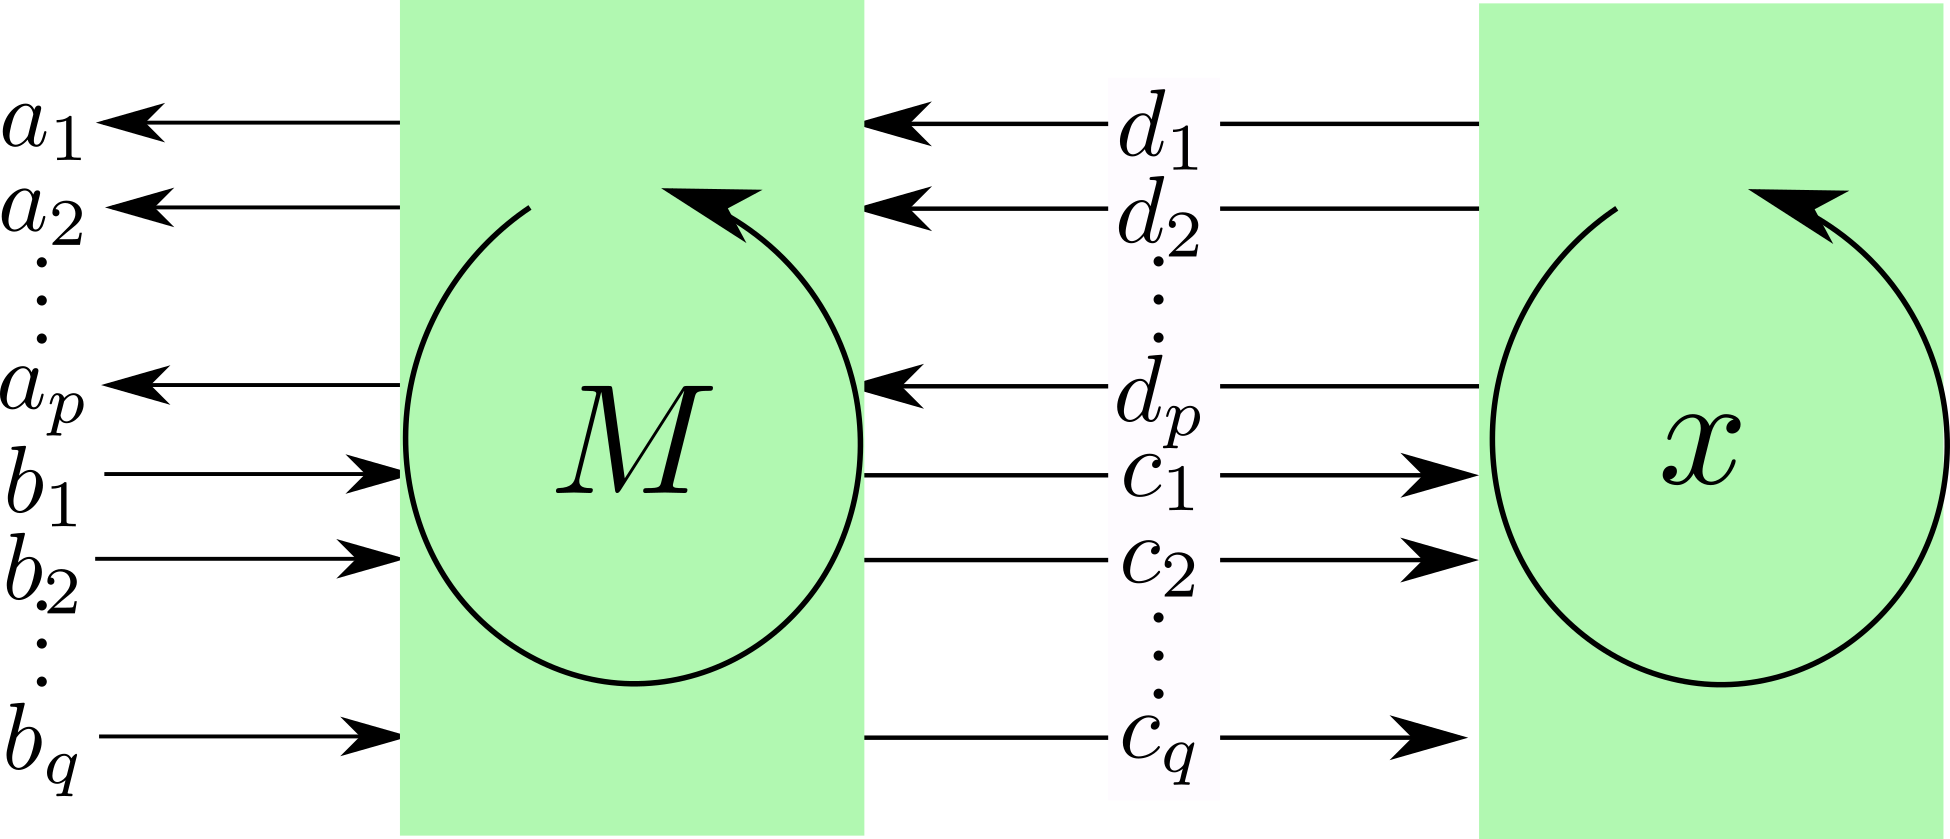
\includegraphics[width=2.7in]
{conventions/index-labels-Mx.png}
\caption{Index labels for $Mx$
where $M
\in \CC^{n^{p+q}\times n^{p+q}}$ and
$x\in V^{n^p}\otimes \dual{V}^{n^q}$.
Note that we  list indices in counterclockwise (CC) direction, 
starting at the top.}
\label{fig-index-labels-Mx}
\end{figure}

\begin{figure}[h!]
\centering
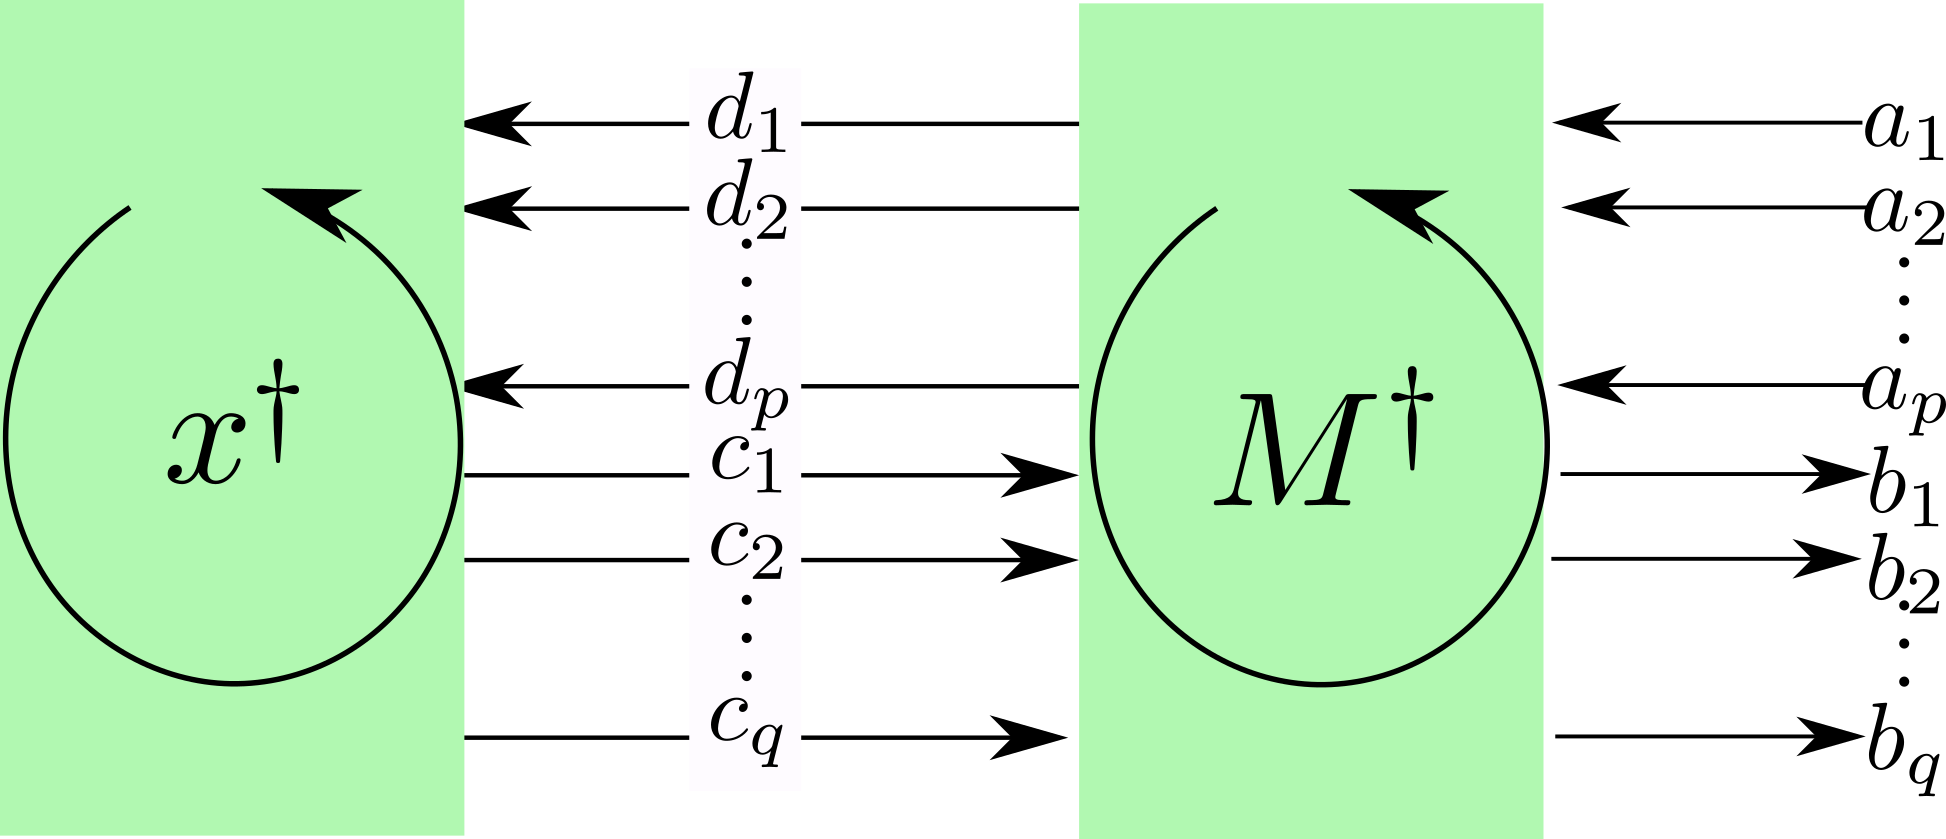
\includegraphics[width=2.7in]
{conventions/index-labels-hermitian.png}
\caption{Index labels for $x^\dagger M^\dagger$
corresponding to Fig.\ref{fig-index-labels-hermitian}.
Note that we  list indices in counterclockwise (CC) direction, 
starting at the top. }
\label{fig-index-labels-hermitian}
\end{figure}


Suppose $a_i, b_i, c_i, d_i\in \ZZ_{[1,n]}$.
From Fig.\ref{fig-index-labels-Mx}

\beq
y\indices{
_{a^{:p}}
^{b^{:q}}}=
M\indices{
_{a^{:p}}
^{b^{:q}}
_{rev(c^{:q})}
^{rev(d^{:p})}
}
x\indices{
_{d^{:p}}
^{c^{:q}}
}
\eeq
If we define $X_\alp$
and $x^\alp$ by

\beq
X\indices{_\alp} = X\indices{
_{a^{:p}}
^{b^{:q}}
}
,\quad
X\indices{^\alp}
=
X\indices{
_{rev(b^{:q})}
^{rev(a^{:p})}
}
\eeq
then

\beq
x_\alp = M\indices{_\alp^\beta}x_\beta
\eeq


\hrule

Hermitian conjugation (see Fig.\ref{fig-index-labels-hermitian})

\beq
\left\{
\begin{array}{l}
(M^\dagger)\indices{_a^d}=
(M\indices{_d^a})^*
\\
(M^\dagger)\indices{_\alp^{\delta}}=
(M\indices{
_{rev(\delta)}
^{rev(\alp)}
})^*
\end{array}\right.
\eeq
Note that
$\dagger$ does 3 things
to the birdtrack:

\begin{enumerate}
\item It flips the horizontal
axis of the figure. (In the
algebraic expression of the tensor, this
corresponds to
reversing the horizontal 
order of the indices.)

\item For each node, it changes incoming
arrows to outgoing ones and vice versa.
(In the
algebraic expression of the tensor, this
corresponds 
reversing the vertical
positions of the indices; i.e., 
lowering upper indices
and raising lower ones.)

\item
It replaces the tensor component
by its complex conjugate

\end{enumerate}


Hermitian matrix
 
\beq
M^\dagger
 = M,\quad
 \left\{
 \begin{array}{l}
(M\indices
{_d^a })^*
= M\indices{_a^d}
\\
(M\indices{_{rev(\delta)}^{rev(\alp)}})^*
=
M\indices{_\alp^{\delta}}
\end{array}
\right.
\eeq
Unitary matrix

\beq
M^\dagger
 M=1,\quad
 \left\{
 \begin{array}{l}
(M\indices
{_d^a })^*
M\indices{_a^d}=1
\\
(M\indices{_{rev(\delta)}^{rev(\alp)}})^*
M\indices{_\alp^{\delta}}=1
\end{array}
\right.
\eeq

\hrule

Note that
for $x\in V^n{}$, $y\in \dual{V}^n$, and $G\in \calg\subset GL(n, \CC)$,

\beq
(x')_a (y')^b= G\indices{^b_c} 
G\indices{_a^d}x_dy^c
\eeq


If $x\in V^{n^p}\otimes \dual{V}^{n^q}$, $\GG\in \calg\subset GL(n^{p+q}, \CC)$,

\beq
(x')\indices{
_{a^{:p}}
^{b^{:q}}
}
=
\GG\indices{
_{a^{:p}}
^{b^{:q}}
_{rev(c^{:q})}
^{rev(d^{:p})}
}
x\indices{
_{d^{:p}}
^{c^{:q}}
},
\quad
(x'_\alp=\GG\indices{_\alp^\beta}x_\beta)
\label{eq-xprime-eq-gg-x}
\eeq
where we define

\beq
\GG\indices{
_{a^{:p}}
^{b^{:q}}
_{rev(c^{:q})}
^{rev(d^{:p})}
}
\eqdef
\prod_{i=1}^p
G\indices{
_{a_i}
^{d_i}
}
\prod_{i=1}^q
\dual{G}\indices{
^{b_i}
_{c_i}
}
\eeq


\hrule
An issue that arises with tensors is this:
When is it permissible to represent 
a tensor by $M_{ab}^{cd}$?
If we define
$M_{ab}^{cd}$  by
\beq
M_{ab}^{cd} = M\indices{_a_b^c^d}
\eeq
then it's always permissible.
Then one can define
tensors like
$M\indices{_a^b^c^d}$
as 

\beq
M\indices{_a^b^c^d}=
g^{bb'}M\indices{_a_{b'}^c^d}
=
g^{bb'}M_{ab'}^{cd}
\eeq
Hence, one drawback of
using the notation
$M_{ab}^{cd}$
is that if one is interested 
in using versions of
$M_{ab}^{cd}$ with
some indices raised or 
lowered, one has to 
write down explicitly the metric tensors 
that do the lowering and
raising.
Instead of writing
$M\indices{_a^b^c^d}$,
you'll have to write
$g^{bb'}M_{ab'}^{cd}$.
This is not very onerous when 
explaining a topic
in which not much
lowering and raising of indices is
done. But in topics like
General Relativity that do
use a lot of raising and lowering of indices, it might not be 
too succinct.

\section{Permutations}
\label{sec-permutation-group}
Some well known notation 
and results about permutations are these.

$(1,2)$ stands for a {\bf transposition}; i.e., a map that swaps 1 and 2:


\beq\left(
\bcen
\footnotesize
\xymatrix@R=1pc@C=1pc{
1\ar[rd]
&2\ar[ld]
&3\ar[d]
&\ldots
&p\ar[d]
\\
1
&2
&3
&\ldots
&p
}
\ecen
\right)
\eeq

$(3,2,1)$ stands for a {\bf permutation}; i.e., a map that maps $3\rarrow 2\rarrow 1\rarrow 3$. 
\beq\left(
\bcen
\footnotesize
\xymatrix@R=1pc@C=1pc{
1\ar[rrd]
&2\ar[ld]
&3\ar[ld]
&4\ar[d]
&\ldots
&p\ar[d]
\\
1
&2
&3
&4
&\ldots
&p
}
\ecen
\right)
\eeq



Any
reordering of $(1,2,3,\ldots, p)$
is a permutation of $p$ letters (or numbers or elements).

The set $S_p$ of all permutation of
$p$ letters 
is called the {\bf symmetric group in $p$ letters}. It has $p!$ elements  (i.e., $|S_p|=p!$) and is a group,
where the group's product is map composition
and the group's identity element
is the identity map.

Any permutation can be expressed as a product of transpositions, For example,  $(3,2,1)=(3,2)(2,1)$.




An {\bf even permutation} such as
$(3,2,1)$ can be expressed as a product of an even number of 
transpositions. An {\bf odd permutation} can be expressed as a product of an odd
number of transpositions.
\chapter{Birdtracks}
\label{ch-birdtracks}

Cvitanovic Birdtracks book \cite{birdtracks-book}


Elliott-Dawber book \cite{eli-daw-book}

My paper \qt{Quantum Bayesian Nets} \cite{tucci-qbnets}

\section{Classical Bayesian Networks and their Instantiations}

TPM (Transition Probability Matrix) $P(y|x)\in [0,1]$
where  $x\in val(\rvx)$ and $y\in val(\rvy)$

\beq
\sum_{y\in val(\rvy)}P(y|x) = 1
\eeq

\beq
\calc=
\bcen
\xymatrix{
&\rvb\ar[ld]
\\
\rvc
&&\rva\ar[ll]\ar[lu]
}
\ecen
\eeq

\beq
\calc(a,b,c)
=
P(c|b,a)P(b|a)P(a)
=
\bcen
\xymatrix{
&b\ar[ld]
\\
c
&&a\ar[ll]\ar[lu]
}
\ecen
P(a)
\eeq

$a^{:2} = (a_1, a_2)$
\beq
\calc'=
\bcen
\xymatrix{
&\rvb\ar[ld]
\\
\rvc
&&\rva^{:2}\ar[ll]|{\rva_2}\ar[lu]|{\rva_1}
}
\ecen
\eeq

\beq
\calc'(a^{:2},b,c)
=
P(c|b,a_2)P(a_2|a^{:2})P(b|a_1)P(a_1|a^{:2})P(a^{:2}
)
=
\bcen
\xymatrix{
&b\ar[ld]
\\
c
&&a^{:2}
\ar[ll]|{a_2}\ar[lu]|{a_1}
}
\ecen
P(a^{:2})
\eeq

Marginalizer nodes  $\rva_1$ and $\rva_2$
have the TPMs
\beq \color{blue}
P(a'_i|\rva^{:2}=(a_1,a_2)) = \delta(a'_i, a_i)
\eeq
for $i=1,2$


\section{Quantum Bayesian Networks and
their Instantiations}

TPM (Transition Probability Matrix) 
$A(y|x)\in\CC$
where  $x\in val(\rvx)$ and $y\in val(\rvy)$

\beq
\sum_{y\in val(\rvy)}|A(y|x)|^2 = 1
\label{eq-bnet-normalization}
\eeq
Note that if $A$ is the matrix with entries
$\av{y|A|x}=A(y|x)$, then

\beq
\av{y|A^\dagger A|x}=\sum_{y\in val(\rvy)}|A(y|x)|^2 = 1
\eeq
If $A$ is a unitary matrix, then $A^\dagger A= AA^\dagger =1$ so this
Eq.(\ref{eq-bnet-normalization})
is satisfied.

\beq
\calq=
\bcen
\xymatrix{
&\rvb\ar[ld]
\\
\rvc
&&\rva\ar[ll]\ar[lu]
}
\ecen
\eeq

\beq
\calq(a,b,c)
=
A(c|b,a)A(b|a)A(a)
=
\bcen
\xymatrix{
&b\ar[ld]
\\
c
&&a\ar[ll]\ar[lu]
}
\ecen
A(a)
\eeq

$a^{:2} = (a_1, a_2)$
\beq
\calq'=
\bcen
\xymatrix{
&\rvb\ar[ld]
\\
\rvc
&&\rva^{:2}\ar[ll]|{\rva_2}\ar[lu]|{\rva_1}
}
\ecen
\eeq

\beq
\calq'(a^{:2},b,c)
=
A(c|b,a_2)A(a_2|a^{:2})A(b|a_1)A(a_1|a^{:2})A(a^{:2})
=
\bcen
\xymatrix{
&b\ar[ld]
\\
c
&&a^{:2}
\ar[ll]|{a_2}\ar[lu]|{a_1}
}
\ecen
A(a^{:2})
\eeq

Marginalizer nodes  $\rva_1$ and $\rva_2$
have the TAMs
\beq \color{blue}
A(a'_i|\rva^{:2}=(a_1,a_2)) = \delta(a'_i, a_i)
\eeq
for $i=1,2$

\section{Birdtracks}



\beq
\delta(b,a)=\indi(a=b)=
\delta^b_a =
\xymatrix{a&\ar[l]|\bullet b}
\eeq


\beq
\bra{a,b}
X\indices{_\rva_\rvb^\rvc^\rvd}
\ket{c,d}
=
X\indices{_a_b^c^d}
=
\bcen
\xymatrix@R=1pc{
\rva=a
&X\indices{_\rva_\rvb^\rvc^\rvd}
\ar[dl]\ar[l]
\\
\rvb=b
\\
\rvc=c\ar[ruu]
\\
\rvd=d\ar[ruuu]
}\ecen
\eeq

\beq
\bcen
\xymatrix@R=1pc{
a
&X\indices{_\rva_\rvb^\rvc^\rvd}
\ar[dl]\ar[l]
\\
b
\\
c\ar[ruu]
\\
d\ar[ruuu]
}\ecen
\rarrow
\bcen
\xymatrix@R=1pc{
a,b
&X\indices{_\rva_\rvb^\rvc^\rvd}
\ar[dl]\ar[l]
\\
a,b
\\
c\ar[ruu]
\\
d\ar[ruuu]
}\ecen
\eeq
$X\indices{_\rva_\rvb^\rvc^\rvd}\in V^2 \otimes V_2$.
Sometimes, 
we will omit denote
this node simply by $X$.
This if okay as long as
we are not using,
$X$ to also denote
a different version of $X\indices{_\rva_\rvb^\rvc^\rvd}$
with some of the indices
raised or lowered or 
their order has been changed.
\footnote{For matrices,
$(A^\dagger)_{i,j} = (A_{j, i})^*$
so
taking a Hermitian conjugate
involves both taking
the complex conjugate of
the matrix element and reversing the left-to-right (L2R) order of its indices.
This generalizes to 
$(X^\dagger)\indices{_d_c^b^a}=
(X\indices{_a_b^c^d})^*$.
Besides raising and lowering indices, we reverse their L2R order.
}

\beq
(X^\dagger)\indices{_d_c^b^a}
=
\bcen
\xymatrix@R=1pc{
(X^\dagger)\indices{_\rvd_\rvc^\rvb^\rva}
&\rva=a\ar[l]
\\
&\rvb=b\ar[lu]
\\
&\rvc=c\ar[luu]
\\
&\rvd=d\ar[luuu]
}\ecen
\eeq


\beqa
(X^\dagger)\indices{_d_c^b^a}
X\indices{_a_b^c^d}
&=&
\bcen
\xymatrix@R=1pc{
(X^\dagger)\indices{_\rvd_\rvc^\rvb^\rva}
&\sum a\ar[l]\ar@{<-}[r]
&
X\indices{_\rva_\rvb^\rvc^\rvd}
\\
&\sum b\ar[ul]\ar@{<-}[ur]
&
\\
&\sum c\ar@{<-}[luu]
\ar[ruu]
&
\\
&\sum d\ar@{<-}[luuu]
\ar[ruuu]
&
}
\ecen
\\
&=&
\bcen
\xymatrix@R=1pc{
X^\dagger
&\ar[l]\ar@{<-}[r]
&
X
\\
&\ar[ul]\ar@{<-}[ur]
&
\\
&\ar@{<-}[luu]
\ar[ruu]
&
\\
&\ar@{<-}[luuu]
\ar[ruuu]
&
}
\ecen
\eeqa

Birdtracks originated as a graphical
way to represent the tensors in General Relativity (Gravitation). In General Relativity, one deals with tensors such as
$T\indices{_a^b_c}$ which have some indices raised
and some lowered. One can use the metric 
$g^{a,b}$ to raise all the lowered indices
to get $T^{abc}$. If we represent this
graphically as a node with incoming arrows 
$a,b,c$, we need to 
follow one of the following
2 conventions: either
\begin{enumerate}
\item
label the arrows 
as $\rva$, $\rvb, \rvc$, 
and define the node as
$T^{\rva\rvb\rvc}$,
or
\item
instead of labelling the
arrows explicitly $\rva, \rvb, \rvc$, 
 indicate in the node
where is the first arrow
$\rva$, and draw the
arrows $\rva, \rvb, \rvc$
so that they enter the node
in {\bf counterclockwise} (CC) order.
The {\bf left-to-right} (L2R) order
of the indices on $T$ corresponds
the CC order of the arrows.
\end{enumerate}
If we don't do either 1 or 2, we won't
be able to distinguish between
the graphical
representations of $T^{1,2,3}$
and $T^{2,1,3}$, for example.
Cvitanovic's Birdtracks book
Ref.\cite{birdtracks-book} follows Convention 2, but
most of the time, in this book, we will follow
Convention 1 \footnote{If we follow Convention 1,
we don't need to reverse the L2R order of the indices
when taking a Hermitian conjugate. Thus,
$(X^\dagger)\indices{^\rva^\rvb_\rvc_\rvd}=
X\indices{_\rva_\rvb^\rvc^\rvd}=
X\indices{^\rvd^\rvc_\rvb_\rva}$.
As long as $\rva, \rvb$ are lower indices and $\rvc,\rvd$ are upper
indices of $X$, any L2R
order of $\rva, \rvb, \rvc, \rvd$ 
is equivalent
under Convention 1.}
The reason I chose to do so is for the sake of consistency:
Convention 2 
is closer to the quantum bnet conventions. 





$a^{:m}\in \ZZ_+^m$

\beq
R^{a_3^{:m_3}, b_2^{:n_2}}
_{b_3^{:n_3}, a_2^{:m_2}}
S^{a_2^{:m_2}, b_1^{:n_1}}
_{b_2^{:n_2}, a_1^{:m_1}} =
\bcen
\xymatrix{
b_3^{:n_3}
&R\ar[l]\ar@{<-}[ld]
&\sum  b_2^{:n_2}\ar[l]
&S\ar[l]\ar@{<-}[ld]
&b_1^{:n_1}\ar[l]
\\
a_3^{:m_3}
&
&\sum a_2^{:m_2}\ar@{<-}[lu]
&
&a_1^{:m_1}\ar@{<-}[lu]
}
\ecen
\eeq

\beq
\tr_\rvb X\indices{_a_\rvb^\rvb^d}
=
\sum_b X\indices{_a_b^b^d}
=
\bcen
\xymatrix@R=1pc{
a
&X\indices{_\rva_\rvb^\rvc^\rvd}
\ar[dl]\ar[l]
\\
\ar@[red]@{-}[d]
&
\\
\ar[ruu]
\\
d\ar[ruuu]
}\ecen
\eeq


\beq
\xymatrix{
&\ar[d]
&
&\ar@{<-}[d]\ar@[red]@{-}[ll]
&
\\
&R\ar[l]\ar@{<-}[ld]
&
&S\ar@{<-}[ld]
&\ar[l]
\\
&
&\ar@{<-}[lu]
&
&\ar@{<-}[lu]
}
\eeq
\end{appendices}
\chapter{Casimir Operators}
\label{ch-casimir}

\beq
M_2 = 
\xymatrix{
&\ar[l]T_i&
\ar@{~}@/_1.5pc/[l]\ar[l]
T_i
&\ar[l]
}
\eeq

\beq
M_4 = 
\bcen
\xymatrix@C=1pc{
\ar[r]
&T_i\ar@{~}[d]\ar[r]
&T_j\ar@{~}[d]\ar[r]
&T_k\ar@{~}[dr]\ar[r]
&T_l\ar@{~}[dl]\ar[r]
&\ar@/_1.5pc/@[red][lllll]
\\
&T_i\ar[l]
&T_j\ar[l]
&T_l\ar[l]
&T_k\ar[l]
&\ar[l]
}
\ecen
\eeq

\begin{align}
0 &= [T_r, M]
\\
&=
\bcen
\xymatrix@C=1pc{
&
&\ar[r]
&T_i\ar@{~}[d]\ar[r]
&T_j\ar@{~}[d]\ar[r]
&T_k\ar@{~}[dr]\ar[r]
&T_l\ar@{~}[dl]\ar[r]
&\ar@/_1.5pc/@[red][lllll]
\\
&T_r\ar@{~}[u]\ar[l]
&
&T_i\ar[ll]
&T_j\ar[l]
&T_l\ar[l]
&T_k\ar[l]
&\ar[l]
}
\ecen
-
\bcen
\xymatrix@C=1pc{
\ar[r]
&T_i\ar@{~}[d]\ar[r]
&T_j\ar@{~}[d]\ar[r]
&T_k\ar@{~}[dr]\ar[r]
&T_l\ar@{~}[dl]\ar[r]
&\ar@/_1.5pc/@[red][lllll]
&&
\\
&T_i\ar[l]
&T_j\ar[l]
&T_l\ar[l]
&T_k\ar[l]
&
&T_r\ar[ll]
\ar@{~}[u]
&\ar[l]
}
\ecen
\end{align}


\beq
M_2 M_4 = M_4 M_2
\eeq

\beq
\tr(T_i T_j \ldots T_l)
= \bcen
\xymatrix@C=1pc{
\ar[r]
&T_i\ar@{~}[d]\ar[r]
&T_j\ar@{~}[d]\ar[r]
&\ldots\ar[r]
&T_l\ar@{~}[d]\ar[r]
&\ar@/_1.5pc/@[red][lllll]
\\
&&&&&
}
\ecen
\eeq

\beq
\bcen
\xymatrix@C=1pc{
\ar[r]
&T_i\ar@{~}[d]\ar[r]
&T_j\ar@{~}[d]\ar[r]
&\ldots\ar[r]
&T_l\ar@{~}[d]\ar[r]
&\ar@/_1.5pc/@[red][lllll]
\\
&&&&&
}
\ecen
-
\bcen
\xymatrix@C=1pc{
\ar[r]
&T_j\ar@{~}[dr]\ar[r]
&T_i\ar@{~}[dl]\ar[r]
&\ldots\ar[r]
&T_l\ar@{~}[d]\ar[r]
&\ar@/_1.5pc/@[red][lllll]
\\
&&&&&
}
\ecen=
\bcen
\xymatrix@C=1pc{
\ar[r]
&T_k\ar@{~}@[green][d]\ar[r]
&\ldots\ar[r]
&T_l\ar@{~}[d]\ar[r]
&\ar@/_1.5pc/@[red][llll]
\\
&if\ar@{-}[dl]
\ar@{-}[dr]&&&&
\\
&&&
}
\ecen
\eeq

\beq
h_{i_1 i_2\ldots  i_p}
=
\frac{1}{p!}
\sum_{\s  \in \cals_p}
\tr(T_{\s(i_1)} T_{\s(i_2)} \ldots T_{\s(i_p)})
= \bcen
\xymatrix@C=1pc{
\ar[r]
&T_{i_1}\ar@{~}[d]\ar[r]
&T_{i_2}\ar@{~}[d]\ar[r]
&\ldots\ar[r]
&T_{i_p}\ar@{~}[d]\ar[r]
&\ar@/_1.5pc/@[red][lllll]
\\
&\ar@{~}[d]
&\ar@{~}[d]
&
&\cals_p\ar@2{-}[lll]
\ar@{~}[d]
&
\\
&
&
&
&
}
\ecen
\eeq

\beq
d_{ijk}=
\bcen
\xymatrix@R=1pc{
i&&
\\
&d
\ar@{~}`u[ul][ul]
\ar@{~}`d[dl][dl]
&\ar@{~}[l]k
\\
j&&
}
\ecen
=
2
\bcen
\xymatrix@R=1pc{
i&\cals_2\ar@{~}[l]
\ar@2{-}[dd]
&\ar@{~}[l]
\ar[dd]&
\\
&&&\ar[ul]&k\ar@{~}[l]
\\
j&\ar@{~}[l]&\ar[ur]
\ar@{~}[l]&
}
\ecen
\eeq
Multiplying Jacobi identity by $T_k$
and taking the trace, we get

\beq
if_{ijk}=
\bcen
\xymatrix@R=1pc{
i&&
\\
&if
\ar@{~}`u[ul][ul]
\ar@{~}`d[dl][dl]
&\ar@{~}[l]k
\\
j&&
}
\ecen
=
2
\bcen
\xymatrix@R=1pc{
i&\cala_2\ar@{~}[l]
\ar@2{-}[dd]
&\ar@{~}[l]
\ar[dd]&
\\
&&&\ar[ul]&k\ar@{~}[l]
\\
j&\ar@{~}[l]&\ar[ur]
\ar@{~}[l]&
}
\ecen
\eeq

\section{Independent Casimirs of Simple Groups}




\beq
\myboxed{
M =\sum_i  T_i x_i}
\quad
\xymatrix{
&M\ar[l]&\ar[l]
}
=
\sum_i x_i
\bcen
\xymatrix{
&&
\\
a&\ar[l] T_i
\ar@{~}[u]
&\ar[l]b
}
\ecen
\eeq

\beqa
\tr(M^k)
&=&
\xymatrix@C=1pc{
&M\ar[l]
&M\ar[l]
&\ldots
&M\ar[l]
&\ar[l]
\ar@[red]@{-}@/_1pc/[lllll]
}
\\
\nonumber
\\
&=&
\sum_{i_1 i_2 \ldots i_k}
\bcen
\xymatrix@C=1pc{
&T_{i_1}\ar[l]\ar@{~}[d]
&T_{i_2}\ar[l]\ar@{~}[d]
&\ldots
&T_{i_k}\ar[l]\ar@{~}[d]
&\ar[l]
\ar@[red]@{-}@/_1pc/[lllll]
\\
&&&&
}
\ecen
x_{i_1}
x_{i_2}
\ldots
x_{i_k}
\\
&=&
\sum_{i_1 i_2 \ldots i_k}
\bcen
\underbrace
{\xymatrix@C=1pc{
&T_{i'_1}\ar[l]\ar@{~}[d]
&T_{i'_2}\ar[l]\ar@{~}[d]
&\ldots
&T_{i'_k}\ar[l]\ar@{~}[d]
&\ar[l]
\ar@[red]@{-}@/_1pc/[lllll]
\\
&&&&\ar@2{-}[lll]
\cals_k
\\
&\ar@{~}[u] i_1
&\ar@{~}[u]i_2
&
&\ar@{~}[u]i_{k}
}}_{h_{i_1 i_2 \ldots i_k}}
\ecen
x_{i_1}
x_{i_2}
\ldots
x_{i_k}
\eeqa

Recall Eq.(\ref{eq-char-eq-gen}) for
the general characteristic equation of a matrix $M$

\beqa
0&=&
\sum_{k=0}^n
(-1)^k \left(
\tr_{1\ldots n-k}
\cala_{n-k}
M^{\otimes n-k}
\right)
M^k
\\
&=&
\left\{
\begin{array}{l}
M^n
\\
- M^{n-1}(\tr M)
\\
+M^{n-2}
(\tr_{1\ldots 2}
\cala_2 M^{\otimes 2})
\\
\ldots
\\
(-1)^n det(M)
\end{array}
\right.
\eeqa

The coefficients of $M^k$ are products of traces of a single $T_i$. If we calculate 
the trace of $M^k$,
then that will entail
calculating traces with $k$ matrices $T_i$.

\begin{table}[h!]
\begin{tabular}{|
>{\columncolor[HTML]{FFFFC7}}l |l|}
\hline
$A_r = \mathfrak{su}(r+1)$ & $2,3, \ldots, r+1$ \\ \hline
$B_r = \mathfrak{so}(2r+1)$ & $2,4,6, \ldots, 2r$ \\ \hline
$C_r=\mathfrak{sp}(2r)$ & $2,4,6, \ldots, 2r$ \\ \hline
$D_r=\mathfrak {so}(2r)$ & $2,4,\ldots, 2r-2, 2r$ \\ \hline
$G_2$ & $2,6$ \\ \hline
$F_4$ & $2,6,8,12$ \\ \hline
$E_6$ & $2,5,6,8,9,12$ \\ \hline
$E_7$ & $6,8,10,12,14,18$ \\ \hline
$E_8$ & $8,12,14,18,20,24,30$ \\ \hline
\end{tabular}
\caption{Betti numbers for the simple Lie Algebras}
\label{tab-betti}
\end{table}

Betti number of a Casimir is the number
of $T_i$ being traced over (i.e., in the loop). Note that the Betti numbers are
all even except for
$SU(n)$.

For all Simple Lie Groups except for
$SU(n)$,
there is a invertible symmetric or
skew-symmetric 
bilinear invariant matrix $g_{ab}$ 
satisfying
$g_{ab}G^{bc}=\delta_a^c$. Hence


\beq
\bcen\xymatrix@C=1.3pc@R=1pc{
&g\ar@{<-}[d]
\\
&g\ar[d]
\\
&T_{i_2}\ar@{~}[l]\ar[d]
\\
&T_{i_3}\ar@{~}[l]\ar[d]
\\
&T_{i_4}\ar@{~}[l]\ar[d]
\\
&T_{i_5}\ar@{~}[l]\ar[d]
\\
&\ar@[red]@/_1.3pc/[uuuuuu]
}
\ecen
= (-1)
\bcen\xymatrix@C=1.3pc@R=1pc{
&g\ar@{<-}[d]
\\
&T_{i_1}\ar@{~}[l]\ar@{<-}[d]
\\
&g\ar[d]
\\
&T_{i_3}\ar@{~}[l]\ar[d]
\\
&T_{i_4}\ar@{~}[l]\ar[d]
\\
&T_{i_5}\ar@{~}[l]\ar[d]
\\
&\ar@[red]@/_1.3pc/[uuuuuu]
}
\ecen
= (-1)^2
\bcen\xymatrix@C=1.3pc@R=1pc{
&g\ar@{<-}[d]
\\
&T_{i_1}\ar@{~}[l]\ar@{<-}[d]
\\
&T_{i_2}\ar@{~}[l]\ar@{<-}[d]
\\
&g\ar[d]
\\
&T_{i_4}\ar@{~}[l]\ar[d]
\\
&T_{i_5}\ar@{~}[l]\ar[d]
\\
&\ar@[red]@/_1.3pc/[uuuuuu]
}
\ecen
= (-1)^3
\bcen\xymatrix@C=1.3pc@R=1pc{
&g\ar@{<-}[d]
\\
&T_{i_1}\ar@{~}[l]\ar@{<-}[d]
\\
&T_{i_2}\ar@{~}[l]\ar@{<-}[d]
\\
&T_{i_3}\ar@{~}[l]\ar@{<-}[d]
\\
&g\ar[d]
\\
&T_{i_5}\ar@{~}[l]\ar[d]
\\
&\ar@[red]@/_1.3pc/[uuuuuu]
}
\ecen
= (-1)^4
\bcen\xymatrix@C=1.3pc@R=1pc{
&g\ar[d]
\\
&T_{i_1}\ar@{~}[l]\ar@{<-}[d]
\\
&T_{i_2}\ar@{~}[l]\ar@{<-}[d]
\\
&T_{i_3}\ar@{~}[l]\ar@{<-}[d]
\\
&T_{i_4}\ar@{~}[l]\ar@{<-}[d]
\\
&g\ar[d]
\\
&\ar@[red]@/_1.3pc/[uuuuuu]
}
\ecen
\eeq

In general, a Casimir with $k$ $T_i$
equals itself times $(-1)^k$.
So only Casimirs with even $k$
are non-zero.


\begin{claim}
The following are a complete set
of Casimir operators for the given Groups
\beq
\begin{array}{lllll}
GL(n, \CC):
\\
\bcen
\xymatrix@C=.7pc{
&T_i\ar[l]&\ar[l]
\ar@{-}@[red]@/_1pc/[ll]
\\
&\ar@{~}[u]
}
\ecen
,
&
\bcen
\xymatrix@C=.7pc{
&T_i\ar[l]&T_j\ar[l]&\ar[l]
\ar@{-}@[red]@/_1pc/[lll]
\\
&\ar@{~}[u]&\ar@{~}[u]
}
\ecen
,
&
\bcen
\xymatrix@C=.7pc{
&T_i\ar[l]&T_j\ar[l]&T_k\ar[l]
&\ar[l]
\ar@{-}@[red]@/_1pc/[llll]
\\
&\ar@{~}[u]&\ar@{~}[u]&\ar@{~}[u]
\cals_3\ar@2{-}[ll]
\\
&\ar@{~}[u]&\ar@{~}[u]&\ar@{~}[u]
}
\ecen
,
&
\ldots
&
\bcen
\xymatrix@C=.7pc{
&T_{i_1}\ar[l]&T_{i_2}\ar[l]&\ldots\ar[l]&T_{i_n}\ar[l]
&\ar[l]
\ar@{-}@[red]@/_1pc/[lllll]
\\
&\ar@{~}[u]&\ar@{~}[u]&&\ar@{~}[u]
\cals_n\ar@2{-}[lll]
\\
&\ar@{~}[u]&\ar@{~}[u]&\dots&\ar@{~}[u]
}
\ecen

\end{array}
\eeq

\beq
\begin{array}{lllll}
SU(n):
\\
\bcen
\xymatrix@C=.7pc{
&T_i\ar[l]&T_j\ar[l]&\ar[l]
\ar@{-}@[red]@/_1pc/[lll]
\\
&\ar@{~}[u]&\ar@{~}[u]
}
\ecen
,
&
\bcen
\xymatrix@C=.7pc{
&T_i\ar[l]&T_j\ar[l]&T_k\ar[l]
&\ar[l]
\ar@{-}@[red]@/_1pc/[llll]
\\
&\ar@{~}[u]&\ar@{~}[u]&\ar@{~}[u]
\cals_3\ar@2{-}[ll]
\\
&\ar@{~}[u]&\ar@{~}[u]&\ar@{~}[u]
}
\ecen
,
&
\ldots
&
\bcen
\xymatrix@C=.7pc{
&T_{i_1}\ar[l]&T_{i_2}\ar[l]&\ldots\ar[l]&T_{i_n}\ar[l]
&\ar[l]
\ar@{-}@[red]@/_1pc/[lllll]
\\
&\ar@{~}[u]&\ar@{~}[u]&&\ar@{~}[u]
\cals_n\ar@2{-}[lll]
\\
&\ar@{~}[u]&\ar@{~}[u]&\dots&\ar@{~}[u]
}
\ecen

\end{array}
\eeq

\beq
\begin{array}{lllll}
SO(2r+1) \text{ and } Sp(2r):
\\
\bcen
\xymatrix@C=.7pc{
&T_i\ar[l]&T_j\ar[l]&\ar[l]
\ar@{-}@[red]@/_1pc/[lll]
\\
&\ar@{~}[u]&\ar@{~}[u]
}
\ecen
,
&
\bcen
\xymatrix@C=.7pc{
&T_{i}\ar[l]&T_j\ar[l]&T_k\ar[l]
&T_l\ar[l]&\ar[l]
\ar@{-}@[red]@/_1pc/[lllll]
\\
&\ar@{~}[u]&\ar@{~}[u]&\ar@{~}[u]&\ar@{~}[u]
\cals_4\ar@2{-}[lll]
\\
&\ar@{~}[u]&\ar@{~}[u]&\ar@{~}[u]&\ar@{~}[u]
}
\ecen
,
&
\ldots
&
\bcen
\xymatrix@C=.7pc{
&T_{i_1}\ar[l]&T_{i_2}\ar[l]&\ldots\ar[l]&T_{i_{2r}}\ar[l]
&\ar[l]
\ar@{-}@[red]@/_1pc/[lllll]
\\
&\ar@{~}[u]&\ar@{~}[u]&&\ar@{~}[u]
\cals_{2r}\ar@2{-}[lll]
\\
&\ar@{~}[u]&\ar@{~}[u]&\dots&\ar@{~}[u]
}
\ecen

\end{array}
\eeq

\beq
\begin{array}{c}
\begin{array}{lllll}
SO(2r):
\\
\bcen
\xymatrix@C=.7pc{
&T_i\ar[l]&T_j\ar[l]&\ar[l]
\ar@{-}@[red]@/_1pc/[lll]
\\
&\ar@{~}[u]&\ar@{~}[u]
}
\ecen
,
&
\bcen
\xymatrix@C=.7pc{
&T_{i}\ar[l]&T_j\ar[l]&T_k\ar[l]
&T_l\ar[l]&\ar[l]
\ar@{-}@[red]@/_1pc/[lllll]
\\
&\ar@{~}[u]&\ar@{~}[u]&\ar@{~}[u]&\ar@{~}[u]
\cals_4\ar@2{-}[lll]
\\
&\ar@{~}[u]&\ar@{~}[u]&\ar@{~}[u]&\ar@{~}[u]
}
\ecen
,
&
\ldots
&
\bcen
\xymatrix@C=.7pc{
&T_{i_1}\ar[l]&T_{i_2}\ar[l]&\ldots\ar[l]&T_{i_{2r-2}}\ar[l]
&\ar[l]
\ar@{-}@[red]@/_1pc/[lllll]
\\
&\ar@{~}[u]&\ar@{~}[u]&&\ar@{~}[u]
\cals_{2r-2}\ar@2{-}[lll]
\\
&\ar@{~}[u]&\ar@{~}[u]&\dots&\ar@{~}[u]
}
\ecen
\end{array}
\\
\bcen
\xymatrix@C=1pc@R=1pc{
\ar@{<-}[dr]
&
&\ar[dl]
&\ar@{<-}[dr]
&
&\ar[dl]
&
&\ar@{<-}[dr]
&
&\ar[dl]
\ar@2{-}[lllllllll]\cala^{\frac{1}{2}}_{2r}
\\
&\ar@{~}[d] T_{i_1}
&
&
&\ar@{~}[d] T_{i_2}
&
&
&
&\ar@{~}[d] T_{i_{r}}
&
\\
&&&&&&\ldots&&
}
\ecen
\end{array}
\eeq
\end{claim}
\proof
\beq
I_r(x)=
\bcen
\xymatrix@R=.7pc@C=1.3pc{
&\ar@2{-}[ddddddddd]\cala^{\frac{1}{2}}_{2r}
\\
M\ar[ur]&
\\
&\ar[ul]
\\
&
\\
M\ar[ur]&
\\
&\ar[ul]
\\
\ldots&
\\
&
\\
M\ar[ur]&
\\
&\ar[ul]
}
\ecen
\eeq

\beq
I_r^2(x)=
\bcen
\xymatrix@R=.7pc@C=1.3pc{
&\ar@2{-}[ddddddddd]\cala_{2r}
\ar[rd]&
\\
M\ar[ur]&&M\ar[ld]
\\
&\ar[ul]&
\\
&\ar[rd]&
\\
M\ar[ur]&&M\ar[ld]
\\
&\ar[ul]&
\\
\ldots&&
\\
&\ar[rd]&
\\
M\ar[ur]&&M\ar[ld]
\\
&\ar[ul]&
}
\ecen
=
\tr(M^{2r}) +\ldots
\eeq
\qed

\beqa
(I_p)\indices{_a^b}
&=&
\tr(
T_\lam^{i_1}
T_\lam^{i_2}
\ldots
T_\lam^{i_p}
)
(
T_\mu^{i_1}
T_\mu^{i_2}
\ldots
T_\mu^{i_p}
)\indices{_a^b}
\\
&=&
\bcen
\xymatrix@C=1pc@C=1pc{
\ar[r]
&
T^{i_1}_\lam\ar[r]
\ar@{~}[d]
&T^{i_1}_\lam\ar[r]
\ar@{~}[d]
&\ldots\ar[r]
&T^{i_p}_\lam
\ar@{~}[d]
&\ar[l]
\ar@[red]@/_1pc/@{-}[lllll]
\\
a&
T^{i_1}_\mu\ar[l]
&T^{i_1}_\mu\ar[l]
&\ldots\ar[l]
&T^{i_p}_\mu\ar[l]
&\ar[l]b
}
\ecen
\eeqa

\beq
M=
\bcen
\xymatrix{
\ar[r]&\ar[r]
T^i_\lam\ar@{~}[d]
&
\\
&\ar[l]T^i_\mu
&\ar[l]
}
\ecen
\eeq

\beqa
M &=& \sum_\rho
\bcen
\xymatrix@C=2pc@R=1pc{
\ar[rd]|\lam&&&\ar[rd]|\lam
T_\lam
\ar@{~}[dd]&&&
\\
&C^\dagger_\rho
\ar[ld]|\mu&
C_\rho\ar[ru]|\lam
\ar[l]|\rho\ar[ru]&&C^\dagger_\rho
\ar[ld]|\mu
&C_\rho\ar[l]|\rho\ar[ru]|\lam&
\\
&&&\ar[lu]|\mu
T_\mu&&&\ar[lu]|\mu
}
\ecen
\\
&=&
\sum_\rho
A(\lam,\rho,\mu)
\bcen
\xymatrix{
\ar[dr]|\lam&&&
\\
&C^\dagger_\rho\ar[dl]|\mu&\ar[l]|\rho C_\rho\ar[ru]|\lam&
\\
&&&\ar[lu]|\mu
}
\ecen
\eeqa


\beq
A(\lam,\rho,\mu)=
\frac{1}{d_\rho}
\bcen
\xymatrix@R=2pc@C=2pc{
&T_{\lam}^\dagger\ar@{~}[d]|{}
\ar@/_1pc/[ddl]|{\lam}
\ar@/^1pc/@{<-}[ddr]|{\lam}
\\
&T_{\mu}
\ar[dl]|{\mu}
\ar@{<-}[dr]|{\mu}
\\
T_{\rho}
&
&T_{\rho}^\dagger
\ar@{<-}[ll]|{\rho}
}
\ecen
\eeq

\begin{claim}
If 
\beq
\Gamma_2(\rho)=
\xymatrix{
&\ar[l]T_\rho&\ar[l]T_\rho\ar@{~}@/_1.5pc/[l]&\ar[l]
}
\eeq
then 

\beq
A(\lam, \mu, \rho)= -\;
\frac{1}{2}
\left[
\Gamma_2(\rho)
-
\Gamma_2(\lam)
-
\Gamma_2(\mu)
\right]
\eeq
\end{claim}
\proof

Recall Eq.(\ref{eq-inv-3pt-vertex}).
Square both sides of the equation.

\beq
\bcen
\xymatrix@R=1pc@C=1.5pc{
&j\ar@{~}@[red][d]
&
\\
&T_\rho^j
\ar[l]
&\ar[l]
}
\ecen
\bcen
\xymatrix@R=1pc@C=1.5pc{
&j\ar@{~}@[red][d]
&
\\
&T_\rho^j
\ar[l]
&\ar[l]
}
\ecen
=
\left[
\bcen
\xymatrix@C=1pc@R=1pc{
&&j\ar@{~}@[red][d]
\\
&
&T_\lam
&
&
\\
&C_\rho\ar[l]
\ar@{<-}[ru]
\ar[rd]
&
&C^\dagger_\rho
\ar[lu]
\ar@{<-}[ld]
&\ar[l]
\\
&
&
&
&
}
\ecen
-
\bcen
\xymatrix@C=.6pc@R=1pc{
&&j\ar@/_1pc/@{~}@[red][ddd]
\\
&
&
&
&
\\
&C_\rho\ar[l]
\ar@{<-}[ru]
\ar[rd]
&
&C^\dagger_\rho
\ar[lu]
\ar@{<-}[ld]
&\ar[l]
\\
&
&T_\mu
&
&
}
\ecen
\right]^2
\eeq

\beq
\begin{array}{l}
\bcen
\xymatrix@R=1pc@C=1.5pc{
&T_\rho\ar@{~}@[red]@/^1.5pc/[r]
\ar[l]
&T_\rho\ar[l]
&\ar[l]
}
\ecen
=
\\
\bcen
\xymatrix@C=2pc@R=1pc{
&&
\\
&T_\lam\ar@{~}@[red]@/^1.5pc/[r]
&T_\lam\ar[l]
&
\\
&C_\rho\ar[l]\ar[r]
\ar@{<-}[u]
&C^\dagger_\rho
\ar[u]
&\ar[l]
}
\ecen
-2
\bcen
\xymatrix@C=1pc@R=1pc{
&&\ar@{~}@[red][dd]T_\lam
\\
&C_\rho\ar[l]
\ar@{<-}[ru]
\ar[rd]
&
&C^\dagger_\rho
\ar[lu]
\ar@{<-}[ld]
&\ar[l]
\\
&
&T_\mu
&
&
}
\ecen
+
\bcen
\xymatrix@C=2pc@R=1pc{
&C_\rho\ar[l]
\ar[d]
&C^\dagger_\rho\ar[l]
\ar@{<-}[d]
&\ar[l]
\\
&T_\mu \ar@/_1.5pc/@{~}@[red][r]
\ar[r]
&T_\mu
&
&
}
\ecen
\end{array}
\eeq


\beq
\Gamma_2(\rho)
\xymatrix{
&\ar[l]|\rho
}
=
\Gamma_2(\lam)
\xymatrix{
&\ar[l]|\rho
}
-2
\bcen
\xymatrix@C=1pc@R=1pc{
&&\ar@{~}@[red][dd]T_\lam
\\
&C_\rho\ar[l]
\ar@{<-}[ru]
\ar[rd]
&
&C^\dagger_\rho
\ar[lu]
\ar@{<-}[ld]
&\ar[l]
\\
&
&T_\mu
&
&
}
\ecen
+
\Gamma_2(\mu)
\xymatrix{
&\ar[l]|\rho
}
\eeq

\beq
\frac{1}{d_\rho}
\bcen
\xymatrix@C=1pc@R=1pc{
&&\ar@{~}@[red][dd]T_\lam
\\
&C_\rho\ar`l[ldd]`[ddrr]|\rho`[drrr]`[rr][rr]
\ar@{<-}[ru]
\ar[rd]
&
&C^\dagger_\rho
\ar[lu]
\ar@{<-}[ld]
&
\\
&
&T_\mu
&
&
\\
&&&&
}
\ecen
=
-\;\frac{1}{2}
\left[
\Gamma_2(\rho)
-\Gamma_2(\lam)
-\Gamma_2(\mu)
\right]
\eeq

\beq
\vec{J} = \vec{L} +\vec{S}
\eeq


\beq
\vec{L}\cdot\vec{S}=
\frac{1}{2}
\left[
J^2 - L^2 - S^2
\right]
\eeq

\qed

\beqa
(I_p)\indices{_a^b}
&=&
(M^p)\indices{^c_a^b_c} 
\\
&=&
\sum_{\rho\in irreps}
[A(\lam, \mu, \rho)]^p 
\bcen
\xymatrix{
a&\ar[l]|\rho C_\rho
&\ar@/_1.5pc/[l]|\lam
\ar@{<-}@/^1.5pc/[l]|\mu C^\dagger_\rho
&\ar[l]|\rho b
}
\ecen
\eeqa

If $\mu$ is an irrep, 

\beqa
\bcen
\xymatrix{
&\ar[l]|\rho C_\rho
&\ar@/_1.5pc/[l]|\lam
\ar@{<-}@/^1.5pc/[l]|\mu C^\dagger_\rho
&\ar[l]|\rho
}
\ecen
&=&
\frac{
\xymatrix{
T_{\rho}
\ar@/^1pc/[r]|{\rho}
\ar@/_1pc/[r]|{\mu}
&T_{\rho}\ar[l]|{\lam}
}}
{d_\mu} 
\xymatrix{&\ar[l]|\mu}
\\
&=&
\
\frac{d_\rho}{d_\lam}\xymatrix{&\ar[l]|\mu} \text{(because $\rho\in irreps$)}
\eeqa

\section{$\Gamma_2$ and $\Gamma_3$}

Three quadratic Casimirs ($\Gamma_2$)

\begin{enumerate}
\item

\beq
\myboxed{(T_i T_i) \indices{_a^b}= \Gamma_{fun}\delta_a^b}
\xymatrix{
&\ar[l]T_i
&
\ar[l]
\ar@/_1.5pc/@{~}[l]T_i
&\ar[l]
}
=\Gamma_{fun} \xymatrix{&\ar[l]}
\eeq

\item

\beq
\myboxed{\tr(T_i T_j)=\kappa \delta_i^j}
\xymatrix{
&\ar@{~}[l]T_i
&
\ar@/^1.5pc/@{<-}[l]
\ar@/_1.5pc/[l]
T_j
&\ar@{~}[l]
}=\kappa \xymatrix{&\ar@{~}[l]}
\eeq

\item

\beq
\myboxed{
f_{ijk}f_{kji'} = \Gamma_{adj}\delta_i^{i'}
}
\xymatrix{
&\ar@{~}[l]f
&
\ar@/^1.5pc/@{~}[l]
\ar@/_1.5pc/@{~}[l]f
&\ar@{~}[l]
}=\Gamma_{adj}
\xymatrix{&\ar@{~}[l]}
\eeq


\end{enumerate}

\beq
\xymatrix{
T_i
\ar@/_1.5pc/[r]
&T_i\ar@/_1.5pc/[l]\ar@{~}[l]
}
=n\Gamma_{fun}=
N\kappa
\eeq

\begin{claim}

\beq
\bcen
\xymatrix@C=1.5pc{
&&&&
\\
&T_i\ar[l]&\ar@{~}[u]\ar[l]&\ar[l]T_i\ar[l]
\ar@{~}@/^1.5pc/[ll]&\ar[l]
}
\ecen
=
\left(
\frac{\kappa N}{n}
-\frac{\Gamma_{adj}}{2}
\right)
\bcen
\xymatrix@C=1.5pc{
&&
\\
&\ar@{~}[u]\ar[l] T_k&\ar[l]
}
\ecen
\eeq



\beq
\bcen
\xymatrix@C=1.5pc{
&&&&
\\
&&f\ar@{~}[u]
\ar@{~}[dl]
\ar@{~}[dr]
&&
\\
&T_i\ar[l]&&T_i\ar[ll]
&\ar[l]
}
\ecen
=
\frac{\Gamma_{adj}}{2}
\bcen
\xymatrix@C=1.5pc{
&&
\\
&\ar@{~}[u]\ar[l] T_k&\ar[l]
}
\ecen
\eeq

\beq
\bcen
\xymatrix@C=1.5pc{
&&&&
\\
&&f\ar@{~}[u]
\ar@{~}[dl]
\ar@{~}[dr]
&&
\\
&f\ar@{~}[l]&&f\ar@{~}[ll]
&\ar@{~}[l]
}
\ecen
=
\frac{\Gamma_{adj}}{2}
\bcen
\xymatrix@C=1.5pc{
&&
\\
&\ar@{~}[u]\ar[l] T_k&\ar[l]
}
\ecen
\eeq
\end{claim}
\proof
\qed
\chapter{Clebsch-Gordan Coefficients}
\label{ch-clebsch-gordan}
This chapter is based on
Cvitanovic's Birdtracks book Ref.\cite{birdtracks-book}.

Recall that if $\ket{x}$ for
$x\in val(\rvx)$ is a complete, orthonormal
basis in Quantum Mechanics, then

\beq
\av{x|y} =  \delta(x, y)
\quad
\text{(orthonormality)}
\eeq
and

\beq
\sum_x \ket{x}\bra{x} = 1
\quad
\text{(completeness)}
\eeq
Furthermore, if we define

\beq
\pi_x = \ket{x}\bra{x}
\eeq
then $\pi_x$ is a
is a projection operator so

\beq
\pi_x\pi_x=\pi_x
\eeq
and

\beq
\pi_x \ket{y}=  \ket{y}
\delta(x, y),\quad
\bra{y}\pi_x = \bra{y}
\delta(x, y)
\eeq

Below, we will
define matrices $C_\lam$ and $C^\dagger_\lam = D_\lam$.
If we identify $C_\lam$
with $\bra{x}$,
and $C^\dagger_\lam=D_\lam$
with
$\ket{x}$\footnote{
As a mnemonic, I like to think of 
$C_\lam$ as a rounded 
out bra $\bra{x}$
and of $C^\dagger_\lam=D_\lam$
as a rounded out  $\ket{x}$},
then $C_\lam$ and $D_\lam$
satisfy identities
similar to those satisfied by $\bra{x}$ and $\ket{x}$. 
We will show this
in this chapter.



Suppose that  $M\in\CC^{d\times d}$ is a Hermitian matrix. Then we have

\beq
M = D \Lam C
\eeq
where 
$C\in \CC^{d\times d}$ is a unitary matrix, $D=C^\dagger$, and $\Lam$ is a diagonal matrix.



One can partition 
$C$ into rectangular submatrices $C_\lam$ that have  $d_\lam$ rows with $d_\lam < d$, 
such that we have one $C_\lam$
for each eigenvalue $\lam$ of $C$.
Likewise, we can partition 
$D$ into rectangular submatrices $C^\dagger_\lam$ that have $d_\lam$ columns with $d_\lam < d$, such that we have one $D_\lam$
for each eigenvalue $\lam$ of $C$. Thus, if $I^{d_\lam\times d_\lam}$
is the $d_\lam\times d_\lam$
identity matrix,

\beq
\left[
\begin{array}{c}
0
\\
C_\lam^{d_\lam\times d}
\\
0
\end{array}
\right]^{d \times d}
=
\underbrace{\left[
\begin{array}{ccc}
0
&0
&0
\\
0
&I^{d_\lam\times d_\lam}
&0
\\
0
&0
&0
\end{array}
\right]^{d\times d}}_{\pi_\lam}
C^{d\times d}
\eeq
\beq
\left[
\begin{array}{ccc}
0
&(D_\lam)^{d\times d_\lam}
&0
\end{array}
\right]^{d \times d}
=
(D)^{d\times d}
\underbrace{\left[
\begin{array}{ccc}
0
&0
&0
\\
0
&I^{d_\lam\times d_\lam}
&0
\\
0
&0
&0
\end{array}
\right]^{d\times d}}_{\pi_\lam}
\eeq
The matrices $C_\lam$
are called the {\bf Clebsch-Gordan (CG) coefficients} for $M$.

The matrices $\pi_\lam$  
obviously form a complete orthogonal set of projection
operators:

\beq
\sum_\lam \pi_\lam =1,
\quad
\pi_\lam\pi_\mu = \pi_\lam\delta(\lam, \mu)
\eeq
We now have

\beq
\pi_\lam C= \pi_\lam C_\lam,\quad
D \pi_\lam = 
D_\lam \pi_\lam
\eeq

\beqa
C_\lam  D_\lam &=&
\pi_\lam C D \pi_\lam
\\
&=&
\pi_\lam
\eeqa


\beqa
M &=& D \Lam C
\\
&=& 
D\left(\sum_\lam \lam \pi_\lam 
\right)C
\\
&=&\sum_\lam
\lam D_\lam
C_\lam
\eeqa

\beqa
I^{d\times d} &=&
D C
\\
&=&
 \sum_\lam D \pi_\lam C
\\
&=&
 \sum_\lam  \underbrace {D_\lam  C_\lam}_{P_\lam}
\label{eq-cb-series-simple}
\eeqa
We will call Eq.(\ref{eq-cb-series-simple}) the {\bf Clebsch-Gordan (CG) series}
for $M$.

Note that
 $C_\lam^\dag C_\lam\neq \pi_\lam$ whereas $C_\lam D_\lam = \pi_\lam$.
However, 

\beq
1 =\sum_\lam D_\lam C_\lam=
\sum_\lam \underbrace{C_\lam D_\lam}_{\pi_\lam}
\eeq

If we define

\beq
P_\lam = D_\lam C_\lam=
D\pi_\lam C
\eeq
then the $P_\lam$ form a complete orthogonal set of
projection operators, just like the $\pi_\lam$.

\beq
\sum_\lam P_\lam =1,
\quad
P_\lam P_\mu =
P_\lam \delta(\mu, \nu)
\eeq
Whereas the $\pi_\lam$ satisfy

\beq
\pi_\lam C= \pi_\lam C_\lam,\quad
D \pi_\lam = 
D_\lam \pi_\lam
\eeq
the $P_\lam$ satisfy

\beq
CP_\lam= C_\lam P_\lam ,\quad
P_\lam D  = 
P_\lam D_\lam
\eeq

Since we are assuming $M$ is Hermitian,
its eigenvalues are real. 
Thus, we can absorb
the eigenvalue $\lam$ into the CG
coefficients   by defining

\beq
\calc_\lam =\sqrt{\lam}C_\lam
\eeq
and writing

\beq
M= \sum_\lam \calc^\dagger_\lam \calc_\lam
\eeq



Let $b^{:nb}=(b_1, b_2, \ldots, b_{nb})$ where $b_i\in Z_{[0,d_{\mu_i}]}$  and $a\in Z_{[1,d_\lam]}$.
Assume that

\beq
d_\lam = \prod_{i=1}^{:nb}d_{\mu_i}
\eeq

Now define the birdtracks


\beq
(C_\lam)\indices{
_{a}^{rev(b^{:nb})}
}=
\bcen
\xymatrix@C=1pc@R=1pc{
&&\mu_1 b_1\ar[dl]
\\
\lam a
& C_\lam\ar@[green][l]
&\mu_2 b_2\ar[l]
\\
&&\mu_{nb} b_{nb}\ar[lu]
}
\ecen
\eeq
and



\beq
(D_\lam)
\indices{
^{a}_{b^{:nb}}
}=
\bcen
\xymatrix@C=1pc@R=1pc{
\mu_1 b_1
\\
\mu_2 b_2
&(D_\lam)
\ar[lu]\ar[l]\ar[ld]
&\lam a\ar@[green][l]
\\
\mu_{nb} b_{nb}
}
\ecen
\eeq
 We will
assume  there is no
difference
between when a Greek letter is lowered 
and when it is  raised. Also, all summations over a Greek letter will be 
stated explicitly;
i.e., no implicit summations
over repeated Greek letters.

On the other hand, the Latin letter indices $b_i, a$ of $C_\lam$
and $D_\lam$
may be lowered or raised and their arrows
changed from outgoing to  incoming or vice versa. Furthermore,
we will use implicit
summation over
repeated Latin letters.

The Greek letters label representation
of the group (not necessarily irreps).
Each $b_i$ 
labels a member
of $\mu_i$, and
each $a$ labels
a member of $\lam$.


\beq
\begin{array}{l}
\myboxed{
(C_\lam)\indices{
_a
^{rev((b')^{:nb})}
}
(P_\mu)\indices{
_{(b')^{:nb}} 
^{rev(b^{:nb})}
}=
\delta(\mu,\lam) 
(C_\mu)\indices{
_a
^{rev(b^{:nb})}
}
,\quad
C_\lam P_\mu =
\delta(\mu,\lam) C_\mu}
\\
\bcen
\xymatrix@C=1pc@R=1pc{
&
&\sum b'_1\ar[dl]
\\
a& C_\lam\ar[l]
&\sum b'_2\ar[l]
\\
&
&\sum b'_{nb}\ar[lu]
}
\xymatrix@C=1pc@R=1pc{
&
&b_1\ar[ld]
\\
&P_\mu\ar[l]
\ar[ld]\ar[lu]
&b_2
\ar[l]
\\
&
&b_{nb}\ar[lu]
}
\ecen
=
\delta(\mu, \lam)
\bcen
\xymatrix@C=1pc@R=1pc{
&
&b_1\ar[dl]
\\
a& C_\lam\ar[l]
&b_2\ar[l]
\\
&
&b_{nb}\ar[lu]
}
\ecen
\end{array}
\eeq


\beq
\begin{array}{l}
\myboxed{
(P_\mu)\indices{
_{b^{:nb}}
^{rev((b')^{:nb})}
}
(D_\lam)\indices{
^a
_{(b')^{:nb}}
}=
\delta(\mu, \lam) 
(D_\mu)\indices{
^a
_{b^{:nb}}
}
,\quad
P_\mu D_\lam=
\delta(\mu, \lam) D_\mu}
\\
\bcen
\xymatrix@C=1pc@R=1pc{
b_1
&
&\sum b'_1\ar[ld]
\\
b_2
&P_\mu\ar[l]
\ar[ld]\ar[lu]
&\sum b'_2
\ar[l]
\\
b_{nb}
&
&\sum b'_{nb}\ar[lu]
}
\ecen\bcen
\xymatrix@C=1pc@R=2pc{
\\
&(D_\lam)
\ar[lu]\ar[l]\ar[ld]
& a\ar[l]
\\
&
}
\ecen
=
\delta(\mu, \lam)
\bcen
\xymatrix@C=1pc@R=1pc{
b_1
\\
b_2
&(D_\lam)
\ar[lu]\ar[l]\ar[ld]
& a\ar[l]
\\
b_{nb}
}
\ecen
\end{array}
\eeq





\beq
\begin{array}{l}
\myboxed{
(C_\lam)\indices{
_a
^{rev(b^{:nb})}
} 
(D _\mu)\indices{
^{a'}_{b^{:nb}} 
}
= \delta(\lam, \mu)
\delta_{a}^{a'},
\quad
C_\lam D_\mu =
\delta(\mu, \lam)
}
\\
\bcen
\xymatrix@C=1pc@R=1pc{
&&\sum b_1\ar[dl]
\\
a
& C_\lam\ar[l]
&
\sum b_2\ar[l]
\\
&&\sum b_{nb}\ar[lu]
}
\xymatrix@C=1pc@R=1pc{
\\
&(D_\mu)
\ar[lu]\ar[l]\ar[ld]
& a'\ar[l]
\\
&
}
\ecen =
\delta(\mu, \lam)
\xymatrix{
a
&a'
\ar[l]|\bullet
}
\end{array}\eeq

\beq
\begin{array}{l}
\myboxed{
\sum_\lam
(D_\lam)\indices{
^a
_{b^{:nb}}
}
(C_\lam)
\indices{_a
^{rev((b')^{:nb})}
}=
\delta^{rev((b')^{:nb})}_{b^{:nb}}
,\quad
\sum_\lam D_\lam C_\lam = 1
}
\\
\sum_\lam
\bcen
\xymatrix@C=1pc@R=1pc{
b_1
\\
b_2
&(D_\lam)
\ar[lu]\ar[l]\ar[ld]
& \sum a\ar[l]
\\
b_{nb}}
\xymatrix@C=1pc@R=1pc{
&
&b'_1\ar[dl]
\\
& C_\lam\ar[l]
&b'_2\ar[l]
\\
&
&b'_{nb}\ar[lu]
}
\ecen
=
\bcen
\xymatrix@C=1pc@R=1pc{
b_1
&\bullet
&b'_1\ar[ll]
\\
b_2
&\bullet
&b'_2
\ar[ll]
\\
b_{nb}
&\bullet
&b'_{nb}\ar[ll]
}
\ecen
\end{array}
\eeq


\chapter{Determinants}
\label{ch-determinants}
\chapter{Dynkin Diagrams: COMING SOON}
\label{ch-dynkin}


\chapter{General Relativity Nets: COMING SOON}
\label{gen-rel/gen-rel}


\chapter{Group Integrals}
\label{ch-group-integrals}
\chapter{Invariants}
\label{ch-invariants}
\chapter{Lie Algebras}
\label{ch-lie-alg}

This chapter is based on 
Ref.\cite{birdtracks-book}.
\section{Generators (infinitesimal transformations)}

For some group
$\calg$, assume that any group element $G\in\calg$
that is infinitesimal 
close to the identity
$1$ can be parametrized by


\beq
G = 1 + i \sum_i 
\eps_i T^i
\eeq
where $T^i\in \CC^{n\times n}$
for $i=1,2, \ldots, N$,
$\eps_i\in\RR $
and $|\eps_i|<<1$.

The $T^i$ matrices are called
the {\bf generators}
of infinitesimal transformations
for group $\calg$.
The generators of a group $\calg$ span a vector space 
called a Lie algebra $\mathfrak{g}$.\footnote{See Sec.\ref{sec-algebra-over-f}
for the definition of an algebra over a field.
} For example,
the generators of the group SU(2) 
span the {\bf Lie algebra} $\mathfrak{su(2)}$.


Assume that the $T^i$ matrices are Hermitian and
that they satisfy

\beq
\tr(T^i T^j)=\kappa\delta(i, j)
\label{eq-gluon-mass}
\eeq
A Lie algebra that satisfies Eq.(\ref{eq-gluon-mass})
is called a {\bf simple Lie algebra}.
$g_{ij}=\tr(T^\dagger_i T_j)$
is called the {\bf Cartan-Killing form}.
A {\bf semi-simple Lie algebra} is a direct
sum of simple Lie algebras.


It's customary to choose 
generators so that  $\kappa=\frac{1}{2}$.\footnote{For $SU(2)$,
it is customary to
choose $T^i =\frac{1}{2}\s_i$,
where $\s_i$ for $i=1,2,3$ are the Pauli matrices.
For $SU(3)$,
it is customary to choose $T^i=
\frac{1}{2}\lam_i$
where $\lam_i$
for $i=1,2, \ldots, 8$ are the Gell-Mann matrices.
For both of these choices,
$\kappa=\frac{1}{2}$.}
However, we will often set $\kappa=1$
for intermediate calculations
and restore $\kappa\neq 1$ at the end by dimensional analysis.
Just remember that each $T^j$ scales as $\sqrt{\kappa}$.
For example, given
the equation 
$\tr(T^iT^j)=\delta(i,j)$,
we know that when $\kappa\neq 1$,
$\tr(T^iT^j)=\kappa\delta(i,j)$
so both sides of the equation scale as $\kappa$.

We will use
the following
scaled version of $T^j$
as a birdtrack. Define

\beq
(C_{Adj}^i)\indices{_b^a}=
\frac{1}{\sqrt{\kappa}}
(T^i)\indices{_b^a}=
\frac{1}{\sqrt{\kappa}}
\bcen
\xymatrix{
&a\ar[d]
\\
i\ar@{~}[r]
&T^i
\ar[d]
\\
&b
}
\ecen
\eeq
In the CC convention, we will always
start reading the indices 
of this node at the wavy undirected leg.

$Adj$ stands the 
Adjoint. In this node (vertex), an adjoint representation (adjrep) particle
(wavy line, gluon) is generated (released) by
a defining representation (defrep)
particle 
(straight solid line, arrow).



In terms of
birdtracks, Eq.(\ref{eq-gluon-mass})
becomes


\beq
\begin{array}{ll}
\myboxed{
(T^i)\indices{
^b_a}
(T^j)\indices{
^a_b}=
\tr(T^iT^j)=
\delta(i,j)
}
&
\xymatrix{
i
&T^i\ar@{~}[l]
\ar@/^2pc/[r]|{\sum a}
&T^j
\ar@/^2pc/[l]|{\sum b}
&j\ar@{~}[l]
}
=
\xymatrix{&\ar[l]|\bullet}
\end{array}
\eeq

We can now define the projection operator
for the adrep
(gluon exchange between 2 defrep particles)
\beq
\myboxed
{(P_{Adj})\indices{
_b^a_d^c
}
=
\sum_i
(T^i)\indices{_b^a}
(T^i)\indices{_d^c}}
\bcen
\xymatrix@R=1pc@C=1pc{
b
&&c
\\
&P_{Adj}
\ar@{<-}[ur]
\ar@[green][ul]
\ar@{<-}[dl]
\ar[dr]
\\
a
&&d
}
\ecen
=
\bcen
\xymatrix@R=1pc@C=2pc{
b
&
&c\ar[dd]
\\
&
&\ar@{~}[ll]|
{\sum i}
\\
a\ar[uu]
&
&d}
\ecen
\eeq
The 
green arrow  is the first index in the CC
convention.

Note that if
$x\in V^n\otimes \dual{V}^n$,
then

\beq
(P_{Adj})\indices{
_b^a_d^c
}
x\indices{_c^d}
=
\sum_i (T^i)\indices{_b^a}
\underbrace{
\left[(T^i)\indices{_d^c}
 x\indices{_c^d}
\right]}_{\eps_i\in\RR}
\eeq



Recall Eq.(\ref{eq-xprime-eq-gg-x}).
If $x\in V^{n^p}\otimes \dual{V}^{n^q}$, and $\GG\in \calg\subset GL(n^{p+q}, \CC)$,

\beq
(x')\indices{
_{a^{:p}}
^{b^{:q}}
}
=
\GG\indices{
_{a^{:p}}
^{b^{:q}}
_{rev(c^{:q})}
^{rev(d^{:p})}
}
x\indices{
_{d^{:p}}
^{c^{:q}}
},
\quad
x'_\alp=\GG\indices{_\alp^\beta}x_\beta
\eeq
where we define

\beq
\GG\indices{
_\alp
^\beta
}
\eqdef
\prod_{i=1}^p
G\indices{
_{a_i}
^{d_i}
}
\prod_{i=1}^q
\dual{G}\indices{
^{b_i}
_{c_i}
}
\eeq
If $\GG$
is infinitesimally
close to the identity,
then we can parametrize it as

\beqa
\GG\indices{
_\alp
^\beta}
&=&
 1+i\sum_j\eps_j(M^j)
\indices{_\alp^\beta}
\\
G\indices{_{a_i}^{d_i}}
&=&
1+i\sum_j \eps_j 
(T^j)\indices{_{a_i}^{d_i}}
\\
\dual{G}\indices{^{b_i}_{c_i}}
&=&
1-i\sum_j\eps_j
(T^j)\indices{^{b_i}_{c_i}}
\eeqa



Define

\beq
(M^j)
\indices{_\alp^\beta}
=
\left[
(T^j)\indices{_{a_i}^{d_i}}
\frac{1}{\delta_{a_i}^{d_i}}
-
(T^j)\indices{^{b_i}_{c_i}}
\frac{1}{\delta^{b_i}_{c_i}}
\right]
\delta
^{d^{:p}}
_{a^{:p}}
\delta
^{b^{:q}}
_{c^{:q}}
\eeq
When $x_\alp' =x_\alp$, 
to first order in $\eps_i$,

\beq
0=(M^j)\indices{_\alp^\beta}x_\beta=
\left[
(T^j)\indices{_{a_i}^{d_i}}
\frac{1}{\delta_{a_i}^{d_i}}
-
(T^j)\indices{^{b_i}_{c_i}}
\frac{1}{\delta^{b_i}_{c_i}}
\right]
\delta
^{d^{:p}}
_{a^{:p}}
\delta
^{b^{:q}}
_{c^{:q}}
x\indices{
_{d^{:p}}
^{c^{:q}}
}
\eeq
For example,
if we define


\beq
\begin{array}{l}
\myboxed{
(M^j)\indices{_{a_1a_2}^{b_1}_{c_1}^{d_2d_1}
}
=
(T^j)\indices{_{a_1}^{d_1}}
\delta{_{a_2}^{d_2}}
\delta{^{b_1}_{c_1}}
+
\delta{_{a_1}^{d_1}}
(T^j)\indices{_{a_2}^{d_2}}
\delta{^{b_1}_{c_1}}
-
\delta{_{a_1}^{d_1}}
\delta{_{a_2}^{d_2}}
(T^j)\indices{^{b_1}_{c_1}}
}
\\
\bcen
\xymatrix@R=1pc@C=1pc{
&j\ar@{~}@[red][dd]
\\
a_1
&
&d_1\ar[ld]
\\
a_2
&M^j
\ar[lu]
\ar[l]
\ar@{<-}[ld]
&d_2\ar[l]
\\
b_1
&
&c_1\ar@{<-}[lu]
}
\ecen
=
\bcen
\xymatrix@R=1pc@C=1pc{
&j\ar@{~}@[red][d]
\\
a_1
&T^j\ar[l]
&d_1\ar[l]
\\
a_2
&
&d_2\ar[ll]
\\
b_1
&
&c_1\ar@{<-}[ll]
}
\ecen
+
\bcen
\xymatrix@R=1pc@C=1pc{
&j\ar@{~}@[red][dd]
\\
a_1
&
&d_1\ar[ll]
\\
a_2
&T^j\ar[l]
&d_2\ar[l]
\\
b_1
&
&c_1\ar@{<-}[ll]
}
\ecen
-
\bcen
\xymatrix@R=1pc@C=1pc{
&j\ar@{~}@[red][ddd]
\\
a_1
&
&d_1\ar[ll]
\\
a_2
&
&d_2\ar[ll]
\\
b_1
&T^j\ar@{<-}[l]
&c_1\ar@{<-}[l]
}
\ecen
\end{array}
\eeq
then

\beq
\begin{array}{l}
\myboxed{
0=(M^jx)\indices{_{a_1a_2}^{b_1}}
=
\left[(T^j)\indices{_{a_1}^{d_1}}
\delta{_{a_2}^{d_2}}
\delta{^{b_1}_{c_1}}
+
\delta{_{a_1}^{d_1}}
(T^j)\indices{_{a_2}^{d_2}}
\delta{^{b_1}_{c_1}}
-
\delta{_{a_1}^{d_1}}
\delta{_{a_2}^{d_2}}
(T^j)\indices{^{b_1}_{c_1}}
\right]
x\indices{_{d_1d_2}^{c_1}}
}
\\
0=
\bcen
\xymatrix@R=1pc@C=1pc{
&j\ar@{~}@[red][dd]
\\
a_1
&
&x\ar@2{-}[dd]
\ar[ld]
\\
a_2
&M^j
\ar[lu]
\ar[l]
\ar@{<-}[ld]
&\ar[l]
\\
b_1
&
&\ar@{<-}[lu]
}
\ecen
=
\bcen
\xymatrix@R=1pc@C=1pc{
&j\ar@{~}@[red][d]
\\
a_1
&T^j\ar[l]
&x\ar@2{-}[dd]
\ar[l]
\\
a_2
&
&\ar[ll]
\\
b_1
&
&\ar@{<-}[ll]
}
\ecen
+
\bcen
\xymatrix@R=1pc@C=1pc{
&j\ar@{~}@[red][dd]
\\
a_1
&
&x\ar@2{-}[dd]
\ar[ll]
\\
a_2
&T^j\ar[l]
&\ar[l]
\\
b_1
&
&\ar@{<-}[ll]
}
\ecen
-
\bcen
\xymatrix@R=1pc@C=1pc{
&j\ar@{~}@[red][ddd]
\\
a_1
&
&x\ar@2{-}[dd]
\ar[ll]
\\
a_2
&
&\ar[ll]
\\
b_1
&T^j\ar@{<-}[l]
&\ar@{<-}[l]
}
\ecen
\end{array}
\eeq

\section{Clebsch-Gordan Coefficients}
The Clebsch Gordan coefficients (CBC) are
introduced in 
Ch.\ref{ch-clebsch-gordan}.
Note
that 
the generators
$(T^i)\indices{_a^b}$
are a simple
kind of CGC matrix,
one with 
\begin{itemize}
\item a gluon
(adjrep) particle 
instead of
a general $\lam$ rep
particle emanating 
from the $i$
index,
\item 
a particle
of the defrep
entering
and another leaving
the node,
instead of 
any number of
defrep particles entering and leaving.
\end{itemize}



Since $\GG= 1 +i\sum_j \eps_j M^j$,
generators decompose in the same way as
the group elements

\beq
\begin{array}{l}
\myboxed
{M^j
=
\sum_\lam C_\lam ^\dagger
T^j_ \lam
C_\lam}
\\
\bcen
\xymatrix@R=1pc@C=1pc{
&j\ar@{~}[dd]
\\
&
&\ar[ld]
\\
&M^j
\ar[lu]
\ar[l]
\ar@{<-}[ld]
&\ar[l]
\\
&
&\ar@{<-}[lu]
}
\ecen
=
\sum_\lam\bcen
\xymatrix@R=1pc@C=1pc{
&
&j\ar@{~}[dd]
&
&
\\
&
&
&
&
\\
&C^\dagger_\lam
\ar[lu]
\ar[l]
\ar@{<-}[ld]
&T^j_\lam\ar[l]
&C_\lam\ar[l]
\ar@{<-}[ru]
\ar@{<-}[r]
\ar[rd]
&
\\
&
&
&
&
}
\ecen
\end{array}
\eeq

The CGC matrices
are invariant matrices.

\beq
C_\lam =
 G_\lam^\dagger C_\lam
 G
\eeq
Hence,

\beq
0 = -T_\lam^j C_\lam
+
C_\lam T^j
\eeq


\beq
0=
\left\{
\begin{array}{l}
-
\bcen
\xymatrix@R=1pc@C=1.5pc{
&j\ar@{~}@[red][d]
&
&c_1\ar[ld]
\\
a&T_\lam^j
\ar[l]
&C_\lam\ar[l]
&c_2\ar[l]
\\
&
&
&b_1\ar@{<-}[lu]
}
\ecen
+
\bcen
\xymatrix@R=1pc@C=1.5pc{
&&j\ar@/^1pc/@{~}@[red][d]
\\
&
&T^j\ar[ld]
&c_1\ar[l]
\\
a&C_\lam\ar[l]
&c_2\ar[l]
&
\\
&
&b_1\ar@{<-}[lu]
&
}
\ecen
\\
+
\bcen
\xymatrix@R=1pc@C=1.5pc{
&&j\ar@/^1pc/@{~}@[red][dd]
\\
&
&c_1\ar[ld]
&
\\
a&C_\lam\ar[l]
&T^j\ar[l]
&c_2\ar[l]
\\
&
&b_1\ar@{<-}[lu]
&
}
\ecen
-
\bcen
\xymatrix@R=1pc@C=1.5pc{
&&j\ar@/^1pc/@{~}@[red][ddd]
\\
&
&c_1\ar[ld]
&
\\
a&C_\lam\ar[l]
&c_2\ar[l]
&
\\
&
&T^j\ar@{<-}[lu]
&b_1\ar@{<-}[l]
}
\ecen
\end{array}
\right\}
\eeq
Multiplying on the left by $C^\dagger_\lam$, we obtain
an expression
for the generator  $T_\lam^i$
in term
the generators $T^j$
(and $C_\lam$ CGC matrices).

\beq
\begin{array}{l}
\bcen
\xymatrix@R=1pc@C=1.5pc{
&j\ar@{~}@[red][d]
&
\\
a
&T_\lam^j
\ar[l]
&a'\ar[l]
}
\ecen
=
\underbrace{
\bcen
\xymatrix@C=1pc@R=1pc{
&\ar@{~}@[red][d] j
&
&
&
&
\\
a
&\ar[l]T_j
&C_\lam\ar[l]
\ar@{<-}[ru]
\ar@{<-}[r]
\ar[rd]
&
&C^\dagger_\lam
\ar[lu]
\ar[l]
\ar@{<-}[ld]
&a'\ar[l]
\\
&
&
&
&
&
}
\ecen
-
\bcen
\xymatrix@C=1pc@R=1pc{
&
&
&
&\ar@{~}@[red][d] j
&
\\
a
&C_\lam\ar[l]
\ar@{<-}[ru]
\ar@{<-}[r]
\ar[rd]
&
&C^\dagger_\lam
\ar[lu]
\ar[l]
\ar@{<-}[ld]
&\ar[l]T_j
&a'\ar[l]
\\
&
&
&
&
&
}
\ecen}_{=0}
\\
+
\bcen
\xymatrix@C=1pc@R=1pc{
&&j\ar@{~}@[red][d]
\\
&
&T^j
&
&
\\
a
&C_\lam\ar[l]
\ar@{<-}[ru]
\ar@{<-}[r]
\ar[rd]
&
&C^\dagger_\lam
\ar[lu]
\ar[l]
\ar@{<-}[ld]
&a'\ar[l]
\\
&
&
&
&
}
\ecen
+
\bcen
\xymatrix@C=1pc@R=1pc{
&&j\ar@/_1pc/@{~}@[red][dd]
\\
&
&
&
&
\\
a
&C_\lam\ar[l]
\ar@{<-}[ru]
\ar@{<-}[r]
\ar[rd]
&T^j
&C^\dagger_\lam
\ar[lu]
\ar[l]
\ar@{<-}[ld]
&a'\ar[l]
\\
&
&
&
&
}
\ecen
-
\bcen
\xymatrix@C=.6pc@R=1pc{
&&j\ar@/_1pc/@{~}@[red][ddd]
\\
&
&
&
&
\\
a
&C_\lam\ar[l]
\ar@{<-}[ru]
\ar@{<-}[r]
\ar[rd]
&
&C^\dagger_\lam
\ar[lu]
\ar[l]
\ar@{<-}[ld]
&a'\ar[l]
\\
&
&T^j
&
&
}
\ecen
\end{array}
\label{eq-inv-3pt-vertex}
\eeq

\section{Structure Constants
(3 gluon vertex)}



\beq
\begin{array}{l}
\myboxed{
\underbrace{T^i T^j-T^j T^i}_{[T^i, T^j]}
= i f_{ijk}T^k
\quad
\text{(\bf Lie Algebra commutation relations)}
}
\\
\bcen
\xymatrix@R=2pc@C=1pc{
a
&T^i\ar[l]
&T^j\ar[l]
&c\ar[l]
\\
&i\ar@{~}[u]
&j\ar@{~}[u]
&
&
}
\ecen
-
\bcen
\xymatrix@R=2pc@C=1pc{
a
&T^j\ar[l]
&T^i\ar[l]
&c\ar[l]
\\
&i\ar@{~}[ur]
&j\ar@{~}[ul]
&
&
}
\ecen
=
i
\bcen
\xymatrix@R=2pc@C=1pc
{
a
&T^k\ar[l]\ar@{~}[d]
&c\ar[l]
\\
&f_{ijk}
\ar@{~}[dl]
\ar@{~}[dr]
&
\\
i
&
&j
\\
}
\ecen
\end{array}
\label{eq-lie-alg-com-rels}
\eeq
The $f_{ijk}$ tensors are called the {\bf structure constants} of the Lie Algebra. They define
a 3 gluon vertex
in term of the generators
$T^i$.\footnote{It's possible
to distinguish between upper and lower gluon indices (i.e., to give the gluon arrows a direction. In that case, the Lie Algebra commutation relations would be $[T^i, T^j]= f\indices{^{ij}_k}T^k$
and the gluon
indices could be lowered
and raised using the metric
(called the {\bf Cartan-Killing form})
$g_{ij}=\tr((T^i)^\dagger T^j)$. 
But since we are assuming 
$g_{ij}=\kappa\delta_i^j$,
there is no need to do
this.
}


If $(T^j)\indices{_a^b}$ are the rep-matrices (in the defrep) of the generators
of a group $\calg$, then Eq.(\ref{eq-lie-alg-com-rels}
) shows that
the matrices $(M^k)_{ij}=
-iC_{ijk}$
are also a rep-matrix (in the adrep) of
the generators of $\calg$.

Since $\tr(T^k T^{k'})=\delta(k, k')$,
Eq.(\ref{eq-lie-alg-com-rels}) implies

\beq
\tr([T^i, T^j]T^k)=
if_{ijk}
\eeq

\beq
\begin{array}{l}
\myboxed{
if_{ijk}
=\tr([T^i, T^j]T^k)
=
(T^i)\indices{_a^c}
(T^j)\indices{_b^a}
(T^k)\indices{_c^b}
-
(T^j)\indices{_c^b}
(T^i)\indices{_a^c}
(T^k)\indices{_b^a}
}
\\
i
\bcen
\xymatrix@R=1pc@C=1pc{
&i\ar@{~}[d]
\\
&f_{ijk}
&
\\
j\ar@{~}[ur]
&
&k\ar@{~}[lu]
}
\ecen
=
\bcen
\xymatrix@R=2pc@C=1pc{
&
&i\ar@{~}[d]
&
&
\\
&
&T^i\ar[ld]|{\sum a}
&
&
\\
&T^j\ar[r]
&\sum b\ar[r]
&T^k\ar[lu]|{\sum c}
&
\\
j\ar@{~}[ru]
&
&
&
&k\ar@{~}[lu]
}
\ecen
-
\bcen
\xymatrix@R=2pc@C=1pc{
&
&i\ar@{~}[d]
&
&
\\
&
&T^i\ar[ld]|{\sum a}
&
&
\\
&T^k\ar[r]
&\sum b\ar[r]
&T^j\ar[lu]|{\sum c}
&
\\
j\ar@{~}[urrr]
&
&
&
&k\ar@{~}[ulll]
}
\ecen
\end{array}
\eeq
Note that

\beq
\begin{array}{l}
\myboxed{
f_{ijk}=-f_{jik}
}
\\
\bcen
\xymatrix@R=1pc@C=1pc{
&k\ar@{~}[d]
\\
&f_{ijk}
&
\\
i\ar@{~}[ur]
&
&j\ar@{~}[lu]
}
\ecen
=
-
\bcen
\xymatrix@R=1pc@C=1pc{
&k\ar@{~}[d]
\\
&f_{ijk}
\ar@{~}[dl]
\ar@{~}[dr]
&
\\
&
&
\\
i\ar@{~}[urr]
&
&j\ar@{~}[ull]
}
\ecen
\text{(Convention CC)}
\\
\bcen
\xymatrix@R=1pc@C=1pc{
&k\ar@{~}[d]
\\
&f_{\rvi\rvj k}
&
\\
i\ar@{~}[ur]
&
&j\ar@{~}[lu]
}
\ecen
=
-
\bcen
\xymatrix@R=1pc@C=1pc{
&k\ar@{~}[d]
\\
&f_{\rvj\rvi k}
&
\\
i\ar@{~}[ur]
&
&j\ar@{~}[lu]
}
\ecen
\text{(Convention L)}
\end{array}
\eeq
In fact, the tensor $f_{ijk}$
is {\bf totally antisymmetric} (i.e., it changes
sign under a transposition
of any two indices).

\begin{claim}
$f_{ijk}$ is 
a real number.
\end{claim}
\proof

\beqa
\left[i\tr([T^i, T^j]T^k)\right]^\dagger
&=&
(-i)\tr(T^k[T^j, T^i])
\\
&=&
(-i)\tr([T^j, T^i]T^k)
\\
&=&
i\tr([T^j, T^k]T^k)
\eeqa
\qed

Note that the birdtrack for the Lie Algebra 
commutation
relations Eq.(\ref{eq-lie-alg-com-rels})
can be understood as 
the statement 
that the generators $T^j$
are invariant matrices.
Below we restate 
Eq.(\ref{eq-lie-alg-com-rels}) to make that obvious

\beq
0=
\bcen
\xymatrix@R=2pc@C=1pc{
&i\ar@{~}@[red][d]
&j\ar@{~}[d]
&
&
\\
a
&T^i\ar[l]
&T^j\ar[l]
&c\ar[l]
}
\ecen
-
\bcen
\xymatrix@R=2pc@C=1pc{
&i\ar@{~}@[red][dr]
&j\ar@{~}[dl]
&
&
\\
a
&T^j\ar[l]
&T^i\ar[l]
&c\ar[l]
}
\ecen
-i
\bcen
\xymatrix@R=2pc@C=1pc
{
i
&
&j
\\
&f_{ijk}
\ar@{~}[d]
\ar@{~}@[red][ul]
\ar@{~}[ur]
&
\\
a
&T^k\ar[l]
&c\ar[l]
}
\ecen
\eeq




\begin{claim}
\label{cl-cijk-is-invariant}
\beq
\begin{array}{l}
\myboxed{
f_{ijm}f_{mkl}
-
f_{ljm}f_{mki}
=
f_{iml}f_{jkm}\quad
\text{\bf(Jacobi identity)}} 
\\
\bcen
\xymatrix@C=3pc{
i\ar@{~}[d]
&l\ar@{~}[d]
\\
f_{ijm}
&f_{mkl}\ar@{~}[l]|{\sum m}
\\
j\ar@{~}[u]
&
k\ar@{~}[u]
}
\ecen
-
\bcen
\xymatrix@C=3pc{
i\ar@{~}[dr]
&l\ar@{~}[dl]
\\
f_{ijm}
&f_{mkl}\ar@{~}[l]|{\sum m}
\\
j\ar@{~}[u]
&
k\ar@{~}[u]
}
\ecen
=
\bcen
\xymatrix{
i\ar@{~}[rd]
&
&l\ar@{~}[ld]
\\
&f_{iml}\ar@{~}[d]|{\sum m}
\\
&f_{jkm}
\\
j\ar@{~}[ur]
&&k\ar@{~}[ul]
}
\ecen
\end{array}
\eeq
\end{claim}
\proof

Note that

\beqa
\tr\left(
[[T^i, T^j],T^k]T^l
\right)
&=&
\tr\left(
f_{ijm}[T^m, T^k]
\right)
\\
&=&
\tr\left(
f_{ijm}f_{mkl'}T^{l'}T^l
\right)
\\
&=&
f_{ijm}f_{mkl}
\eeqa
so
the Jacobi identity 
can be restated as

\beq
\tr\left(
\left\{
[[T^i, T^j], T^k]
+
[[T^j, T^k], T^i]
+
[[T^k, T^i], T^j]
\right\}T^l 
\right)=0
\eeq
Hence,
the claim follows if we can prove that

\beq
\underbrace{[[T^i, T^j], T^k]
+
[[T^j, T^k], T^i]
+
[[T^k, T^i], T^j]}_{
\text{cyclic permutations of $ijk$}}
=0
\label{eq-ttt-cyclic}
\eeq
If we expand
the left hand side on Eq.(\ref{eq-ttt-cyclic}),
we find 6 terms that cancel
in pairs.
\qed

Note Claim
\ref{cl-cijk-is-invariant}
can be undertood
as the Lie Algebra commutation relations
Eq.(\ref{eq-lie-alg-com-rels}), but stated in the adrep
instead of the defrep. Indeed,
if 

\beq
M^i_{jk} = -if_{ijk}
\eeq
then Claim
\ref{cl-cijk-is-invariant}
becomes

\beq
(M^i M^l - M^l M^i)_{jk}
=
iC_{ilm}(M^m)_{jk}
\eeq


Note that Claim
\ref{cl-cijk-is-invariant}
can be understood as a statement of the fact that $f_{ijk}$ is an invariant
tensor.

\beq
\begin{array}{l}
\myboxed{
0=
f_{ijm}f_{mkl}
-
f_{ljm}f_{mki}
-
f_{iml}f_{jkm}
}
\\
0=
\bcen
\xymatrix@C=3pc{
i\ar@{~}@[red][d]
&l\ar@{~}[d]
\\
f_{ijm}
&f_{mkl}\ar@{~}[l]|{\sum m}
\\
j\ar@{~}[u]
&
k\ar@{~}[u]
}
\ecen
-
\bcen
\xymatrix@C=3pc{
i\ar@{~}@[red][dr]
&l\ar@{~}[dl]
\\
f_{ljm}
&f_{mki}\ar@{~}[l]|{\sum m}
\\
j\ar@{~}[u]
&
k\ar@{~}[u]
}
\ecen
-
\bcen
\xymatrix{
i\ar@{~}@[red][rd]
&
&l\ar@{~}[ld]
\\
&f_{iml}\ar@{~}[d]|{\sum m}
\\
&f_{jkm}
\\
j\ar@{~}[ur]
&&k\ar@{~}[ul]
}
\ecen
\end{array}
\eeq


\section{Two types of gluon exchanges}

Consider the following two gluon exchange
operators. Note that
$\PP^2=\PP$,  but $\QQ^2\neq \QQ$,
so $\PP$ is a bonafide projection operator
but not $\QQ$. $\QQ\QQ^\dagger =\PP$ so
$\QQ$ is like half of a projection operator.
 

\beq
\myboxed
{{\PP}\indices{_a^b_c^d}
=
\sum_i (T^i)\indices{_a^b}
(T^i)\indices{_c^d}}
\bcen
\xymatrix{
a
&
&d
\\
&\PP\ar@{|->}[ul]
\ar@{<-}[ur]
\ar[dr]
&
\\
b\ar[ur]
&
&c
}
\ecen
=
\bcen
\xymatrix@C=3pc{
a
&d
\ar[d]
\\
T^i\ar[u]
\ar@{~}[r]|{\sum i}
&T^i
\ar[d]
\\
b\ar[u]
&c
}
\ecen
\eeq




\beq
\myboxed{\QQ\indices{_a^b_\beta^\gamma}
=
\sum_i
(T^i)\indices{_a^b}
(T^i_\lam)\indices{_\beta^\gamma}
}
\bcen
\xymatrix{
a
&
&\gamma
\\
&\QQ\ar@{|->}[ul]
\ar@2{<-}[ur]
\ar@2{->}[dr]
&
\\
b\ar[ur]
&
&\beta
}
\ecen
=
\bcen
\xymatrix@C=3pc{
a
&\gamma
\ar@2{->}[d]
\\
T^i\ar[u]
\ar@{~}[r]|{\sum i}
&T_\lam^i
\ar@2{->}[d]
\\
b\ar[u]
&\beta
}
\ecen
\eeq

\begin{claim}
If $\QQ\indices{_b^a}$ is
the matrix with $(\nu, \gamma)$ entries 
$\QQ\indices{_b^a_\nu^\gamma}$, then
 \beq
 [
 \QQ\indices{_b^a},
 \QQ\indices{_d^c}
 ]=
\PP\indices
{
_{b'}
^a
_d
^c
}
\QQ\indices{
_b
^{b'}
}
-
\QQ\indices{
_{a'}
^a
}
\PP\indices{
_b
^{a'}
_c
^d
}
\eeq

\end{claim}
\proof
 
\beq
(T^j)\indices{_b^a}
(T^i)\indices{_d^c}
[T^j_\lam, T^i_\lam
]=
\left[
(T^i)\indices{_{b'}^a}
(T^k)\indices{_b^{b'}}
-
(T^k)\indices{_{a'}^{a}}
(T^i)\indices{_b^{a'}}
\right]
(T^i)\indices{_d^c}
T^k_\lam
\eeq


\beq
(T^j)\indices{_b^a}
(T^i)\indices{_d^c}
if_{jik}T^k_\lam
=
if_{ikj}(T^j)\indices{_b^a}
(T^i)\indices{_d^c}
T^k_\lam
\eeq
\qed

This claim can be visualized as follows.
$\QQ$ is an invariant tensor so


\beq
0=
\left\{
\begin{array}{l}
\bcen
\xymatrix{
a\ar[ddrr]
&
&
&b
\\
i\ar@{~}@[red][dr]
&
&
&
\\
\beta
&T_\lam^i\ar@2{->}[l]
&\QQ\ar@2{->}[l]
\ar@{|->}[ruu]
&\gamma\ar@2{->}[l]
}
\ecen
-
\bcen
\xymatrix{
a\ar[ddr]
&
&
&b
\\
i\ar@{~}@[red][drr]
&
&
&
\\
\beta
&\QQ\ar@2{->}[l]
\ar@{|->}[rruu]
&T_\lam^i\ar@2{->}[l]
&\gamma\ar@2{->}[l]
}
\ecen
\\
-
\bcen
\xymatrix{
a\ar[r]
&T^i
\ar[r]
&\QQ\ar@{|->}[r]
\ar@2{->}[ddll]
&b
\\
i\ar@[red]@{~}[ur]
&
&
&
\\
\beta
&
&
&\gamma\ar@2{->}[uul]
}
\ecen
+
\bcen
\xymatrix{
a\ar[r]
&\QQ
\ar[r]
\ar@2{->}[ddl]
&T^i\ar@{|->}[r]
&b
\\
i\ar@{~}@[red][urr]
&
&
&
\\
\beta
&
&
&\gamma\ar@2{->}[uull]
}
\ecen
\end{array}
\right\}
\eeq
Now multiplying by $(T^i)\indices{_c^d}$, we get

\beq
\begin{array}{l}
\myboxed{
\QQ\indices{
_d
^c
_\beta
^{\nu}
}
\QQ\indices{
_b
^a
_{\nu}
^\gamma
}
-
\QQ\indices{
_b
^a
_\beta
^{\nu}
}
\QQ\indices{
_d
^c
_\nu
^\gamma
}
=
\PP\indices
{
_{a'}
^a
_d
^c
}
\QQ\indices{
_b
^{a'}
_\beta
^\gamma
}
-
\QQ\indices{
_{b'}
^a
_\beta
^\gamma
}
\PP\indices{
_b
^{b'}
_d
^c
}
}
\\
\begin{array}{l}
\bcen
\xymatrix{
a\ar[ddrr]
&
&
&b
\\
c\ar[dr]
&
&
&d
\\
\beta
&\QQ\ar@2{->}[l]
\ar@{|->}[rru]
&\QQ\ar@2{->}[l]
\ar@{|->}[ruu]
&\gamma\ar@2{->}[l]
}
\ecen
-
\bcen
\xymatrix{
a\ar[ddr]
&
&
&b
\\
c\ar[drr]
&
&
&d
\\
\beta
&\QQ\ar@2{->}[l]
\ar@{|->}[rruu]
&\QQ\ar@2{->}[l]
\ar@{|->}[ur]
&\gamma\ar@2{->}[l]
}
\ecen
=
\\
\quad\quad\quad
\bcen
\xymatrix{
a\ar[r]
&T^i
\ar[r]
\ar@{~}[d]
&\QQ\ar@{|->}[r]
\ar@2{->}@/_1pc/[ddll]
&b
\\
c\ar[r]
&T^i\ar[rr]
&
&d
\\
\beta
&
&
&\gamma\ar@2{->}[uul]
}
\ecen
-
\bcen
\xymatrix{
a\ar[r]
&\QQ
\ar@{|->}[r]
\ar@2{->}[ddl]
&T^j\ar[r]
\ar@{~}[d]
&b
\\
c\ar[rr]
&\ar[r]
&T^j\ar[r]
&d
\\
\beta
&
&
&\gamma\ar@2{->}@/_1pc/[uull]
}
\ecen
\end{array}
\end{array}
\eeq





\chapter{Orthogonal Groups: COMING SOON}
\label{ch-ortho-groups}
This chapter is based on Cvitanovic's Birdtracks book Ref. \cite{birdtracks-book}.
\chapter{Quantum Shannon Information Theory: COMING SOON}
\label{ch-quantum-sit}
\chapter{Recoupling Equations: COMING SOON}
\label{ch-recoupling}

Mandelstam variables

s-channel, particles shag (have sex),

t-channel, particles have tea

\beq
\begin{array}{ccc}
\xymatrix@R=2pc@C=1.5pc{
&&\ar[ll]
\\
&&\ar[ll]
}
&
\xymatrix@R=1pc@C=1.5pc{
&
&
&\ar[dl]
\\
&
\ar[lu]
\ar[ld]
&\ar@{~}[l]
&
\\
&
&
&\ar[ul]
}
&
\xymatrix{
&\ar[l]
\ar@{~}[d]&\ar[l]
\\
&\ar[l]&\ar[l]
}\\
\text{parallel channels}
&\text{s-channel}
&\text{t-channel}
\end{array}
\eeq

\section{Parallel channels to 
sum of t-channels}
\xymatrix{
{\circ} \ar 
`r[d] ^a
`[rr] ^b
`[rr] ^c
`[rrr] ^d
`_dl[drrr]^e
[drrr]^f
& {\circ} & {\circ} & {\circ} \\
{\circ} & {\circ} & {\circ} & {\circ} }


\xymatrix{
&A
\ar
`l[ld]
`[drr]
`[rr]
`[r]
[r]
&B&
\\x&x&x&x}


\beq
\lam =red,\quad
\mu=green,\quad
\nu=blue
\eeq

no implicit sum over Greek indices

\beq P_\lam
C\indices{
_{\lam a}
^{\nu b}
^{\mu c}
}
=
\bcen
\xymatrix{
&&\mu c\ar@[green][ld]
\\
\lam a
&P_\lam C\indices{
_{\lam}
^{\nu}
^{\mu}
}\ar@[red][l]
\\
&&\nu b\ar@[blue][lu]
}
\ecen
=
\bcen
\xymatrix{
&&\mu c\ar@[green][l]
\\
\lam a
&P_\lam C\indices{
_{\lam}
^{\nu}
^{\mu}
}\ar@[red][l]
\ar@2{-}[u]
\ar@2{-}[d]
\\
&&\nu b\ar@[blue][l]
}
\ecen
\eeq

\beq
\calc\indices{
_\lam
^\nu
^\mu
} = P_\lam
C\indices{
_\lam
^\nu
^\mu
}
\eeq

\beq
\calc_\lam \calc^\dagger_\lam=P_\lam^2 = P_\lam
\eeq

\beq
\tr(P_\lam)=d_\lam
\eeq
where $d_\lam$ is the dimension of rep $\lam$.
Actually, $\calc_\lam=P_\lam C_\lam=C_\lam$,
but we make the $P_\lam$ explicit
for pedagogical purposes.

Note that if we divide
$\calc_\lam$ by $\sqrt{d_\lam}$,
then

\beq
\tr\left(\frac{\calc_\lam}
{\sqrt{d_\lam}} 
\frac{\calc^\dagger_\lam}
{\sqrt{d_\lam}} 
\right)=1
\eeq



\beq
{\color{red}\calp_\lam}
=
\bcen
\xymatrix@C=3pc{
&\ar@[green][l]
&
&\ar@[green][l]
\\
&\calc^\dagger
_\lam
\ar@2{-}[u]
\ar@2{-}[d]
&
\calc
_\lam
\ar@2{-}[u]
\ar@2{-}[d]
\ar@[red][l]
\\
&\ar@[blue][l]
&
&\ar@[blue][l]
}
\ecen
\eeq

\beq
\calp_\lam^2=
\calp_\lam
\eeq


\beq
{\color{blue}\calp_\nu}
=\frac{d_\nu}{d_\lam}
\bcen
\xymatrix@R=1pc{
\\
\ar@[red]
`r[drr]
`[ddrr]
[ddr]
&
&
&
&
\\
&\ar@[green][l]
&
&
&\ar@[green][l]
\\
&\calc^\dagger_\lam
\ar@2{-}[u]
\ar@2{-}[d]
&
&\calc_\lam
\ar@2{-}[u]
\ar@2{-}[d]
\ar@[red]
`l[lu]
`[uur]
[uur]
&
&
\\
&\ar@[blue]
`l[ld]
`[drrrr]
`[rrr]
`[rr]
[rr]
&
&
&
\\
&&&&&
}
\ecen
\eeq

\beq
\calp_\nu^2=\calp_\nu
\eeq



\beq
{\color{green}\calp_\mu}
=\frac{d_\mu}{d_\lam}
\bcen
\xymatrix@R=1pc{
&&&&&
\\
&\ar@[green]
`l[lu]
`[urrrr]
`[rrr]
`[rr]
[rr]
&
&
&
\\
&\calc^\dagger_\lam
\ar@2{-}[u]
\ar@2{-}[d]
&
&\calc_\lam
\ar@2{-}[u]
\ar@2{-}[d]
\ar@[red]
`l[ld]
`[ddr]
[ddr]
&
&
\\
&\ar@[blue][l]
&
&
&\ar@[blue][l]
\\
\ar@[red]
`r[rru]
`[uur]
[uur]
&
&
&
&
}
\ecen
\eeq

\beq
\calp_\mu^2=\calp_\mu
\eeq
The normalization of the projectors $\calp_\lam, \calp_\nu, \calp_\mu$ can be remembered if 
one takes the denominator $d_\lam$ and splits it into two factors of $\sqrt{d_\lam}$
and puts one $\sqrt{d_\lam}$
under $\calc_\lam$
and the other under $\calc^\dagger_\lam$. Then
one \qt{trades} $\frac{\calc_\lam}{\sqrt{d_\lam}}$
by
$\frac{\calc_\nu}{\sqrt{d_\nu}}$
or
$\frac{\calc_\mu}{\sqrt{d_\mu}}$.


\newcommand{\trij}[3]{
\xymatrix{
T_{#2}^\dagger
\ar@/^1pc/[r]|{#1}
\ar@/_1pc/[r]|{#3}
&T_{#2}\ar[l]|{#2}
}
}

$
\trij{\mu}{\lam}{\nu}
$

\newcommand{\kten}[3]{
K\indices{
_{#1}^{#2}^{#3}}
}

\newcommand{\sixj}[6]{
\xymatrix@R=2pc@C=2pc{
&T_{#5}^\dagger\ar[d]|{#1}
\ar@/_1pc/[ddl]|{#6}
\ar@/^1pc/@{<-}[ddr]|{#5}
\\
&T_{#2}
\ar[dl]|{#2}
\ar@{<-}[dr]|{#3}
\\
T_{#4}
&
&T_{#4}^\dagger
\ar@{<-}[ll]|{#4}
}
}

\sixj{\lam}{\mu}{\nu}{\omega}{\rho}{\s}

arrow directions 
for specific case being
considered.
they can be changed

\beq
\bcen
\xymatrix{
&&\mu \ar@[green][l]
\\
\lam 
&\calc_\lam\ar@[red][l]
\ar@2{-}[u]
\ar@2{-}[d]
\\
&&\nu\ar@[blue][l]
}
\ecen
=
\frac{1}
{\sqrt{
\kten{\lam}{\nu}{\mu}
}}
\bcen
\xymatrix{
&&\mu \ar@[green][l]
\\
\lam 
&
T_\lam\ar@[red][l]
\ar@2{-}[u]
\ar@2{-}[d]
\\
&&\nu\ar@[blue][l]
}
\ecen
\eeq

\beq
\bcen
\xymatrix{
&&\mu \ar@[green][l]
\\
\lam 
&
T_\lam\ar@[red][l]
\ar@2{-}[u]
\ar@2{-}[d]
\\
&&\nu\ar@[blue][l]
}
\ecen
\neq
\bcen
\xymatrix{
&&\mu \ar@[green][ldd]
\\
\lam 
&
T_\lam\ar@[red][l]
\ar@2{-}[u]
\ar@2{-}[d]
\\
&&\nu\ar@[blue][luu]
}
\ecen
\eeq


\beq
\xymatrix{
&T_\lam
\ar[l]|\lam
&T_\s^\dagger
\ar@/_1.5pc/[l]|\mu
\ar@/^1.5pc/[l]|\nu
&\ar[l]|\s
}
=
\kten{\lam}{\nu}{\mu}
\xymatrix{
&\bullet\ar[l]|\lam
&\ar[l]|\s
}
\eeq


\beq
\trij{\mu}{\lam}{\nu}=
\kten{\lam}{\nu}{\mu} d_\lam 
\eeq


\beq
\calp_\lam=
\frac{1}{\kten{\lam}{\nu}{\mu}}
\bcen
\xymatrix{
&
&
&\ar[dl]|\mu
\\
&T_\lam^\dagger
\ar[lu]
\ar[ld]
&T_\lam\ar[l]|\lam
&
\\
&
&
&\ar[ul]|\nu
}
\ecen
\eeq

\beq
\calp_\mu=
\frac{1}{\kten{\mu}{\lam}{\nu}}
\bcen
\xymatrix{
&
&
&\ar[dl]|\nu
\\
&T_\mu^\dagger
\ar[lu]
\ar[ld]
&T_\mu\ar[l]|\mu
&
\\
&
&
&\ar[ul]|\lam
}
\ecen
\eeq

\beq
\calp_\nu=
\frac{1}{\kten{\nu}{\mu}{\lam}}
\bcen
\xymatrix{
&
&
&\ar[dl]|\lam
\\
&T_\nu^\dagger
\ar[lu]
\ar[ld]
&T_\nu\ar[l]|\nu
&
\\
&
&
&\ar[ul]|\mu
}
\ecen
\eeq

\beq
\bcen
\xymatrix{
&\bullet\ar[l]
&\ar[l]|\mu
\\
&\bullet\ar[l]
&\ar[l]|\nu
}\ecen
=\sum_\lam \calp_\lam
=
\sum_\lam
\frac{d_\lam}
{
\trij{\mu}{\lam}{\nu}
}
\bcen
\xymatrix{
&
&
&\ar[dl]|\mu
\\
&T_\lam^\dagger
\ar[lu]
\ar[ld]
&T_\lam\ar[l]|\lam
&
\\
&
&
&\ar[ul]|\nu
}
\ecen
\eeq

\beq
\bcen
\xymatrix@R=1pc{
&\ar[l]
\\
\\&\ar[l]
\\
\\&\ar[l]
\\
\\&\ar[l]
}
\ecen
=
\sum_{\lam, \mu, \nu}
\frac{1}{K_\lam}
\frac{1}{K_\mu}
\frac{1}{K_\nu}
\bcen
\xymatrix@R=1pc{
&\ar[l]
&&&&&&\ar[l]
\\
&T_\lam^\dagger
\ar@2{-}[u]
\ar@2{-}[d]
&\ar[l]
&
&&&T_\lam
\ar@2{-}[u]
\ar@2{-}[d]
\ar[l]
\\
&\ar[l]
&T_\mu^\dagger
\ar@2{-}[u]
\ar@2{-}[d]
&\ar[l]
&&T_\mu\ar[l]
\ar@2{-}[u]
\ar@2{-}[d]
&&\ar[l]
\\
&&\ar[ll]
&
T_\nu^\dagger
\ar@2{-}[u]
\ar@2{-}[d]
&T_\nu\ar[l]
\ar@2{-}[u]
\ar@2{-}[d]
&&&\ar[ll]\ar[ll]
\\
&&&\ar[lll]
&&&&\ar[lll]
}
\ecen
\label{eq-four-to-one-loop}
\eeq
Dropping two upper representation labels from
$K\indices{_\nu^{\mu\lam}}$
for succinctness, but
their dependance still there.

\beq
\bcen
\xymatrix@R=1pc{
&\ar[l]
\\
\\&\ar[l]
\\
\\&\ar[l]
\\
\\&\ar[l]
}
\ecen
=
\sum_{\lam, \mu, \nu}
\frac{1}{K_\lam}
\frac{1}{K_\mu}
\frac{1}{K_\nu}
\bcen
\xymatrix@R=1pc
{
&\ar[l]
&
&
&
&\ar[l]
&
&
\\
&T_\lam^\dagger
\ar@2{-}[u]
\ar@2{-}[d]
&\ar[l]
&
&\ar[l]
T_\lam
\ar@2{-}[u]
\ar@2{-}[d]
&
&
&
\\
&\ar[l]
&
&
&
&\ar[l]
&
&
\\
&
&T_\nu^\dagger
\ar@2{-}[uu]
\ar@2{-}[dd]
&\ar[l]T_\nu
\ar@2{-}[uu]
\ar@2{-}[dd]
&
&
&
\\
&\ar[l]
&
&
&
&\ar[l]
&
&
\\
&
T_\mu^\dagger
\ar@2{-}[u]
\ar@2{-}[d]
&\ar[l]
&
&T_\mu
\ar@2{-}[u]
\ar@2{-}[d]
\ar[l]
&
&
\\
&\ar[l]
&
&
&
&\ar[l]
&
&
}\ecen
\eeq


\section{t-channel to sum of s-channels}
\begin{align}
\bcen
\xymatrix{
&T^\dagger_\mu
\ar[l]|\s
\ar[d]|\omega
&\ar[l]|\mu
\\
&T_\rho
\ar[l]|\rho
&\ar[l]|\nu
}
\ecen
&=
\sum_\lam
\left[
\begin{array}{l}
\frac{d_\lam}
{\trij{\s}{\lam}{\rho}
}
\frac{d_\lam}
{\trij{\mu}{\lam}{\nu}
}
\\
*
\bcen
\xymatrix{
&
&
&T^\dagger_\mu\ar[dl]|\s
\ar[dd]|\omega
&
&
&\ar[dl]|\mu
\\
&T^\dagger_\lam\ar[lu]|\s
\ar[ld]|\rho
&T_\lam\ar[l]|\lam
&
&T^\dagger_\lam
\ar[ul]|\mu
\ar[dl]|\nu
&T_\lam\ar[l]|\lam
&
\\
&
&
&T_\rho\ar[ul]|\rho
&
&
&\ar[ul]|\nu
}
\ecen
\end{array}
\right]
\\
&=
\sum_\lam
\left[
S_\lam\left(
\bcen
\xymatrix{
&T^\dagger_\mu
\ar[l]|\s
\ar[d]|\omega
&\ar[l]|\mu
\\
&T_\rho
\ar[l]|\rho
&\ar[l]|\nu
}
\ecen
\right)
\bcen
\xymatrix{
&&&\ar[ld]|\mu
\\
&T_\lam^\dagger
\ar[lu]|\s
\ar[ld]|\rho
&T^\lam
\ar[l]|\lam
&
\\
&&&\ar[lu]|\nu
}
\ecen
\right]
\label{eq-gen-t-to-sum-of-s}
\end{align}


\begin{align}
S_\lam\left(
\bcen
\xymatrix{
&T^\dagger_\mu
\ar[l]|\s
\ar[d]|\omega
&\ar[l]|\mu
\\
&T_\rho
\ar[l]|\rho
&\ar[l]|\nu
}
\ecen
\right)
&=
\frac{d_\lam}
{\trij{\s}{\lam}{\rho}
}
\frac{d_\lam}
{\trij{\mu}{\lam}{\nu}
}
\frac{
\sixj{\omega}{\rho}{\nu}{\lam}{\mu}{\s}
}
{d_\lam}
\\
&=
d_\lam
\frac{
\sixj{\omega}{\rho}{\nu}{\lam}{\mu}{\s}
}
{\trij{\s}{\lam}{\rho}
\trij{\mu}{\lam}{\nu}
}
\end{align}

\section{Wigner $3n-j$ coefficients}

we will refer to x
as a $3-j$ symbol,
and to x as a  $6-j$
symbol. Atomic
physicsists
also  define
  $3n-j$ symbols,
  for $n=1,2, 3, \dots$.
They are called that because they
describe  how to \qt{add} $3n$
angular momenta $j$.
  There is
  only one $3-j$
but two $6-j$'s .
five $9-j$s, and so  on.
We only show 
one $3-j$
and one $6-j$.


Similar to Eq.(\ref{eq-four-to-one-loop})
but here we use the most general 
t-channel to sum of s-channels conversion Eq.(\ref{eq-gen-t-to-sum-of-s})
\beq
\bcen
\xymatrix@R=1pc{
&\ar[l]\ar[dd]&
\\&&
\\&\ar[l]\ar[dd]&
\\&&
\\&\ar[l]\ar[dd]&
\\&&
\\&\ar[l]
\ar`r[ru]
`[uuuuuu]
[uuuuuu]
&
}
\ecen
=
\sum_{\lam, \mu, \nu}
{S_\lam}
{S_\mu}
{S_\nu}
\bcen
\xymatrix@R=1pc{
&\ar[l]
&&&&
\\
&T_\lam^\dagger
\ar@2{-}[u]
\ar@2{-}[d]
&\ar[l]
&
&
\\
&\ar[l]
&T_\mu^\dagger
\ar@2{-}[u]
\ar@2{-}[d]
&\ar[l]
&&
\\
&&\ar[ll]
&
T_\nu^\dagger
\ar@2{-}[u]
\ar@2{-}[d]
&T_\nu\ar[l]
\ar@2{-}[u]
\ar@2{-}[d]
&
\\
&&&\ar[lll]
&
\ar`r[ru]
`[uu]
[uu]
&
}
\ecen
\eeq

\beq
\bcen
\xymatrix@R=1pc{
&\ar[l]\ar[dd]&
\\&&
\\&\ar[l]\ar[dd]&
\\&&
\\&\ar[l]\ar[dd]&
\\&&
\\&\ar[l]
\ar`r[ru]
`[uuuuuu]
[uuuuuu]
&
}
\ecen
=
\sum_{\lam, \mu}
{S_\lam}
{S_\mu}
\bcen
\xymatrix@R=1pc{
&\ar[l]
&
&
\\
&T_\lam^\dagger
\ar@2{-}[u]
\ar@2{-}[d]
&\ar[l]&
\\
&\ar[l]
&T_\mu^\dagger
\ar@2{-}[u]
\ar@2{-}[d]
&\ar[dd]\ar[l]
\\
&&\ar[ll]
&
&
\\
&&&\ar[lll]
\ar`r[ru]`[uu][uu]
&
}
\ecen
\eeq

\beq
3n-j \text{ coefficient}
=
\sum (\text{product of $S_\lam$'s})
(\text{tree graph with one-point loop})
\eeq

4-point loop $\rarrow$ one-point loop

one-point loop , self energy loop?

zero point loop =  vacuum bubble
\chapter{Reducibility of Representations}
\label{ch-reducibility}

This chapter is based on Cvitanovic's Birdtracks book Ref. \cite{birdtracks-book}.

\section{Eigenvalue Projectors}

Suppose $M\in \CC^{d\times d }$ 
has eigenvalues 
$\lam_i$ with corresponding eigenvectors $\ket{\lam_i}$

\beq
M\ket{\lam_i}=\lam_i \ket{\lam_i}
\eeq
for $i\in \ZZ_{[1,r]}$.
The characteristic polynomial of $M$ is
defined as

\beq
cp(\lam)\eqdef \det(M-\lam)= \prod_{i=1}^r (\lam-\lam_i)^{d_i}
\eeq
It satisfies

\beq
cp(\lam) =0
\eeq
for $\lam=\lam_i$.

Note 
that if $M$ is Hermitian 
($M^\dagger=M$),
then all its eigenvalues  are real. (because $\lam_i =
\av{\lam_i|M|\lam_i}\in\RR$)




If $M$ is Hermitian, then there exists
a matrix $C$ that is unitary  ($CC^\dagger = C^\dagger C =1$)
and diagonalizes $M$

\beq
CMC^\dagger=
\left[
\begin{array}{cccc}
\Lam_{\lam_1}
&0
&0
&0
\\
0
&\Lam_{\lam_2}
&0
&0
\\
0
&0
&\ddots
&0
\\
0
&0
&0
&\Lam_{\lam_r}
\end{array}
\right]
\eeq
where

\beq
\Lam_{\lam_i} =
\lam_i
\text{diag}\underbrace{(1,1, \dots,1)}_{d_i\text{ times}}=
\lam_i I^{d_i\times d_i}
\eeq
and

\beq
d=\sum_{i=1}^r d_i
\eeq
As in Chapter \ref{ch-clebsch-gordan},
let us set 

\beq
\pi_{i}  = 
\left[
\begin{array}{ccc}
0
&0
&0
\\
0
&I^{d_i\times d_i}
&0
\\
0
&0
&0
\end{array}
\right]^{d\times d}
\eeq
and

\beq 
P_i = C^\dagger\pi_i C
\eeq


For example,
when $d=2$, 


\beq
CMC^\dagger =
\left[
\begin{array}{cc}
\lam_1 &0
\\
0&\lam_2
\end{array}
\right]
\eeq
so

\beq
\pi_1=
\left[
\begin{array}{cc}
1&0
\\
0&0
\end{array}
\right]
=
\frac{CMC^\dagger -\lam_2}{\lam_1-\lam_2},
\quad
P_1 = \frac{M -\lam_2}{\lam_1-\lam_2}
\eeq

\beq
\pi_2 =
\left[
\begin{array}{cc}
0&0
\\
0&1
\end{array}
\right]
=
\frac{CMC^\dagger-\lam_1}{\lam_2-\lam_1}
,\quad
P_2=
\frac{M-\lam_1}{\lam_2-\lam_1}
\eeq
$\{\pi_1, \pi_2\}$ is a 
complete
orthogonal set of projection operators,
and so is
$\{P_1, P_2\}$.


Similarly, for $d>2$, we have

\beq
\pi_i =
\prod_{j\neq i}
\frac{CMC^\dagger -\lam_j}{\lam_i -\lam_j},\quad
P_i =
\prod_{j\neq i}
\frac{M -\lam_j}{\lam_i -\lam_j}
\label{eq-pi-gen-formula}
\eeq
$\{\pi_i\}_{i=1}^r$ is
a complete set of 
orthogonal projection operators
and $\{P_i\}_{i=1}^r$ is too. 

Note that
\beq
d_i = \tr (\pi_i) = \tr(P_i)
\eeq


\section{$[P_i, M]=0$ Consequences}

From Eq.(\ref{eq-pi-gen-formula}), it is
clear that
$P_i$ and $M$
commute

\beq
[P_i, M]=
P_iM-MP_i=0
\eeq
From the $P_i$'s completeness and
commutativity with $M$, we get

\beqa
M&=& \sum_{i=1}^r\sum_{j=1}^r
P_iM P_j
\\
&=&
\sum_{i=1}^r
P_iM P_i
\eeqa

\begin{claim}
For all $i$,
\beq
MP_i = \lam_i P_i \;
\text{(no $i$ sum)}
\eeq
\end{claim}
\proof

\beqa
MP_i&=&
[C^\dagger\Lam C] 
[C^\dagger \pi_i C]
\\
&=&
\lam_i [C^\dagger \pi_i C]
\\
&=&
\lam_i P_i
\eeqa
\qed


From the 
last claim, it immediately follows that if  $f(x)$ can be
expressed as a 
power series in
$x$, then
\footnote{$M$ must also satisfy
some
convergence conditions
that we won't get into.}

\beq
f(M) P_i = f(\lam_i)P_i \;
\text{(no $i$ sum)}
\eeq

\section{Multiple Invariant Matrices}
Suppose 
$M^{(1)}, M^{(2)}\in \CC^{d\times d}$
are Hermitian matrices that
commute

\beq
[M^{(1)}, M^{(2)}]  =0
\eeq
Use $M^{(1)}$ to decompose $V=\CC^{d\times d}$
into 
a direct sum of vector spaces $\bigoplus_i V_i$.
Then we can use  $M^{(2)}$ to decompose $V_i$ into
$\bigoplus_j V_{i,j}$. 
If $M^{(1)}$ and $M^{(2)}$ don't
commute, let $P^{(1)}_i$ be an eigenvalue 
projection operator of $M^{(1)}$. Then replace $M^{(2)}$ by $P^{(1)}_i M^{(2)}P_i^{(1)}$. Now

\beqa
[M^{(1)}, P^{(1)}_iM^{(2)}P^{(1)}_i]  
&=&
\sum_j\lam_j^{(1)}
[P_j^{(1)}, P_i^{(1)}M^{(2)}
P_i^{(1)}]
\\
&=&
0
\eeqa

\section{$[G, M]=0$  Consequences}

An invariant matrix (see Ch.\ref{ch-invariants}) commutes with 
all the elements $G$ of a group $\calg$

\beq
[G, M] =0
\eeq
If $P_i$ are 
the projection operators of $M$, then $P_i=f_i(M)$ so

\beq
[G, P_i]=0
\eeq
for all $G\in \calg$ and $i$.
Hence,

\beq
G = 1G1 =\sum_i\sum_j P_i G P_j
=
\sum_j \underbrace{P_j G P_j}_
{\eqdef G'_j}
\eeq


Since $P_i = C^\dagger  \pi_i C$,

\beq
[CGC^\dagger, \pi_i]=0
\eeq
Hence

\beq
CGC^\dagger =
1G1 =\sum_i\sum_j \pi_i CGC^\dagger \pi_j= \sum_j\underbrace{  \pi_j CGC^\dagger \pi_j}_
{\eqdef G_j}=diag(G_1, G_2, \ldots, G_r)
\eeq

Note that

\beq
C^\dagger G_j C = G_j'
\eeq


A rep-matrix $G'_i$ acts only
on a $d_i$ dimensional vector space $V^{d_i}=P_i V^d$.
In this way, an invariant
matrix $M\in \CC^{d\times d}$
with $r$ 
distinct eigenvalues,
induces a decomposition of $V^d$
into a direct sum of vector spaces

\beq
V^d\xymatrix{\ar[r]_M&}
V_1^{d_1}
\oplus 
V_2^{d_2}
\oplus
\ldots
\oplus 
V_r^{d_r}
\eeq
If a rep-matrix $G'_i$ cannot itself be
reduced further, it is said to 
be an {\bf irreducible representation (irrep)}.

Note that sometimes the term representation
is used to refer to the 
vector space $V_i^{d_i}$
instead of the matrix $G_i$.


\chapter{Spinors}
\label{ch-spinors}
\chapter{Squashed Entanglement: COMING SOON}
\label{ch-squashed-ent}
\chapter{Symplectic Groups: COMING SOON}
\label{ch-symp-groups}
\chapter{Symmetrization: COMING SOON}
\label{ch-sym}

%symmetrizer
\xymatrix@R=.5pc{
a
&\cals\ar@2{-}[dd]\ar@{-}[l]
&x\ar@{-}[l]
\\
b&\ar@{-}[l]
&y\ar@{-}[l]
\\
c&\ar@{-}[l]
&z\ar@{-}[l]
}
\chapter{Unitary Groups}
\label{ch-unitary-groups}

This chapter is based on Cvitanovic's Birdtracks book Ref. \cite{birdtracks-book}.

Let

$d_\lam=MD_\lam=$ matrix dimension
of  rep-matrix $G$
in rep $\lam$ 

For $SU(n)$ and $U(n)$



$n=d_{def}=MD_{def}=$ matrix dimension of rep-matrices $G$ in defining rep of $U(n)$ or $SU(n)$. This 
$MD$ equals $n$
for both $U(n)$
and $SU(n)$.

$N=d_{adj}=MD_{adj}$ = dimension of adjoint
representation =
 matrix dimension of rep-matrices $G$ in adjoint rep of $U(n)$ or $SU(n)$. As we shall prove below,
$N=n^2$ for $U(n)$
but $N=n^2-1$ for $SU(n)$.



\section{$SU(n)$}

In $SU(n)\subset \CC^{n\times n}$
in the defining rep,
we have the quadratic form

\beq
m(p,q) =   
(p_b)^* \delta_b^a q_a
\eeq
Let

\beq
\indi\indices{_d^a_b^c}=
\delta_b^a\delta_d^c
=
\bcen
\xymatrix@R=1pc{d
&c\ar[l]|\bullet
\\
a\ar[r]|\bullet
&b}
\end{array}
\eeq
and

\beq
M\indices{^d_a^b_c}=
\delta_d^a\delta_b^c
=
\begin{array}{c}
\xymatrix{d
&c\ar@/_1pc/[d]|\bullet
\\
a\ar@/_1pc/[u]|\bullet
&b}
\end{array}
\eeq
Note that

\beq
\begin{array}{ll}
\myboxed{
M^2 = nM
}
&
\bcen
\xymatrix{d
&\ar@/_1pc/[d]|\bullet
\\
a\ar@/_1pc/[u]|\bullet
&}
\xymatrix{
&c\ar@/_1pc/[d]|\bullet
\\
\ar@/_1pc/[u]|\bullet
&b}
\ecen
=
n
\bcen
\xymatrix{d
&c\ar@/_1pc/[d]|\bullet
\\
a\ar@/_1pc/[u]|\bullet
&b}
\ecen
\end{array}\eeq




Hence, $(M-n)0M=0$ 
so $M$ has two eigenvalues $\lam_s=0$ and $\lam_{tl}=n$.

Next we will use this equation
to obtain a projection
operator for each eigenvalue

\beq 
P_i = \sum_{j\neq i}
\frac{M-\lam_j}{\lam_i-\lam_j}
\eeq
\hrule
$\lam_S = 0$

\beq
\begin{array}{ll}
\myboxed{
P_S =\frac{M-0}{n-0}= \frac{1}{n} M 
}
&
\bcen
\xymatrix@C=1pc@R=1pc{
a
&&b\ar[dl]
\\
&P_S\ar[dr]\ar[lu]
\\
c\ar[ru]&&d
}
\ecen
=
\frac{1}{n}
\bcen
\xymatrix@C=3pc{
a
&b\ar@/_1pc/[d]|\bullet
\\
c\ar@/_1pc/[u]|\bullet
&d}
\ecen
\end{array}\eeq

The singlet projection operator $P_S$ projects the singlet part of a tensor $x$:
\beq
P_{S}x = \frac{1}{n}
x\indices{^b_b}
\delta_a^c
\eeq
$P_S$ has dimension 1:


\beqa
dim(P_S)=\tr P_S &=&
\frac{1}{n}
\bcen
\xymatrix@C=3pc{
&\ar@/_1pc/[d]|\bullet\ar@[red]@{-}@/_.5pc/[l]
\\
\ar@/_1pc/[u]|\bullet
&\ar@[red]@{-}@/^.5pc/[l]
}
\ecen
\\
&=&
1
\eeqa



\hrule
$\lam_{tl}=n$

\beq
\begin{array}{l}
\myboxed{
P_{adj} = \frac{M-n}{0-n}=
1 -\frac{1}{n}M
}
\\
\bcen
\xymatrix@C=1pc@R=1pc{
a
&&b\ar[dl]
\\
&P_{adj}\ar[dr]\ar[lu]
\\
c\ar[ru]&&d
}
\ecen
=
\bcen
\xymatrix@C=3pc{
a&b\ar[l]|\bullet
\\
c\ar[r]|\bullet&d
}
\ecen
-
\frac{1}{n}
\bcen
\xymatrix{
a
&b\ar@/_1pc/[d]|\bullet
\\
c\ar@/_1pc/[u]|\bullet
&d}
\ecen
=
\bcen
\xymatrix@R=1pc@C=1pc{
&&&\ar@/_1pc/[ld]
\\
&T_i\ar@/_1pc/[lu]&T_i\ar@{~}[l]\ar@/_1pc/[rd]&
\\
\ar@/_1pc/[ru]&&&
}
\ecen
\end{array}
\eeq
The adjoint projection operator $P_{adj}$ projects the traceless part of
a tensor $x$
\beq
P_{adj}x=
x\indices{^a_c}-
\left(
\frac{1}{n}x\indices{^b_b}\delta_a^c
\right)
\eeq

The $P_{adj}$ has dimension $n^2-1$
\beqa
dim(P_{adj})=\tr P_{adj} &=&
\bcen
\xymatrix@C=3pc{
&\ar[l]|\bullet\ar@[red]@{-}@/_.5pc/[l]
\\
\ar[r]|\bullet\ar@[red]@{-}@/_.5pc/[r]&
}
\ecen
-
\frac{1}{n}
\bcen
\xymatrix@C=3pc{
&\ar@/_.5pc/[d]|\bullet\ar@[red]@{-}@/_.5pc/[l]
\\
\ar@/_1pc/[u]|\bullet
&\ar@[red]@{-}@/^.5pc/[l]
}
\ecen
\\
&=& n^2 -1
\eeqa

\hrule

We will denote
the generators $T_i$ of $SU(n)$ by


\beq
(T_i)\indices{^b_a} = 
\bcen
\xymatrix{
&i\ar@{~}[d]
\\
a&T^i\ar[l]&b\ar[l]
}
\ecen
\eeq
we will assume that
they are  Hermitian

\beq
T_i^\dagger = T_i
\eeq
and satisfy

\beq
\begin{array}{l}
\myboxed{\tr(T_i T_j)=\kappa \delta(i,j)}
\\
\\
\xymatrix{
i&\ar@{~}[l] T_i
\ar@/_1pc/[r]
&T_j\ar@/_1pc/[l]
&\ar@{~}[l]j
}
=
\delta(i,j)\kappa
\xymatrix{
i&\ar@{~}[l]i
}
\end{array}
\eeq
Usually, we set $\kappa=1$
and, if necessary, restore the $\kappa$'s at
the end by dimensional
analysis. (Replace each $T_i$
in a $\kappa$-less equation by $T_i/\sqrt{\kappa}$.)

The adjoint projection operator for $SU(n)$ is
\beq
\bcen
\xymatrix@R=1pc@C=1pc{
&&&\ar@/_1pc/[ld]
\\
&T_i\ar@/_1pc/[lu]&T_i\ar@{~}[l]\ar@/_1pc/[rd]&
\\
\ar@/_1pc/[ru]&&&
}
\ecen
\eqdef P_{adj}
=
\bcen
\xymatrix@C=3pc{
&\ar[l]|\bullet
\\
\ar[r]|\bullet&}
\ecen
-
\frac{1}{n}
\bcen
\xymatrix@C=3pc{
&\ar@/_1pc/[d]|\bullet
\\
\ar@/_1pc/[u]|\bullet
&}
\ecen
\eeq

The Lie Algebra commutators for
$SU(n)$ are
\beq
\begin{array}{l}
\myboxed{
T_i T_j - T_j T_i = i f_{ijk}T_k
}
\\
\bcen
\xymatrix{
&\ar[l]T_i
&\ar[l]T_j
&\ar[l]
\\
&\ar@{~}[u]i
&\ar@{~}[u]j
&
}
\ecen
-
\bcen
\xymatrix{
&\ar[l]T_j
&\ar[l]T_i
&\ar[l]
\\
&\ar@{~}[ur]i
&\ar@{~}[ul]j
&
}
\ecen
=
\bcen
\xymatrix{
&\ar[l]T_k
&\ar[l]
\\
&\ar@{~}@[green][u]i f
&
\\
\ar@{~}[ru]i&&\ar@{~}[lu]j
}
\ecen
\end{array}
\eeq
The structure constants
 $f_{ijk}$ for
$SU(n)$ 
is a totally antisymmetric tensor. In the CC convention, the first index of $f_{ijk}$ corresponds to
the green leg in the birdtracks.\footnote{Actually, it doesn't
matter which index is taken first.
This is explained in 
Chapter \ref{ch-birdtracks}}

Multiplying Lie Algebra commutator by by $T_k$
and taking the trace, we get
\beq
\begin{array}{l}
\myboxed{
if_{ijk}= 
\tr([T_i, T_j] T_k)
}
\\
\bcen
\xymatrix{
&\ar@{~}[d]&
\\
&f\ar@{~}[dl]\ar@{~}[dr]&
\\
&&
}
\ecen
=
\bcen
\xymatrix@R=1pc@C=1pc{
&&\ar@{~}[d]&&
\\
&&\ar[dl]T_k&&
\\
&T_i\ar[rr]&&\ar[ul]T_j&
\\
\ar@{~}[ur]&&&&\ar@{~}[ul]
}
\ecen
-
\bcen
\xymatrix@R=1pc@C=1pc{
&&\ar@{~}[d]&&
\\
&&\ar@{<-}[dl]T_k&&
\\
&\ar@{<-}[rr]T_i&&\ar@{<-}[ul]T_j&
\\
\ar@{~}[ur]&&&&\ar@{~}[ul]
}
\ecen
\\
\quad\quad\quad\quad\quad\quad\quad
=2\bcen
\xymatrix@R=1pc@C=1pc{
&\ar@{~}[d]&
\\
&\ar[dl]T_k&
\\
\ar[rr]T_{i'}\ar@{~}[d]
&&\ar[ul]T_{j'}\ar@{~}[d]
\\
\cala_2\ar@2{-}[rr]\ar@{~}[d]
&&\ar@{~}[d]
\\
&&
}
\ecen
\end{array}
\eeq


One can define
a totally symmetric tensor
$d_{ijk}$ analogously by

\beq
\begin{array}{l}
\myboxed{
d_{ijk}= 
\tr([T_i, T_j]_+ T_k)
}
\\
\bcen
\xymatrix{
&\ar@{~}[d]&
\\
&f\ar@{~}[dl]\ar@{~}[dr]&
\\
&&
}
\ecen
=
\bcen
\xymatrix@R=1pc@C=1pc{
&&\ar@{~}[d]&&
\\
&&\ar[dl]T_k&&
\\
&T_i\ar[rr]&&\ar[ul]T_j&
\\
\ar@{~}[ur]&&&&\ar@{~}[ul]
}
\ecen
+
\bcen
\xymatrix@R=1pc@C=1pc{
&&\ar@{~}[d]&&
\\
&&\ar@{<-}[dl]T_k&&
\\
&\ar@{<-}[rr]T_i&&\ar@{<-}[ul]T_j&
\\
\ar@{~}[ur]&&&&\ar@{~}[ul]
}
\ecen
\\
\quad\quad\quad\quad\quad\quad\quad
=2\bcen
\xymatrix@R=1pc@C=1pc{
&\ar@{~}[d]&
\\
&\ar[dl]T_k&
\\
\ar[rr]T_{i'}\ar@{~}[d]
&&\ar[ul]T_{j'}\ar@{~}[d]
\\
\cals_2\ar@2{-}[rr]\ar@{~}[d]
&&\ar@{~}[d]
\\
&&
}
\ecen
\end{array}
\eeq

\begin{claim}.

\begin{itemize}
\item $\tr([T_i, T_j] T_k)$
is totally anti-symmetric
\item $\tr([T_i, T_j]_+ T_k)$
is totally symmetric
\end{itemize}
in the indices $i,j,k$
\end{claim}
\proof

\beq
\tr([T_i, T_j] T_k)
=
-\tr([T_k, T_j] T_i)
\eeq

\beq
\tr([T_i, T_j] T_k)
=
+\tr([T_k, T_j]_+ T_i)
\eeq
\qed

\begin{claim}
\beq
\myboxed{\tr(T_i)=0}
\quad
\xymatrix{
&\ar@{~}[l] T_i
\loopright{5}{}
&
}=0
\eeq
\end{claim}
\proof

\beq
0=P_{adj} P_S=
\bcen
\xymatrix@R=1pc@C=1pc{
&&&\ar@/_1pc/[ld]
&&\ar`l[ldd]`[dd][dd]
\\
&T_i\ar@/_1pc/[lu]
&T_i\ar@{~}[l]\ar@/_1pc/[rd]
&&&
\\
\ar@/_1pc/[ru]
&&&\ar[uu]
&&
}
\ecen
\eeq

\qed

\begin{claim}
\beq
\begin{array}{l}
\myboxed{
\Gamma_{fun}\delta^b_a=
\sum_i
(T_iT_i)\indices{_a^b}
 = \frac{n^2-1}{n}\delta_a^b}
\\
\sum_i
\bcen
\xymatrix{
a&T_i\ar[l]&T_i\ar@{~}@/_2pc/[l]|i\ar[l]&
\ar[l]b
}\ecen
=
\left(\frac{n^2-1}{n}\right)
\xymatrix{
a&\ar[l]|\bullet b 
}
\end{array}
\label{eq-wavy-arc}
\eeq
\end{claim}
\proof

\beqa
(T_iT_i)\indices{_a^b}
&=&
\bcen
\xymatrix{
a&T_i\ar[l]&T_i\ar@{~}@/_2pc/[l]|i\ar[l]&
\ar[l]b
}\ecen
\\
&=&
\bcen
\xymatrix@R=1pc@C=1pc{
a&&&\ar@/_1pc/[ld]b
\\
&T_i\ar@/_1pc/[lu]&T_i\ar@{~}[l]\ar@/_1pc/[rd]&
\\
\ar@/_1pc/[ru]&&&
\ar@/^1pc/[lll]
}
\ecen
\\
&&\nonumber
\\
&=&
\bcen
\xymatrix@C=3pc{
&\ar[l]|\bullet
\\
\ar[r]|\bullet&
\ar@/^1pc/[l]}
\ecen
-
\frac{1}{n}
\bcen
\xymatrix@C=3pc{
&\ar@/_1pc/[d]|\bullet
\\
\ar@/_1pc/[u]|\bullet
&
\ar@/^1pc/[l]}
\ecen
\\
&&\nonumber
\\
&=&\left(n-\frac{1}{n}\right)
\xymatrix{
a&\ar[l]|\bullet b 
}
\eeqa
\qed






\begin{claim}
\beq
\bcen
\xymatrix@R=1pc{
&&T_k\ar[ld]
\ar@{~}[dd]
&&
\\
&T_i\ar[rd]\ar@{~}[l]|i
&&T_j\ar[lu]&\ar@{~}[l]|j
\\
&&T_k\ar[ru]&&
}
\ecen
=
-\frac{1}{n}\delta(i,j)
\xymatrix{
&\ar@{~}[l]}
\eeq
\end{claim}
\proof
\beq
\bcen
\xymatrix@R=1pc{
&&T_k\ar[ld]
\ar@{~}[dd]
&&
\\
&T_i\ar[rd]\ar@{~}[l]|i
&&T_j\ar[lu]&\ar@{~}[l]|j
\\
&&T_k\ar[ru]&&
}
\ecen
=
\underbrace
{\bcen
\xymatrix@C=1pc{
&
\ar[d]&\ar@/_1pc/[dd]
\\
&\ar@{~}[l]T_i
\ar[d]&T_j\ar[u]&
\ar@{~}[l]
\\
&\ar@/_1pc/[uu]
&\ar[u]
}
\ecen}_{=0}
-
\frac{1}{n}
\bcen
\xymatrix{
&T_i\ar@{~}[l]
\ar@/_1pc/[r]
&T_i\ar@/_1pc/[l]
&\ar@{~}[l]
}
\ecen
\eeq
\qed



\begin{claim}
\beq
\begin{array}{l}
\myboxed{
\delta(i,j) \Gamma_{adj}
=
-f_{imn}f_{jnm} = 2n\delta(i,j)}
\\ (-1)
\xymatrix{
&\ar@{~}@[green][l]|i f
&\ar@{~}@/_1pc/[l]|n
\ar@{~}@/^1pc/[l]|m
f
&\ar@{~}@[green][l]| j
}
= 2n\delta(i,j)
\end{array}
\eeq

\end{claim}
\proof

\beq
A=
\xymatrix{
&\ar@{~}@[green][l]|i f
&\ar@{~}@/_1pc/[l]|n
\ar@{~}@/^1pc/[l]|m
f
&\ar@{~}@[green][l]| j
}
=2
\bcen
\xymatrix@C=2pc{
&\ar@{~}[l]|i T_i
\ar[rd]
&\ar[l]T_n
&f
\ar@{~}[l]
\ar@{~}[ld]
&\ar@{~}@[green][l]|j
\\
&&T_m\ar[u]
}
\ecen
\eeq

\beq
\frac{1}{2}A=
\underbrace{\bcen
\xymatrix@C=2pc{
&&T_k\ar[ld]
\ar@{~}@/_1pc/[dd]
&
\\
&\ar@{~}[l]|i T_i
\ar[rd]
&\ar[u]T_n
&\ar@{~}@[green][l]|j
\\
&&T_m\ar[u]
}
\ecen}_{A_1}
-
\underbrace{\bcen
\xymatrix{
&&T_k\ar[ld]
&\ar@{~}@[green][l]|j
\\
&\ar@{~}[l]|i T_i
\ar[rd]
&\ar[u]T_n
\ar@{~}@/_1pc/[d]
\\
&&T_m\ar[u]
}
\ecen}_{A_2}
\eeq

\beq
A_1 =
\frac{n^2-1}{n}\delta(i,j)
\eeq

\beq
A_2 = -\frac{1}{n}\delta(i,j)
\eeq

\beq
A = 2 (A_1 - A_2)= 2n
\delta(i, j)
\eeq

\qed




\section{Differences between $U(n)$ and $SU(n)$}

\begin{enumerate}
\item $SU(n)$ 

primitive invariants: Kronecker delta, Levi-Civita tensor


\beq
\bcen
\xymatrix@R=1pc@C=1pc{
&&&\ar@/_1pc/[ld]
\\
&T_i\ar@/_1pc/[lu]&T_i\ar@{~}[l]\ar@/_1pc/[rd]&
\\
\ar@/_1pc/[ru]&&&
}
\ecen
\eqdef P_{adj}
=
\bcen
\xymatrix@C=3pc{
&\ar[l]|\bullet
\\
\ar[r]|\bullet&}
\ecen
-
\frac{1}{n}
\bcen
\xymatrix@C=3pc{
&\ar@/_1pc/[d]|\bullet
\\
\ar@/_1pc/[u]|\bullet
&}
\ecen
\eeq

\beqa
dim(P_{adj})=\tr P_{adj} &=&
\bcen
\xymatrix@C=3pc{
&\ar[l]|\bullet\ar@[red]@{-}@/_.5pc/[l]
\\
\ar[r]|\bullet\ar@[red]@{-}@/_.5pc/[r]&
}
\ecen
-
\frac{1}{n}
\bcen
\xymatrix@C=3pc{
&\ar@/_1pc/[d]|\bullet
\ar@[red]@{-}@/_.5pc/[l]
\\
\ar@/_1pc/[u]|\bullet
&\ar@[red]@{-}@/^.5pc/[l]}
\ecen
\\
&=& n^2 -1
\eeqa

Since the Levi-Civita tensor
is an invariant matrix
for $SU(n)$,
we must have

\beq
0=
\bcen
\xymatrix@R=1pc@C=1pc{
&&\ar[ll]\ar@{~}[d]T_i
\ar[r]&
\\
\ar[r]
&\ar[r]\ar@2{-}[ddd]\cala_p
&\ar[r]T_i
&\cala^{\frac{1}{2}}_p\ar@2{-}[ddd]
\\
\ar[r]&\ar[rr]&&
\\
\ar[r]&\ar[rr]&&
\\
\ar[r]&\ar[rr]&&
}
\ecen
=
\bcen
\xymatrix@R=1pc@C=1pc{
&&\ar[ll]
\\
\ar[r]
&\ar[r]\ar@2{-}[ddd]\cala_p
&\cala^{\frac{1}{2}}_p\ar@2{-}[ddd]
\\
\ar[r]&\ar[r]&
\\
\ar[r]&\ar[r]&
\\
\ar[r]&\ar[r]&
}
\ecen
-\frac{1}{n}
\bcen
\xymatrix@R=1pc@C=1pc{
&&&
\ar`l[ld]`[d][d]
\\
\ar[r]
&\ar@2{-}[ddd]\cala_p
\ar`r[ru]`[ul][ul]
&
&\cala^{\frac{1}{2}}_p\ar@2{-}[ddd]
&
\\
\ar[r]&\ar[rr]&&
\\
\ar[r]&\ar[rr]&&
\\
\ar[r]&\ar[rr]&&
}
\ecen
\eeq


\item $U(n)$ 

primitive invariants: Kronecker delta

\beq
\bcen
\xymatrix@R=1pc@C=1pc{
&&&\ar@/_1pc/[ld]
\\
&T_i\ar@/_1pc/[lu]&T_i\ar@{~}[l]\ar@/_1pc/[rd]&
\\
\ar@/_1pc/[ru]&&&
}
\ecen
\eqdef P_{adj}
=
\bcen
\xymatrix@C=3pc{
&\ar[l]|\bullet
\\
\ar[r]|\bullet&}
\ecen
\eeq

\end{enumerate}


\beqa
dim(P_{adj})=\tr P_{adj} &=&
\bcen
\xymatrix@C=3pc{
&\ar[l]|\bullet\ar@[red]@{-}@/_.5pc/[l]
\\
\ar[r]|\bullet\ar@[red]@{-}@/_.5pc/[r]&
}
\ecen
\\
&=& n^2 
\eeqa

\section{$V\otimes V$ Decomposition}


\beq
\bcen
\xymatrix{
&\ar[l]
\\
&\ar[l]
}
\ecen
=
\bcen
\xymatrix{
&\ar[l] \cals_2
\ar@2{-}[d]
&\ar[l]
\\
&\ar[l]&\ar[l]
}
\ecen
+
\bcen
\xymatrix{
&\ar[l] \cala_2
\ar@2{-}[d]
&\ar[l]
\\
&\ar[l]&\ar[l]
}
\ecen
\eeq

\beq
\bcen
\xymatrix{
&\ar[l] \cals_2
\ar@2{-}[d]
&\ar[l]
\\
&\ar[l]&\ar[l]
}
\ecen
=
\frac{1}{2}
\left\{
\bcen
\xymatrix{
&
&\ar[ll]
\\
&&\ar[ll]
}
\ecen
+
\bcen
\xymatrix{
&\ar[l] \ar
@{<->}[d]
&\ar[l]
\\
&\ar[l]&\ar[l]
}
\ecen
\right\}
\eeq

\beq
\bcen
\xymatrix{
&\ar[l] \cala_2
\ar@2{-}[d]
&\ar[l]
\\
&\ar[l]&\ar[l]
}
\ecen
=
\frac{1}{2}
\left\{
\bcen
\xymatrix{
&
&\ar[ll]
\\
&&\ar[ll]
}
\ecen
-
\bcen
\xymatrix{
&\ar[l] \ar
@{<->}[d]
&\ar[l]
\\
&\ar[l]&\ar[l]
}
\ecen
\right\}
\eeq


\beqa
dim(\cals_2)
&=&
\frac{1}{2}
\left\{
\bcen
\xymatrix{
&
&\ar[ll]
\ar@[red]@/_1pc/@{-}[ll]
\\
&&\ar[ll]
\ar@[red]@/_1pc/@{-}[ll]
}
\ecen
+
\bcen
\xymatrix{
&\ar[l] \ar
@{<->}[d]
&\ar[l]
\ar@[red]@/_1pc/@{-}[ll]
\\
&\ar[l]&\ar[l]
\ar@[red]@/_1pc/@{-}[ll]
}
\ecen
\right\}
\\
&=&
\frac{n(n+1)}{2}
\eeqa

\beqa
dim(\cala_2)
&=&
\frac{1}{2}
\left\{
\bcen
\xymatrix{
&
&\ar[ll]
\ar@[red]@/_1pc/@{-}[ll]
\\
&&\ar[ll]
\ar@[red]@/_1pc/@{-}[ll]
}
\ecen
-
\bcen
\xymatrix{
&\ar[l] \ar
@{<->}[d]
&\ar[l]
\ar@[red]@/_1pc/@{-}[ll]
\\
&\ar[l]&\ar[l]
\ar@[red]@/_1pc/@{-}[ll]
}
\ecen
\right\}
\\
&=&
\frac{n(n-1)}{2}
\eeqa



\section{$V_{adj}\otimes V$
 decomposition}

$V_{adj}\otimes V
\sim (V\otimes V^\dagger)
\otimes V$

\beq
e=
\bcen
\xymatrix{
&&\ar@{~}[ll]
\\
&&\ar[ll]
}
\ecen
=
\bcen
\xymatrix{
&\ar@{~}[l]\ar@/_1pc/[r] T_i
&\ar@/_1pc/[l]T_j
&\ar@{~}[l]
\\
&&&\ar[lll]
}
\ecen
\eeq

\beq
R=
\bcen
\xymatrix{
&\ar@{~}[l] T_i
\ar@/^1pc/[ld]
&\ar@/_1pc/[l]T_j
&\ar@{~}[l]
\\
&&&\ar@/^1pc/[lu]
}
\ecen
=
\bcen
\xymatrix@R=1pc@C=1.5pc{
\ar@{~}[dr]&&&\ar@{~}[dl]
\\
&T_i\ar[ld]&T_j\ar[l]&
\\
&&&\ar[ul]
}
\ecen
\eeq

\beq
Q=
\bcen
\xymatrix{
&\ar@{~}[l] T_i
&\ar@/_1pc/@{<-}[l]T_j
\ar@/^1pc/[lld]
&\ar@{~}[l]
\\
&&&\ar@/^1pc/[llu]
}
\ecen
=
\bcen
\xymatrix{
\ar@{~}@/^1pc/[drr]
&&&\ar@{~}@/_1pc/[dll]
\\
&T_j\ar[l]&T_i\ar[l]&\ar[l]
}
\ecen
\eeq

Recall that for $SU(n)$,
the dimension $N$ of the adjoint rep is

\beq
N = n^2-1 = \xymatrix{&&\ar@{~}[ll]
\ar@{-}@[red]@/_1pc/[ll]}
\eeq
For example, for $SU(2)$, $N=3$ and for $SU(3)$,
$N=8$.

\beq
\tr(e)= 
\bcen
\xymatrix{
&&\ar@{~}[ll]
\ar@{-}@[red]@/_1pc/[ll]
\\
&&\ar[ll]
\ar@{-}@[red]@/_1pc/[ll]
}
\ecen
=Nn
\eeq

\beq
\tr(R) = 
\bcen
\xymatrix{
&\ar@{~}[l] T_i
\ar@/^1pc/[ld]
&\ar@/_1pc/[l]T_j
&\ar@{~}[l]
\ar@{-}@[red]@/^1pc/[lll]
\\
&&&\ar@/^1pc/[lu]
\ar@{-}@[red]@/^1pc/[lll]
}
\ecen
=N
\eeq

\beq
\tr(Q)=
\bcen
\xymatrix{
\ar@{~}@/^1pc/[drr]
&&&\ar@{~}@/_1pc/[dll]
\ar@{-}@[red]@/^1pc/[lll]
\\
&T_j\ar[l]&T_i\ar[l]&\ar[l]
\ar@{-}@[red]@/^1pc/[lll]
}
\ecen
=
N
\eeq


\begin{claim}

\beq
R^2 = \frac{n^2-1}{n}R
\eeq

\beq
QR = RQ= -\;\frac{1}{n}R
\eeq

\beq
Q^2 -e= - \;\frac{1}{n}R
\eeq
\end{claim}
\proof

\beqa
R^2&=&
\bcen
\xymatrix{
&&&&&\ar@{~}[dl]
\\
&\ar[dl]\ar@{~}[ul]T_i
&\ar[l]T_k&\ar@/^1.5pc/[l]T_k\ar@{~}@/_1.5pc/[l]
&\ar[l]T_j&
\\
&&&&&\ar[ul]
}
\ecen
\\
&=& \frac{n^2-1}{n}R
\quad\text{(by Eq.(\ref{eq-wavy-arc}))}
\eeqa

\beqa
QR &=&
\bcen
\xymatrix{
\ar@{~}@/^1pc/[drr]
&&&&&\ar@{~}[dl]
\\
&T_k\ar[l]
&T_i\ar[l]
&\ar[l]\ar@{~}@/_2pc/[ll]T_k
&\ar[l]T_j
&\ar[l]
}
\ecen
\eeqa

\beq
X=
\bcen
\xymatrix{
\ar@{~}@/^1pc/[drr]
&&&&
\\
&T_k\ar[l]
&T_i\ar[l]
&\ar[l]\ar@{~}@/_2pc/[ll]T_k
&\ar[l]
}
\ecen
\eeq

\beqa
X
&=&
\bcen
\xymatrix@R=1pc@C=1pc{
\ar@{~}@/^2pc/[rrdddd]
&
&
&
&
\\
&
&
&
&\ar@/_1pc/[ld]
\\
&T_k\ar@/_1pc/[lu]
&
&T_k\ar@{~}[ll]\ar@/_1pc/[rd]
&
\\
\ar@/_1pc/[ru]
&
&
&
&\ar[dll]
\\
&&\ar[ull]T_i&&
}
\ecen
\\
&=&
\underbrace{\bcen
\xymatrix@R=1pc@C=1pc{
\ar@{~}@/^2pc/[rrddd]
&
&
&
&
\\
&
&
&
&\ar[llll]
\\
\ar[rrrr]
&
&
&
&\ar[dll]
\\
&&\ar[ull]T_i&&
}
\ecen}_{=0}
-
\frac{1}{n}
\bcen
\xymatrix@R=1pc@C=1pc{
\ar@{~}@/^2pc/[rrddd]
&
&
&
&
\\
&
&
&
&\ar@/_1pc/[d]
\\
\ar@/_1pc/[u]
&
&
&
&\ar[dll]
\\
&&\ar[ull]T_i&&
}
\ecen
\\
&=&-\frac{1}{n}
\bcen
\xymatrix{
\ar@/^1.5pc/@{~}[dr]&&
\\
&T_i\ar[l]
&\ar[l]
}
\ecen
\eeqa
so
\beq
QR=RQ=-\frac{1}{n}R
\eeq

\beqa
Q^2 &=&
\bcen
\xymatrix{
\ar@{~}@/^1pc/[drr]
&&&&&\ar@{~}@/_1pc/[dll]
\\
&T_k\ar[l]
&T_i\ar[l]
&\ar[l]T_j
&\ar[l]T_k\ar@{~}@/_2pc/[lll]
&\ar[l]
}
\ecen
\\
&=&
\bcen
\xymatrix@R=1pc@C=1pc{
\ar@{~}@/^2pc/[rrdddd]
&
&
&
&
&\ar@{~}@/_2pc/[ddddll]
\\
&
&
&
&
&\ar@/_1pc/[ld]
\\
&T_k\ar@/_1pc/[lu]
&
&
&T_k\ar@{~}[lll]\ar@/_1pc/[rd]
&
\\
\ar@/_1pc/[ru]
&
&
&
&
&\ar[dll]
\\
&
&\ar[ull]T_i
&T_j\ar[l]
&
&
}
\ecen
\\
&=&
\bcen
\xymatrix@R=1pc@C=1pc{
\ar@{~}@/^2pc/[rrddd]
&
&
&
&
&\ar@{~}@/_2pc/[dddll]
\\
&
&
&
&
&
\ar[lllll]
\\
\ar[rrrrr]
&
&
&
&
&\ar[dll]
\\
&
&\ar[ull]T_i
&T_j\ar[l]
&
&
}
\ecen
-\frac{1}{n}
\bcen
\xymatrix@R=1pc@C=1pc{
\ar@{~}@/^2pc/[rrddd]
&
&
&
&
&\ar@{~}@/_2pc/[dddll]
\\
&
&
&
&
&\ar@/_1pc/[d]
\\
\ar@/_1pc/[u]
&
&
&
&
&\ar[dll]
\\
&
&\ar[ull]T_i
&T_j\ar[l]
&
&
}
\ecen
\\
&=&
\bcen
\xymatrix{
&\ar@{~}[l]
\ar@/_1pc/@{<-}[r] T_i
&\ar@/_1pc/@{<-}[l]T_j
&\ar@{~}[l]
\\
&&&\ar[lll]
}
\ecen
-\frac{1}{n}
\bcen
\xymatrix@R=1pc@C=1.5pc{
\ar@{~}[dr]&&&\ar@{~}[dl]
\\
&T_i\ar[ld]&T_j\ar[l]&
\\
&&&\ar[ul]
}
\ecen
\\
&=&
\bcen
\xymatrix{
&
&
&\ar@{~}[lll]
\\
&&&\ar[lll]
}
\ecen
-\frac{1}{n}
\bcen
\xymatrix@R=1pc@C=1.5pc{
\ar@{~}[dr]&&&\ar@{~}[dl]
\\
&T_i\ar[ld]&T_j\ar[l]&
\\
&&&\ar[ul]
}
\ecen
\\
&=&
e - \frac{1}{n}R
\eeqa

\qed


\begin{claim}

\beqa
P_1 &=& \frac{n}{n^2-1}R
\\
P_2&=&
\frac{1}{2}
\left[e + Q -\frac{1}{n+1}R\right]
\\
P_3&=&
\frac{1}{2}
\left[e - Q -\frac{1}{n-1}R\right]
\eeqa
are projectors
for $SU(n)$. The $V_{adj}\otimes V
\rarrow \sum_\lam V_\lam$ Clebsch-Gordan series
is given by

\beq
\begin{array}{ccccccc}
V_{adj} \otimes V&=&
P_1V &\oplus& P_2V &\oplus& P_3V
\\
\begin{ytableau}
\;&\;
\\
\;
\\
\none[\vdots]
\\
\;
\end{ytableau}
\otimes
\ydiagram{1}
&=&
\ydiagram{1}
&\oplus&
\begin{ytableau}
\;&\;&\;
\\
\;
\\
\none[\vdots]
\\
\;
\end{ytableau}
&\oplus&
\begin{ytableau}
\;&\;
\\
\;&\;
\\
\none[\vdots]
\\
\;
\end{ytableau}
\\
\\
(n^2-1)n 
&=&
n
&+&
\frac{n(n-1)(n+2)}{2}
&+&
\frac{n(n+1)(n-2)}{2}
\\
SU(3): 8(3)
&=&
3
&+&
15
&+&
6
\end{array}
\eeq
\end{claim}
\proof

\beq
\tr(P_1)=
\frac{n}{n^2-1}nN=n^2
\eeq

\beqa
\tr(P_2)&=&
\frac{N}{2}\left(n+ 1-\frac{1}{n+1}
\right)
\\
&=&
\frac{N}{2}\frac{n^2+2n}{n+1}
\\
&=&
\frac{N}{2}
\frac{n(n+2)}{n+1}
\\
&=&
\frac{(n-1)n(n+2)}{2}
\eeqa

\beqa
\tr(P_3)&=&
\frac{N}{2}\left(n- 1-\frac{1}{n-1}
\right)
\\
&=&
\frac{N}{2}\frac{n^2-2n}{n-1}
\\
&=&
\frac{N}{2}\frac{n(n-2)}{n-1}
\\
&=&
\frac{(n+1)n(n-2)}{2}
\eeqa
 
From $R^2 = \frac{n^2-1}{n}R$,

\beq
P_1 = \frac{n}{n^2-1}R
\eeq
Define

\beq
P_4 = e-P_1
\eeq
From $Q^2-e=-\frac{1}{n}R$, we get

\beq
P_4(Q^2-1)= 0
\eeq

Let

\beq
P_2 = \frac{1}{2}P_4(1+Q),\quad
P_3 = \frac{1}{2}P_4(1+Q)
\eeq
and

\beq
a=\frac{n}{n^2-1}
\eeq
Then

\beqa
P_2 &=& \frac{1}{2}P_4(1+Q)
\\
&=&\frac{1}{2}(e-aR)(1+Q)
\\
&=&
\frac{1}{2}(e-aR+Q-aRQ)
\\
&=&
\frac{1}{2}\left(e+ \left(\frac{1}{n}-1\right)aR+Q\right)
\eeqa
where

\beqa
\left(\frac{1}{n}-1\right)a
&=&
\frac{1-n}{n}\frac{n}{n^2-1}
\\
&=&
-\frac{1}{n+1}
\eeqa

Furthermore

\beqa
P_3&=&
\frac{1}{2}P_4(1-Q)
\\
&=&
\frac{1}{2}(e-aR)(1-Q)
\\
&=&
\frac{1}{2}(e-aR-Q+aRQ)
\\
&=&
\frac{1}{2}\left(e- \left(\frac{1}{n}
+1\right)aR-Q\right)
\eeqa
where

\beq\left(\frac{1}{n}+1\right)a =\frac{1}{n-1}
\eeq

\qed


Let $Q_1, Q_2, Q_3=e, R, Q$

\beq
Q_\lam\ket{Q_j}=\ket{Q_\lam Q_j}=
\sum_iA^\lam_{ij}\ket{Q_i}
\eeq

\beq
\av{Q_i|Q_\lam|Q_j}=
A^\lam_{ij}
\eeq
If $A^\lam$ are diagonalized  and divided by their eigenvalues, and they have a single non-zero eigenvalue, then they become
a complete set of projectors
with 1 or 0 along their diagonals.




\chapter{Wigner Coefficients}
\label{ch-wigner-coef}
\chapter{Wigner-Ekart Theorem}
\label{ch-wigner-ekart}

$\lam=J$, $\lam_i=J_i$ for $i=1,2$.
We will use Greek letters instead of $J$
for to keep
convention
of using Greek
letters for rep labels. 

$m, m'= -\lam, \
-\lam+1,\ldots, \lam-1, \lam$. Note
$d_\lam = 2\lam + 1$
 
for $i=1,2$, $m_i= -\lam_i, -\lam_i +1,\ldots, \lam_i-1, \lam_i$.  Note
$d_{\lam_i} = 2\lam_i + 1$ 




\beq
\bcen
\xymatrix@R=1pc{
&
&\ar[l]
\lam_1 m_1
\\
\lam m
&\ar[l]
C_\lam
\ar@2{-}[u]
\ar@2{-}[d]
&
\\
&
&\lam_2 m_2
\ar[l]
\\
}
\ecen
\quad
=\quad
\av{
(\lam_1\lam_2)\lam m|
\lam_1 m_1
\lam_2 m_2
}
\eeq

\beq
\\
\xymatrix{
m
&D^\lam
\ar[l]
&\ar[l]m'
}
\quad =\quad
D^\lam_{m m'}(g)
\eeq


\beq
\begin{array}{l}
\boxed{
D^{\lam_1}_{m_1 m_1'}(g)
D^{\lam_2}_{m_2 m_2'}(g)=
\sum_{\lam, m, m'}
\av{\lam_1 m_1 \lam_2 m_2|
\lam_1 \lam_2 \lam m}
D^\lam_{m m'}(g)
\av{\lam_1 \lam_2 \lam m'
|
\lam_1 m_1' \lam_2 m_2'}
}
\\
\bcen
\xymatrix@R=1pc{
&D^ {\lam_1}
\ar[l]
&\ar[l]
\\
&D^ {\lam_2}\ar[l]
&\ar[l]
}
\ecen
=
\sum_\lam
\bcen
\xymatrix@R=1pc{
&\ar[l]&&&\ar[l]
\\
&C_\lam^\dagger
\ar@2{-}[u]
\ar@2{-}[d]
&
D^\lam\ar[l]
&C_\lam\ar[l]
\ar@2{-}[u]
\ar@2{-}[d]
&
\\
&\ar[l]&&&\ar[l]
}
\ecen
\end{array}
\eeq

tensor operator $T^\lam_m$

\beq
\av{
\lam_2 m_2 |
T^\lam_m
|
\lam_1 m_1}
=
\bcen
\xymatrix{
&&\ar
`l[dl]
[dl]\lam m
\\
\lam_2 m_2
&T^\lam_m
\ar[l]&
\ar[l]\lam_1 m_1
}
\ecen
\eeq


\beq\begin{array}{l}
\boxed{
\av{\lam_2 m_2 | T^\lam_m |
\lam_1 m_1}=
\av{(\lam \lam_1 )\lam_2 m_2|\lam m 
\lam_1 m_1
}
\tau(\lam, \lam_1, \lam_2)
}\\
\bcen
\xymatrix{
&&\ar
`l[dl]
[dl]\lam m
\\
\lam_2 m_2
&T^\lam_m
\ar[l]&
\ar[l]\lam_1 m_1
}
\ecen
=
\bcen
\xymatrix@R=1pc{
&&\ar[l]|\lam
\\
&C_\lam\ar[l]|{\lam_2}
\ar@2{-}[u]
\ar@2{-}[d]
&
\\
&
&\ar[l]|{\lam_1}
}\ecen
\tau(\lam, \lam_1, \lam_2)
\end{array}
\eeq

\beqa
\tau(\lam, \lam_1, \lam_2)
&=&
\frac{1}{d_{\lam_2}}
\sum_{m_1, m_2, m}
\av{\lam m \lam_1 n_1|
(\lam \lam_1)
\lam_2 m_2}
\av{
\lam_2 m_2|
T^\lam_m
|
\lam_1 m_1
}
\\
&=&
\frac{1}{d_{\lam_2}}
\bcen
\xymatrix@R=1pc{
&&\ar
`l[dl]|\lam
[ddl]
&
\\
&&
C_{\lam_2}^\dagger
\ar@2{-}[u]
\ar@2{-}[d]
&
\\
&T^\lam_m
\ar`l[ld]
`[dr]
`[rr]|{\lam_2}
`[ru]
[ru]
&
\ar[l]|{\lam_1}
&
\\
&&&
}\ecen
\eeqa




\chapter{Young Tableau}
\label{ch-young-tableau}

A {\bf Young Diagram} $YD=[\lam_1, \lam_2, \ldots, \lam_D]$ 
consists of $\lam_1$ left-aligned empty boxes
over $\lam_2$, over 
$\lam_3$ left-aligned empty boxes, up to
$\lam_D$ boxes,
where $\lam_1\geq \lam2\geq \ldots\geq \lam_D\geq 1$.
For example,

\beq
[4, 2,1,1]=
\ydiagram{4,2,1,1}
\eeq
A alternative labelling of YD are called the {\bf Dynkin labels}.
These labels list the change in number of columns as 
we go down the YD.
For example,

\beq
\ydiagram{4,2,1,1}
=
(2,1,0,1, 0\ldots)
\eeq


A {\bf Young Tableau} YT is a YD in which integers from 1 to $n$ where $n\leq n_b$ and $n_b$ is the number boxes, are inserted according to some rules. The rules for insertion are that integers must increase when reading a row  left to right and
when reading a column from top to bottom. Obviously, for $n<n_b$, some integers are repeated.

A {\bf Standard Young Tableau} (SYT) is a YT such that $n=n_b$ and 
no integer is repeated. 
\begin{figure}
\begin{itemize}

\item $n_b=1$

\begin{ytableau}
1
\end{ytableau}

\item $n_b=2$

\begin{ytableau}
1 & 2
\end{ytableau}
\quad \begin{ytableau}
1 \\
2
\end{ytableau}

\item  $n_b=3$

\begin{ytableau}
1 & 2 &3
\end{ytableau}
\quad\begin{ytableau}
1 & 2 \\
3
\end{ytableau}
\quad\begin{ytableau}
1 & 3 \\
2
\end{ytableau}
\quad\begin{ytableau}
1 \\ 2 \\
3
\end{ytableau}

\item $n_b=4$

\quad\begin{ytableau}
1 & 2 & 3 & 4
\end{ytableau}
\quad\begin{ytableau}
1 & 2 & 3 \\ 4
\end{ytableau}
\quad\begin{ytableau}
1 & 2 & 4 \\ 3
\end{ytableau}
\quad\begin{ytableau}
1 & 3& 4\\2
\end{ytableau}
\quad\begin{ytableau}
1 & 2 \\3 & 4
\end{ytableau}

\quad\begin{ytableau}
1 & 3\\ 2 & 4
\end{ytableau}
\quad\begin{ytableau}
1 & 2 \\ 3 \\ 4
\end{ytableau}
\quad\begin{ytableau}
1 & 3 \\ 2 \\ 4
\end{ytableau}
\quad\begin{ytableau}
1 & 4 \\ 2\\ 3
\end{ytableau}
\quad\begin{ytableau}
1 \\ 2 \\ 3 \\ 4
\end{ytableau}
\end{itemize}
\caption{SYT for $n_b=1, 2,3,4$.}
\label{fig-syt-1234.}
\end{figure}


\beq
\begin{array}{cc}
\begin{array}{l}
\begin{tabular}{llllll}
 & $A_a$ & $A_b$ & $A_c$ & $A_d$ & $A_e$ \\ \cline{2-6} 
\multicolumn{1}{l|}{$S_x$} & \multicolumn{1}{l|}{1} & \multicolumn{1}{l|}{2} & \multicolumn{1}{l|}{3} & \multicolumn{1}{l|}{4} & \multicolumn{1}{l|}{5} \\ \cline{2-6} 
\multicolumn{1}{l|}{$S_y$} & \multicolumn{1}{l|}{6} & \multicolumn{1}{l|}{7} & \multicolumn{1}{l|}{8} & \multicolumn{1}{l|}{9} &  \\ \cline{2-5}
\multicolumn{1}{l|}{$S_z$} & \multicolumn{1}{l|}{10} & \multicolumn{1}{l|}{11} &  &  &  \\ \cline{2-3}
\end{tabular}
\\
\\
\begin{tabular}{|>{$}c<{$}|}
\hline
\color{red} x1 \xymatrix{&\ar@{<->}[l]} \color{red}a1 \\ \hline
x2 \xymatrix{&\ar@{<->}[l]} b1 \\ \hline
x3 \xymatrix{&\ar@{<->}[l]} c1 \\ \hline
x4 \xymatrix{&\ar@{<->}[l]} d1 \\ \hline
x5 \xymatrix{&\ar@{<->}[l]} e1 \\ \hline
y1 \xymatrix{&\ar@{<->}[l]} a2 \\ \hline
y2 \xymatrix{&\ar@{<->}[l]} b2 \\ \hline
\color{red} y3 \xymatrix{&\ar@{<->}[l]} \color{red} c2 \\ \hline
y4 \xymatrix{&\ar@{<->}[l]} d2 \\ \hline
z1 \xymatrix{&\ar@{<->}[l]} a3 \\ \hline
z2 \xymatrix{&\ar@{<->}[l]} b3 \\ \hline
\end{tabular}

\end{array}
&
\sqrt{P}=
\bcen
\xymatrix@R=1pc@C=.7pc{
\scriptstyle
1 (x1,a1)&\ar@{-}[l]
S_x \ar@2{-}[dddd]
&&&&&&&&&\ar@{-}[lllllllll]
A_a\ar@2{-}[dd]
&\ar@{-}[l]
\\ \scriptstyle 2 (x2,a2)
&\ar@{-}[l]
&\ar@{<->}[dd]&&&&&&&&\ar@{-}[lllllllll]
&\ar@{-}[l]
\\\scriptstyle 3 (x3,a3)
&\ar@{-}[l]
&&\ar@{<->}[dddd]&&&&&&&\ar@{-}[lllllllll]
&\ar@{-}[l]
\\\scriptstyle 4 (x4, b1)
&\ar@{-}[l]
&&&\ar@{<->}[ddddd]&&&&&&\ar@{-}[lllllllll]
A_b\ar@2{-}[dd]
&\ar@{-}[l]
\\\scriptstyle 5 (x5, b2)
&\ar@{-}[l]
&&&&\ar@{<->}[dddddd]&&&&&\ar@{-}[lllllllll]&\ar@{-}[l]
\\\scriptstyle 6  (y1, b3)
&\ar@{-}[l]
S_y \ar@2{-}[ddd]
&&&&&\ar@{<->}[uuuu]&&&&\ar@{-}[lllllllll]
&\ar@{-}[l]
\\\scriptstyle 7 (y2, c1)
&\ar@{-}[l]
&&&&&&\ar@{<->}[uu]&&&\ar@{-}[lllllllll]
A_c\ar@2{-}[d]&\ar@{-}[l]
\\\scriptstyle 8 (y3,c2)
&\ar@{-}[l]
&&&&&&&&&\ar@{-}[lllllllll]&\ar@{-}[l]
\\\scriptstyle 9 (y4,d1)
&\ar@{-}[l]
&&&&&&
\ar@{<->}[d]
&&
&\ar@{-}[lllllllll]A_d\ar@2{-}[d]
&\ar@{-}[l]
\\\scriptstyle 10 (z1, d2)
&\ar@{-}[l]
S_z \ar@2{-}[d]
&&&&&&&\ar@{<->}[uuuuuuu]&&\ar@{-}[lllllllll] &\ar@{-}[l]
\\\scriptstyle 11 (z2, e1)
&\ar@{-}[l]
&&&&&&&&\ar@{<->}[uuuuu]&\ar@{-}[lllllllll]
A_e&\ar@{-}[l]
}
\ecen
\end{array}
\eeq

\section{Symmetric group $S_{n_b}$}

Let

$S_{n_b}=$ the symmetric group in $n_b$ letters (or $n_b$ boxes)

$irreps(S_{n_b})=$
the set of all
irreps of $S_{n_b}$.


The {\bf transpose of a YT} is defined as if it were a matrix. For example
\beq
transpose\left(
\bcen
\begin{ytableau}
1&3& 5
\\
2&6
\\
4
\end{ytableau}
\ecen
\right)
=
\bcen
\begin{ytableau}
1&2&4
\\
3&6
\\
5
\end{ytableau}\ecen
\eeq

{\bf n-dim General   Linear group} $GL(n)=\{ M\in\CC^{n\times n}:
det(M)\neq 0\}$

{\bf n-dim Special Linear group} $SL(n)=\{ M\in GL(n):
det(M)=1\}$

{\bf n-dim Unitary group}, $U(n)=\{ M\in GL(n):
M M^\dagger =M^\dagger M =1\}$

{\bf n-dim Special Unitary group}
$SU(n)=\{ M\in U(n):
det(M)=1\}$


\begin{claim}\
\begin{enumerate}
\item
The YD with $n_b$ boxes label all irreps of the symmetric group 
$S_{n_b}$.

\item
The SYT with $n_b$ boxes and no more than $n_b$ rows,
label the irreps of $GL(n_b)$ and of $U(n_b)$
\item
The SYT with $n_b$ boxes and
no more than $n_b-1$
rows, label the irreps of $SL(n_b)$ and $SU(n_b)$.
\end{enumerate}
\end{claim}
\proof
\qed



$YD_{n_b}=$ set of YD with $n_b$ boxes

The irreps of $S_{n_b}$  are labelled by the $\caly\in YD_{n_b}$. 
Hence, there is a 1-1 onto map between $irreps(S_{n_b})$ and $YD_{n_b}$


\beq
irreps(S_{n_b})=YD_{n_b}
\eeq


$SYT(\caly)=$ set of SYT for a $\caly\in YD_{n_b}$.


$dim(\caly)=$ dimension of irrep $\caly$.

\beq
dim(\caly)=|SYT(\caly)|
\eeq
For example, the 
irrep 

\beq
\caly=
\ydiagram{2,1,1}
\eeq
has dimension 3 because there are 3 possible SYT for this YD:

\beq
\begin{ytableau}
1&2
\\
3
\\
4
\end{ytableau}
,\quad
\begin{ytableau}
1&3
\\
2
\\
4
\end{ytableau}
,\quad
\begin{ytableau}
1&4
\\
2
\\
3
\end{ytableau}
\implies dim(\caly)=3
\eeq
Thus, we can denote the
basis vectors of this irrep by

\beq
\ket{\bcen\begin{ytableau}
1&2
\\
3
\\
4
\end{ytableau}\ecen}
,\quad
\ket{\bcen\begin{ytableau}
1&3
\\
2
\\
4
\end{ytableau}\ecen}
,\quad
\ket{\bcen\begin{ytableau}
1&4
\\
2
\\
3
\end{ytableau}\ecen}
\eeq

To compute $hook(\caly)$:

\begin{enumerate}
\item Fill each box of the YD with the number of boxes below and to the right of the box, including the
box itself. 
\item Multiply
the numbers in
all the boxes.
\end{enumerate}
For example,

\beq
\caly=
\bcen
\ydiagram{4,3,2}
\ecen
\implies
hook(\caly)=
\bcen
\begin{ytableau}
6&5&3&1
\\
4&3&1
\\
2&1
\end{ytableau}
\ecen
=6! 3
\eeq


\begin{claim} ({\bf hook rule} for computing $dim(\caly)$)
\beq
dim(\caly)=
\frac{n_b!}{hook(\caly)}
\eeq
\end{claim}
\proof
\qed

For example

\beq
\caly=\ydiagram{2,1,1}
\implies
hook(\caly)=
\begin{ytableau}
4&1
\\
2
\\
1
\end{ytableau}=
8
\eeq
so
\beq
dim(\caly)= \frac{4!}{4(2)}=3
\eeq

The {\bf regular representation} of the
symmetric group $S_{n_b}$ is defined as follows.
For each permutation $\s \in S_{n_b}$, define
an independent vector $\ket{\s}$
in a vector space $\calv=\{\ket{\s}: \s \in S_{n_b}\}=\{\ket{\s_i} : i=1, 2, \ldots , n_b!\}$. Let 


\beq
\ket{x}= \sum_i x_i
\ket{\s_i}
\eeq
For any $\tau\in S_{n_b}$, suppose

\beq
\bra{\s_j}\tau\ket{\s_i}=
\av{\tau^{-1}\s_j|
\s_i}
\eeq


\beq
\bra{\s_j}\tau\ket{x}=
\av{\tau^{-1}\s_j|
x}
\eeq
The regular
rep is $n_b!$ dimensional
and reducible.

\begin{claim}
The regular rep of $S_{n_b}$
decomposes into each $\lam\in rreps(S_{n_b})$,
appearing $dim(\lam)$ times. Thus

\begin{align}
n_b! = |S_{n_b}| &=\sum_{\lam\in irreps(S_{n_b})}[dim(\lam)]^2
\\
&=[n_b!]^2\sum_{\caly \in YD_{n_b}}
\frac{1}{[hook(\caly)]^2}\quad
\text{(Because  $irreps(S_{n_b})=YD_{n_b}$)}
\end{align}
Hence,

\beq
1 = n_b!\sum_{\caly \in YD_{n_b}}
\frac{1}{[hook(\caly)]^2}
\eeq


\end{claim}
\proof
\qed

\beq
1 = \sum_{\caly \in YD_{n_b}} P_\caly
\eeq

\beq
P_\caly = \sum_{\alp \in SYT(\caly)} \ket{\alp}\bra{\alp}
\eeq
The projection operators  
are complete and orthogonal.

\section{Unitary group $U(n)$}

$SYT(n_b, R\leq n)=$ SYTs with $n_b$ boxes and less then $n$ rows

\beq
irreps(U(n))=
\cup_{n_b\leq n}
SYT(n_b, R\leq n)
\eeq

A SYT with $n_b$ boxes represents a 
tensor with $n_b$ indices ($n_b$-particles state). Each index ranges from $1$ to $n$.

$n_b=1$: A 1-index, 1-box tensor is a 1-particle
with $n$ states. This corresponds to the
fundamental representation.

$n_b=2$: A 2-index, 2-box tensor is a 2-particle
with $n^2$ states. These $n^2$ states 
break into two sets, symmetric and anti-symmetric. 

\beqa
\bcen\begin{ytableau}1
\end{ytableau}
\ecen\otimes 
\bcen\begin{ytableau}1
\end{ytableau}
\ecen &=&
\begin{ytableau}1\\2
\end{ytableau} \quad\oplus\quad \begin{ytableau}1&2
\end{ytableau}
\\
\xymatrix@R=1pc@C=1pc{
&&\ar[ll]
\\
&&\ar[ll]
}
&=&
\bcen\xymatrix@R=1pc@C=1pc{
&\ar[l]\ar@2{-}[d]\cala_2&\ar[l]
\\
&\ar[l]&\ar[l]
}\ecen
+
\bcen\xymatrix@R=1pc@C=1pc{
&\ar[l]\ar@2{-}[d]\cals_2&\ar[l]
\\
&\ar[l]&\ar[l]
}\ecen
\eeqa

The SYT of  an irrep describes
the symmetry of the indices
of a tensor in that irrep.
A single column SYT indicates a
totally
anti-symmetric tensor, a
single row SYT indicates a totally symmetric tensor,
and a neither single column nor single
row SYT indicates mixed symmetry. This
is why we can't have more than $n$ rows,
because there are only $n_b$ integers
to fill all boxes so more
than $n$ rows would require a  repetition
in of an integer in a column, and
such a column, after antisymetrizing, equals zero.


\section{Young Projection operators for $n_b=1,2,3,4$}

\newcommand{\YTone}[0]{
$
\bcen
\text{
\begin{ytableau}
1
\end{ytableau}}
\\
\xymatrix{
&\ar[l]
}
\ecen
$
}

\newcommand{\YTs}[0]{
$
\bcen
\text{
\begin{ytableau}
1 & 2
\end{ytableau}
}
\\
\xymatrix@R=1pc@C=1pc{
&\ar[l]\ar@2{-}[d]\cals_2&\ar[l]
\\
&\ar[l]&\ar[l]
}\ecen
$
}
\newcommand{\YTss}[0]{
$
\bcen
\text{
\begin{ytableau}
1 & 2 &3
\end{ytableau}
}
\\
\xymatrix@R=1pc@C=1pc{
&\ar[l]\ar@2{-}[dd]\cals_2&\ar[l]
\\
&\ar[l]&\ar[l]
\\
&\ar[l]&\ar[l]
}\ecen
$
}

\newcommand{\YTsss}[0]{
$
\bcen
\text{
\begin{ytableau}
1 & 2 &3 &4
\end{ytableau}
}
\\
\xymatrix@R=1pc@C=1pc{
&\ar[l]\ar@2{-}[ddd]\cals_2&\ar[l]
\\
&\ar[l]&\ar[l]
\\
&\ar[l]&\ar[l]
\\
&\ar[l]&\ar[l]
}\ecen
$
}


\newcommand{\YTa}[0]{
$\bcen
\begin{ytableau}
1 \\2
\end{ytableau}
\\
\xymatrix@R=1pc@C=1pc{
&\ar[l]\ar@2{-}[d]\cala_2&\ar[l]
\\
&\ar[l]&\ar[l]
}
\ecen $
}
\newcommand{\YTaa}[0]{
$\bcen
\begin{ytableau}
1 \\2\\3
\end{ytableau}
\\
\xymatrix@R=1pc@C=1pc{
&\ar[l]\ar@2{-}[dd]\cala_2&\ar[l]
\\
&\ar[l]&\ar[l]
\\
&\ar[l]&\ar[l]
}
\ecen $
}

\newcommand{\YTaaa}[0]{
$\bcen
\begin{ytableau}
1 \\2\\3\\4
\end{ytableau}
\\
\xymatrix@R=1pc@C=1pc{
&\ar[l]\ar@2{-}[ddd]\cala_2&\ar[l]
\\
&\ar[l]&\ar[l]
\\
&\ar[l]&\ar[l]
\\
&\ar[l]&\ar[l]
}
\ecen $
}

\newcommand{\YTsa}[0]{
$
\bcen
\text{
\begin{ytableau}
1 & 2\\3
\end{ytableau}
}
\\
\xymatrix@R=1pc@C=1pc{
&\ar[l]\ar@2{-}[d]\cals_2
&\ar[l]\ar@2{-}[d]\cala_2
&\ar[l]
\\
&\ar[l]&\ar[l]\ar@2{-}[d] \square&\ar[l]
\\
&\ar[l]&\ar[l]&\ar[l]
}\ecen
$
}
\newcommand{\YTas}[0]{
$
\bcen
\text{
\begin{ytableau}
1 & 3\\2
\end{ytableau}
}
\\
\xymatrix@R=1pc@C=1pc{
&\ar[l]\ar@2{-}[d]\cals_2
&\ar[l]\ar@2{-}[d]\cala_2
&\ar[l]
\\
&\ar[l]\ar@2{-}[d] \square
&\ar[l]
&\ar[l]
\\
&\ar[l]&\ar[l]&\ar[l]
}\ecen
$
}

\newcommand{\YTasFour}[0]{
$
\bcen
\text{
\begin{ytableau}
1 & 3&4\\2
\end{ytableau}
}
\\
\xymatrix@R=1pc@C=1pc{
&\ar[l]\ar@2{-}[d]\cals_2
&\ar[l]\ar@2{-}[d]\cala_2
&\ar[l]
\\
&\ar[l]\ar@2{-}[dd] \square
&\ar[l]
&\ar[l]
\\
&\ar[l]&\ar[l]&\ar[l]
\\
&\ar[l]&\ar[l]&\ar[l]
}\ecen
$
}

\newcommand{\YTsaFour}[0]{
$
\bcen
\text{
\begin{ytableau}
1 & 2&4\\3
\end{ytableau}
}
\\
\xymatrix@R=1pc@C=1pc{
&\ar[l]\ar@2{-}[dd]\cals_2
&\ar[l]\ar@2{-}[d]\cala_2
&\ar[l]
\\
&\ar[l]
&\ar[l]\square \ar@2{-}[d]
&\ar[l]
\\
&\ar[l]\ar@2{-}[d] \square
&\ar[l]
&\ar[l]
\\
&\ar[l]&\ar[l]&\ar[l]
}\ecen
$
}


\newcommand{\YTsFour}[0]{
$
\bcen
\text{
\begin{ytableau}
1 & 2&3\\4
\end{ytableau}
}
\\
\xymatrix@R=1pc@C=1pc{
&\ar[l]\ar@2{-}[dd]\cals_2
&\ar[l]\ar@2{-}[d]\cala_2
&\ar[l]
\\
&\ar[l]
&\ar[l]\square \ar@2{-}[d]
&\ar[l]
\\
&\ar[l]&\ar[l]\square \ar@2{-}[d]
&\ar[l]
\\
&\ar[l]&\ar[l]&\ar[l]
}\ecen
$
}

\newcommand{\YTsquare}[0]{
$
\bcen
\text{
\begin{ytableau}
1 & 2\\
3&4
\end{ytableau}
}
\\
\xymatrix@R=1pc@C=1pc{
&\ar[l]\ar@2{-}[d]\cals_2
&\ar[l]
&\ar[l]\ar@2{-}[d]\cala_2
&\ar[l]
&\ar[l]
\\
&\ar[l]
&\ar[l]
&\ar[l]\square\ar@2{-}[d]
&\ar[l]\ar@2{-}[d]\cala_2
&\ar[l]
\\
&\ar[l]
&\ar[l]\ar@2{-}[d]\cals_2
&\ar[l]
&\ar[l]\ar@2{-}[d]\square
&\ar[l]
\\
&\ar[l]
&\ar[l]
&\ar[l]
&\ar[l]
&\ar[l]
}\ecen
$
}

\newcommand{\YTsquareP}[0]{
$
\bcen
\text{
\begin{ytableau}
1 & 3\\
2&4
\end{ytableau}
}
\\
\xymatrix@R=1pc@C=1pc{
&\ar[l]
&\ar[l]
&\ar[l]\ar@2{-}[d]\cals_2
&\ar[l]
&\ar[l]\ar@2{-}[d]\cala_2
\\
&\ar[l]
&\ar[l]\ar@2{-}[d]\cals_2
&\ar[l]\square\ar@2{-}[d]
&\ar[l]
&\ar[l]
\\
&\ar[l]
&\ar[l]\ar@2{-}[d]\square
&\ar[l]
&\ar[l]\ar@2{-}[d]\cala_2
&\ar[l]
\\
&\ar[l]
&\ar[l]
&\ar[l]
&\ar[l]
&\ar[l]
}\ecen
$
}

\newcommand{\YTttwo}[0]{
$
\bcen
\text{
\begin{ytableau}
1 & 2
\\
3
\\
4
\end{ytableau}
}
\\
\xymatrix@R=1pc@C=1pc{
&\ar[l]\ar@2{-}[d]\cals_2
&\ar[l]\ar@2{-}[d]\cala_2
&\ar[l]
\\
&\ar[l]
&\ar[l]\square \ar@2{-}[dd]
&\ar[l]
\\
&\ar[l]
&\ar[l]
&\ar[l]
\\
&\ar[l]&\ar[l]&\ar[l]
}\ecen
$
}

\newcommand{\YTtthree}[0]{
$
\bcen
\text{
\begin{ytableau}
1 & 3
\\
2
\\
4
\end{ytableau}
}
\\
\xymatrix@R=1pc@C=1pc{
&\ar[l]\ar@2{-}[d]\cals_2
&\ar[l]\ar@2{-}[dd]\cala_2
&\ar[l]
\\
&\ar[l]\square \ar@2{-}[d]
&\ar[l]
&\ar[l]
\\
&\ar[l]
&\ar[l]\square \ar@2{-}[d]
&\ar[l]
\\
&\ar[l]&\ar[l]&\ar[l]
}\ecen
$
}

\newcommand{\YTtfour}[0]{
$
\bcen
\text{
\begin{ytableau}
1 & 4
\\
2
\\
3
\end{ytableau}
}
\\
\xymatrix@R=1pc@C=1pc{
&\ar[l]\ar@2{-}[d]\cals_2
&\ar[l]\ar@2{-}[dd]\cala_2
&\ar[l]
\\
&\ar[l]\square \ar@2{-}[d]
&\ar[l]
&\ar[l]
\\
&\ar[l]\square \ar@2{-}[d]
&\ar[l]
&\ar[l]
\\
&\ar[l]&\ar[l]&\ar[l]
}\ecen
$
}



\begin{itemize}

\item $n_b=1$

\YTone

\item $n_b=2$

\YTs
\YTa

\item  $n_b=3$

\YTss

\YTsa
\quad\YTas

\YTaa

\item $n_b=4$

\YTsss

\YTsFour
\quad\YTsaFour
\quad\YTasFour

\YTsquare
\quad\YTsquareP

\YTttwo
\quad\YTtthree
\quad\YTtfour

\YTaaa
\end{itemize}
SYT
and corresponding square root of projection operators for $n_b=1, 2,3,4$




\bibliographystyle{plain}
\bibliography{q-references}
\end{document}

